% Created 2016-01-20 Wed 12:23
\documentclass[9pt]{beamer}
\usepackage[utf8]{inputenc}
\usepackage[T1]{fontenc}
\usepackage{fixltx2e}
\usepackage{graphicx}
\usepackage{longtable}
\usepackage{float}
\usepackage{wrapfig}
\usepackage{soul}
\usepackage{textcomp}
\usepackage{marvosym}
\usepackage{wasysym}
\usepackage{latexsym}
\usepackage{amssymb}
\usepackage{hyperref}
\tolerance=1000
\mode<beamer>{\usetheme{Warsaw}}
\mode<beamer>{\setbeamertemplate{blocks}[rounded][shadow=false]}
\mode<beamer>{\addtobeamertemplate{block begin}{\pgfsetfillopacity{0.8}}{\pgfsetfillopacity{1}}}
\mode<beamer>{\setbeamercolor{structure}{fg=orange}}
\mode<beamer>{\setbeamercovered{transparent}}
\AtBeginSection[]{\begin{frame}<beamer>\frametitle{Topic}\tableofcontents[currentsection]\end{frame}}
\usepackage{subcaption}
\usepackage{multimedia}
\usepackage{tikz}
\usepackage{subfigure,subfigmat}
\usepackage{threeparttable}
\usetikzlibrary{shapes,arrows,shadows}
\usepackage{bm, amssymb, amsmath, array, pdfpages}
\newcommand{\bv}[1]{\mathbf{#1}}
\newcommand{\diff}[2]{\frac{\partial #1}{\partial #2}}
\newcommand{\beq}[0]{\begin{equation}}
\newcommand{\eeq}[0]{\end{equation}}
\newcommand{\beqa}[0]{\begin{eqnarray}}
\newcommand{\eeqa}[0]{\end{eqnarray}}
\newcommand{\beqq}[0]{\begin{equation*}}
\newcommand{\eeqq}[0]{\end{equation*}}
\newcommand{\bs}[1]{\boldsymbol{#1}}
\newcommand{\ip}[2]{\langle #1, #2\rangle}
\providecommand{\alert}[1]{\textbf{#1}}

\title{Uncertainty Quantification for Ice Accretion and Cargo Hold Fires}
\author{Anthony DeGennaro \newline Mark Lohry \newline Clarence W. Rowley III \newline Luigi Martinelli \newline Princeton University}
\date{FAA JUP Winter 2016 Quarterly Meeting \\ Atlantic City, NJ \\ January 2016}
\hypersetup{
  pdfkeywords={},
  pdfsubject={},
  pdfcreator={Emacs Org-mode version 7.9.3f}}

\begin{document}

\maketitle

\begin{frame}
\frametitle{Outline}
\setcounter{tocdepth}{3}
\tableofcontents
\end{frame}



% Define my settings

\graphicspath{{Figures/}}
% Add Princeton shield logo
\addtobeamertemplate{frametitle}{}{%
\begin{tikzpicture}[remember picture,overlay]
\node[anchor=north east,yshift=2pt] at (current page.north east) {
\includegraphics[height=0.7cm]{Shield}};
\end{tikzpicture}}
%


\institute{Princeton University}


\section{Icing: Introduction}
\label{sec-1}
\begin{frame}
\frametitle{Introduction}
\label{sec-1-1}

\textbf{Motivation}
\begin{itemize}
\item Wing icing is a serious issue for pilots
\begin{itemize}
\item Massive flow separation, lower lift + higher drag
\item Unpredictable stall
\end{itemize}
\item Wing ice shapes exhibit wide variation, sensitivity to physical
  parameters
\begin{itemize}
\item Complex physics (coupled airflow-thermodynamics)
\item Uncertainty in physical parameters
\end{itemize}
\end{itemize}
\textbf{Research Goals}
\begin{itemize}
\item How can observed variations in ice shape be modeled
  efficiently with a low number of parameters?
\item How does uncertainty in the ice shape create uncertainty in
  aerodynamic performance?
\end{itemize}
\end{frame}
\begin{frame}
\frametitle{Experimental/Computational Variation in Ice Shape}
\label{sec-1-2}


\vspace*{-0.5cm}\begin{figure}
  \begin{subfigmatrix}{2}
      \subfigure[Habashi, 2006]{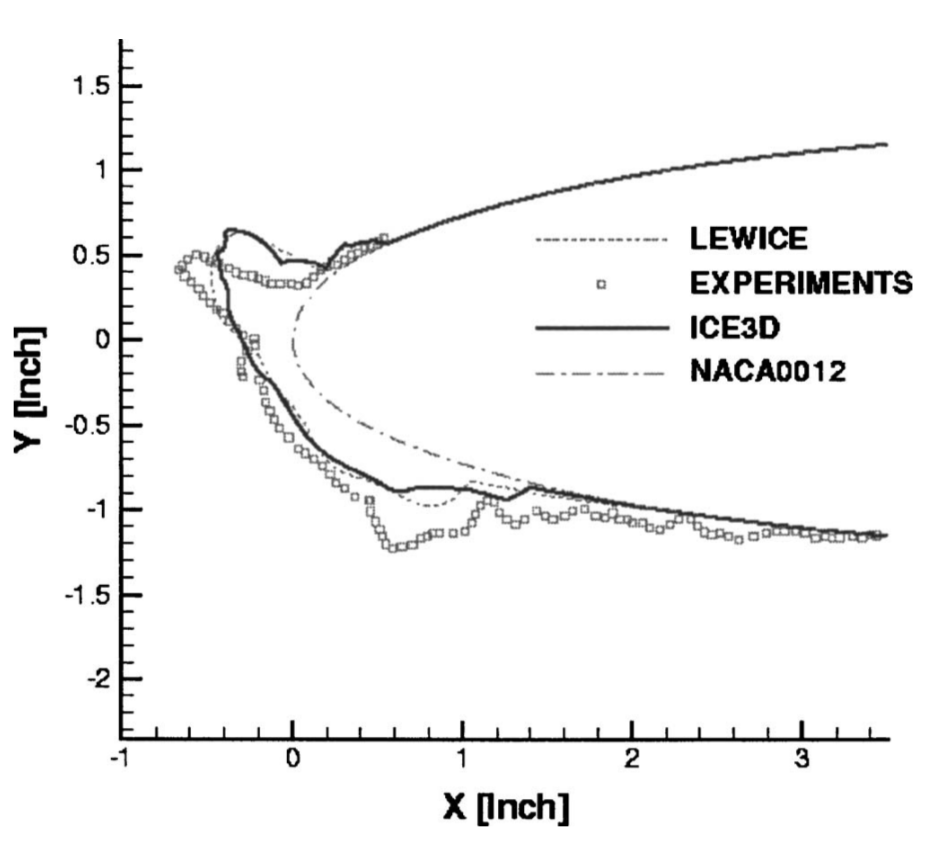
\includegraphics[width=0.4\textwidth]{Habashi2006ShapeVariation}}
      \subfigure[Wright, 2004]{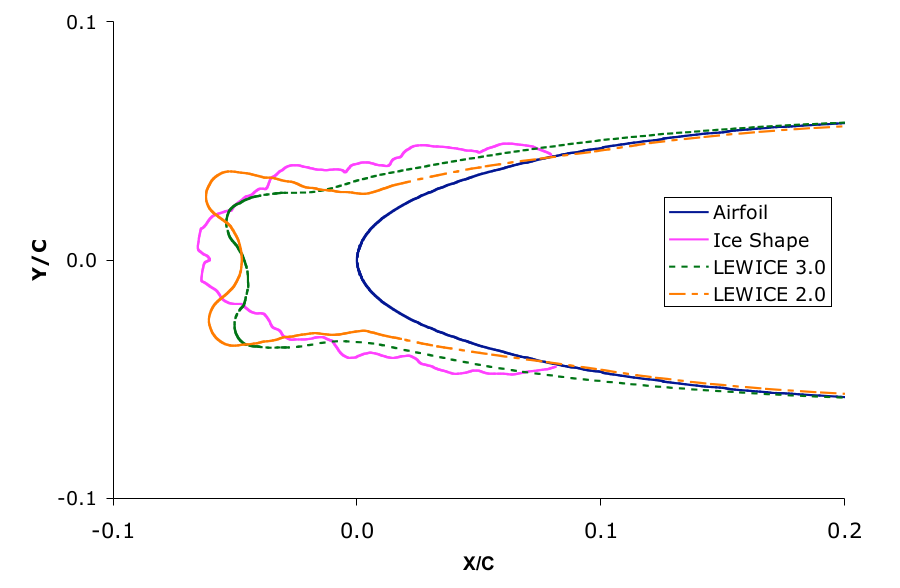
\includegraphics[width=0.4\textwidth]{Wright2004ShapeVariation}}
  \end{subfigmatrix}
\end{figure}

\begin{itemize}
\item Wide variation in experimental/computational ice shapes\footnote{Beaugendre H., Morency M., and Habashi W.G. \emph{Development of a Second Generation in-Flight Icing Simulation Code}. Journal of
Fluids Engineering, ASME, 2006.
 }\textsuperscript{,}\,\footnote{Wright W. and Potapczuk, M.G. \emph{Semi-Empirical Modeling of SLD Physics}, AIAA 2004-412. 42$^{nd}$ AIAA Aerospace Sciences
Meeting, Reno, NV, 2004.
 }
\item Suggests sensitivity to perturbations in underlying physical
  processes
\item \emph{UQ approach:} parameterize the shape variation and study its
  effects on aerodynamics
\end{itemize}
\end{frame}
\section{Icing: UQ Methodology}
\label{sec-2}
\begin{frame}
\frametitle{Input-Process Modeling}
\label{sec-2-1}


\begin{itemize}
\item The space of all ice shapes is infinite dimensional
\item Consider small number of parameters that describe \emph{likely} shapes
\item Analyze database of shapes from experiments/simulations
\item \textbf{Proper Orthogonal Decomposition} \footnote{Holmes P. et. al. \emph{Turbulence, Coherent Structures, Dynamical Systems and Symmetry}, Cambridge University Press, New York, 2012.
 }
\begin{itemize}
\item Assume database of \emph{M} ice shapes
\item Each individual ice shape can be represented by a vector $\bv{x}
    \in \mathbb{R}^N$
\item Approximate $\bv{x}$ using some basis vectors $\psi_i$:
    \begin{equation*}
      \bv{x} \approx \sum_{i=1}^P a_i \psi_i
    \end{equation*}
\item Choose basis vectors to be the eigenvectors of the dataset
    covariance matrix
    \begin{equation*}
    \begin{aligned}
      \mathcal{R} \psi_k = \lambda_k \psi_k& \text{   where:   } \\ 
      \mathcal{R} = \frac{1}{M}\mathbf{X}\mathbf{X}^T \text{   and:   }&
      \mathbf{X} =
       \begin{bmatrix}
        \vline & & \vline \\
        x_1 & \cdots & x_M \\
        \vline & & \vline \\
       \end{bmatrix}
    \end{aligned}
    \end{equation*}
\end{itemize}
\end{itemize}
\end{frame}
\begin{frame}
\frametitle{Polynomial Chaos Expansions (PCE)}
\label{sec-2-2}


\begin{itemize}
\item \textbf{Polynomial Chaos Framework} \footnote{Xiu D. \emph{Numerical Methods for Stochastic Computations: A Spectral Method Approach}. Princeton University Press, 2010.
 }
\begin{itemize}
\item Let $\bv{Z} = (Z_1 \ldots Z_d)$ be $d$ random variables with PDF
    $\rho(\bv{Z})$ that parameterize ice
\item Let $\lbrace \Phi_k \rbrace$ denote the set of polynomials
    which are orthogonal w.r.t. $\rho(\bv{Z})$
\item Let $y(\bv{Z})$ denote the mapping from $\bv{Z}$ to an aerodynamic
    performance metric
\end{itemize}
\item \textbf{Probabilistic Collocation Method:}
\begin{itemize}
\item \emph{Representation} 
    \begin{equation*}
      y(\bv{Z}) \approx \sum_{|i|=0}^N y_i \Phi_i(\bv{Z})
    \end{equation*}
\item \emph{Orthonormality} 
    \begin{equation*}
    \begin{aligned}
      \ip{f}{g} &= \int_{\Gamma} f(\bv{z})g(\bv{z}) \rho(\bv{z}) d\bv{z} \\
      \ip{\Phi_i}{\Phi_j} &= \delta_{ij}
    \end{aligned}
    \end{equation*}
\item \emph{Quadrature} 
    \begin{equation*}
      y_k = \ip{y}{\Phi_k} \approx \sum_{i=0}^{Q}
    y(\bv{Z}^{(k)}) \Phi_k(\bv{Z}^{(k)}) w_k
    \end{equation*}
\end{itemize}
\end{itemize}
\end{frame}
\begin{frame}
\frametitle{PCE with Sparse Grids}
\label{sec-2-3}


\begin{columns}[c]
  \column{0.7\textwidth}
    \centering
    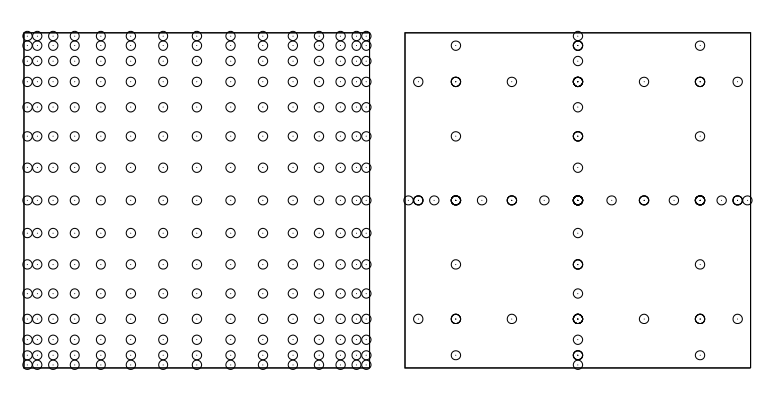
\includegraphics[width=0.95\textwidth]{SparseGrid1} \\
    \bf{Full Tensor Product vs. Sparse Grid}
  \column{0.3\textwidth}
    \centering
    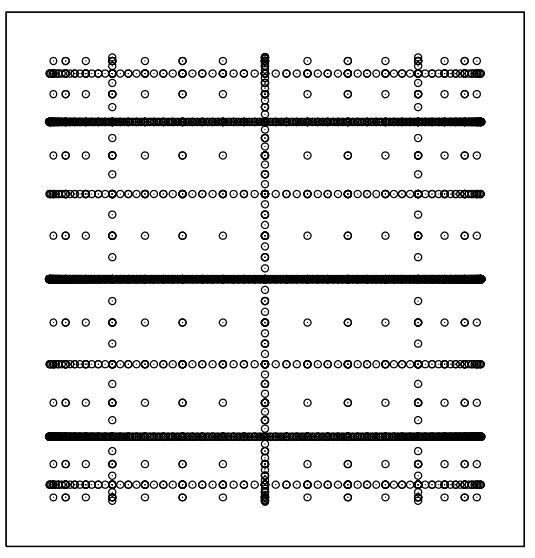
\includegraphics[width=0.95\textwidth]{SparseGrid2} \\
    {\bf Anisotropic Grid}
\end{columns}

\begin{itemize}
\item \textbf{Sparse Grids}\footnote{LeMaitre O. \emph{Spectral Methods for Uncertainty Quantification}. Springer, 2010.
 }
\begin{itemize}
\item \emph{Efficient}: Only a subset of the full quadrature grid is used
\begin{itemize}
\item For $d >> 1$, number of samples scales as $2^N {N+d \choose d} <<
      (N+1)^d$
\end{itemize}
\item \emph{Adaptive}: Start with a coarse mesh, adaptively refine until
    achieve desired resolution
\item \emph{Anisotropic}: Refine grid in most ``important'' directions
\item Implemented in DAKOTA\footnote{Adams et. al. \emph{DAKOTA, A Multilevel Parallel Object-Oriented Framework for Design Optimization\ldots{}} V. 5.3 User's
Manual. SAND2010-2183.
 } (open-source UQ code)
\end{itemize}
\end{itemize}
\end{frame}
\section{Icing: Data-Based UQ}
\label{sec-3}
\begin{frame}
\frametitle{Heuristic Input Processes}
\label{sec-3-1}


\begin{columns}[c]
  \column{0.33\textwidth}
    \centering
    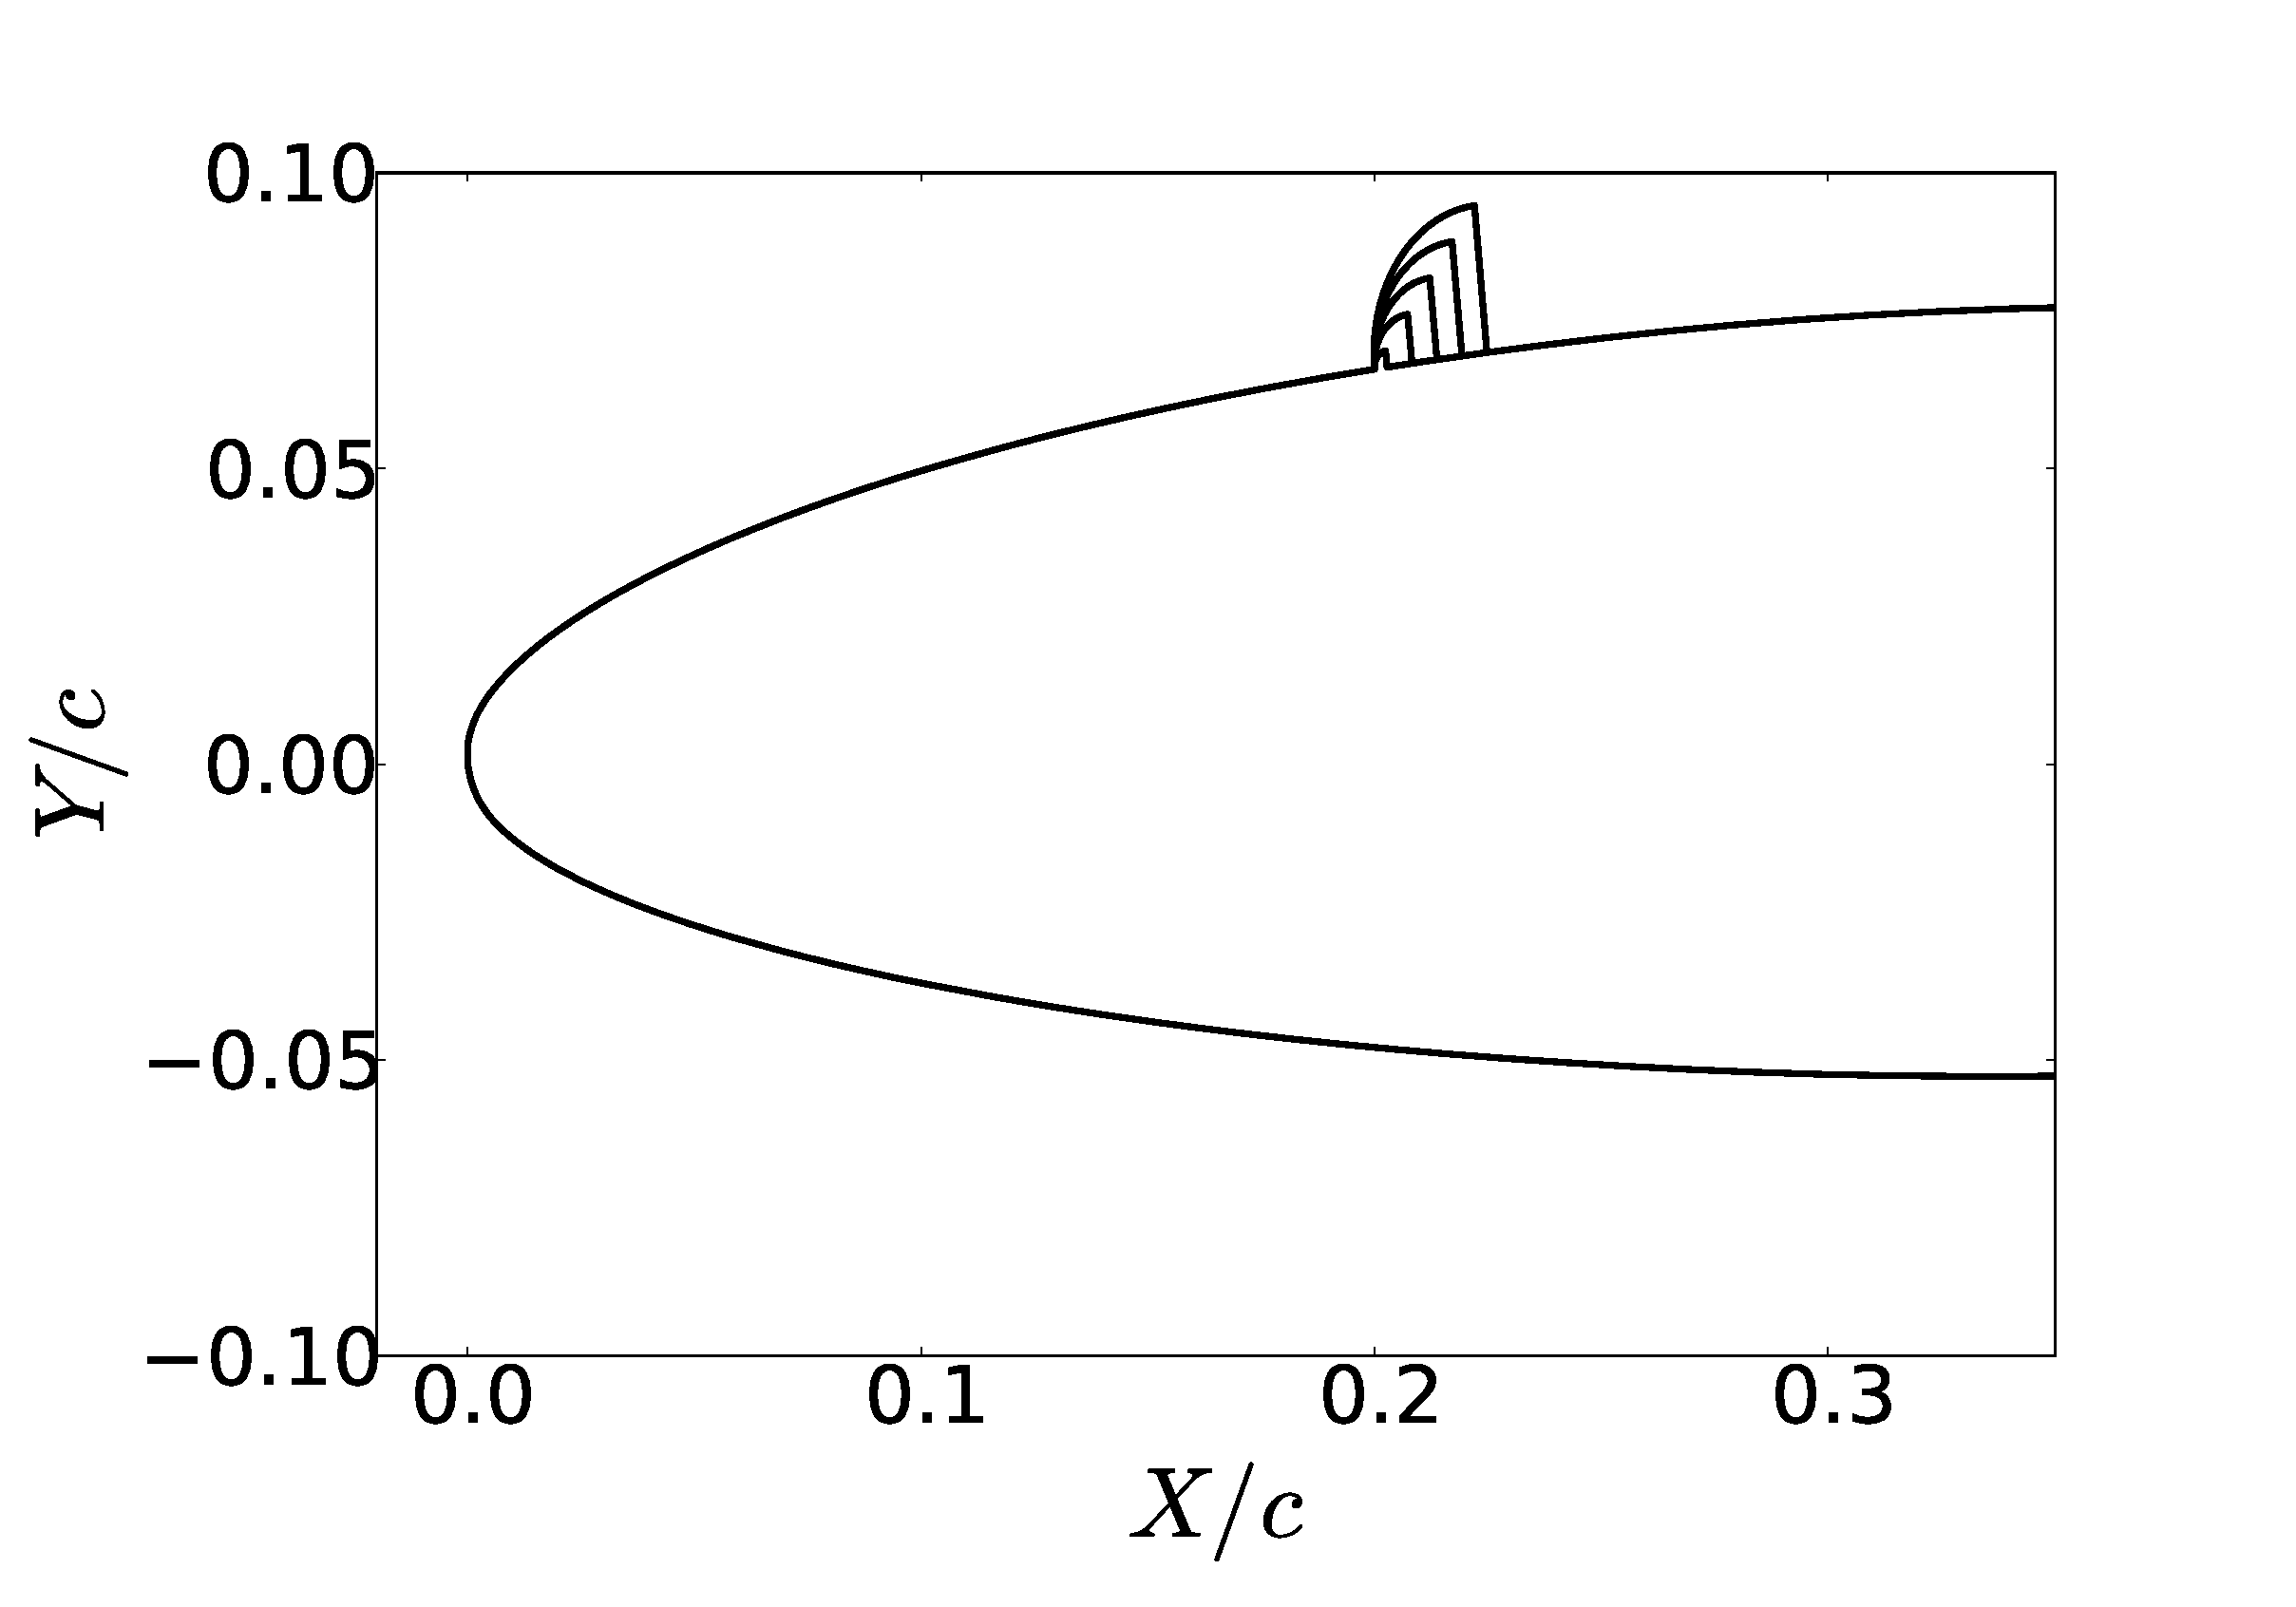
\includegraphics[width=0.95\textwidth]{RidgeRVariation} \\
    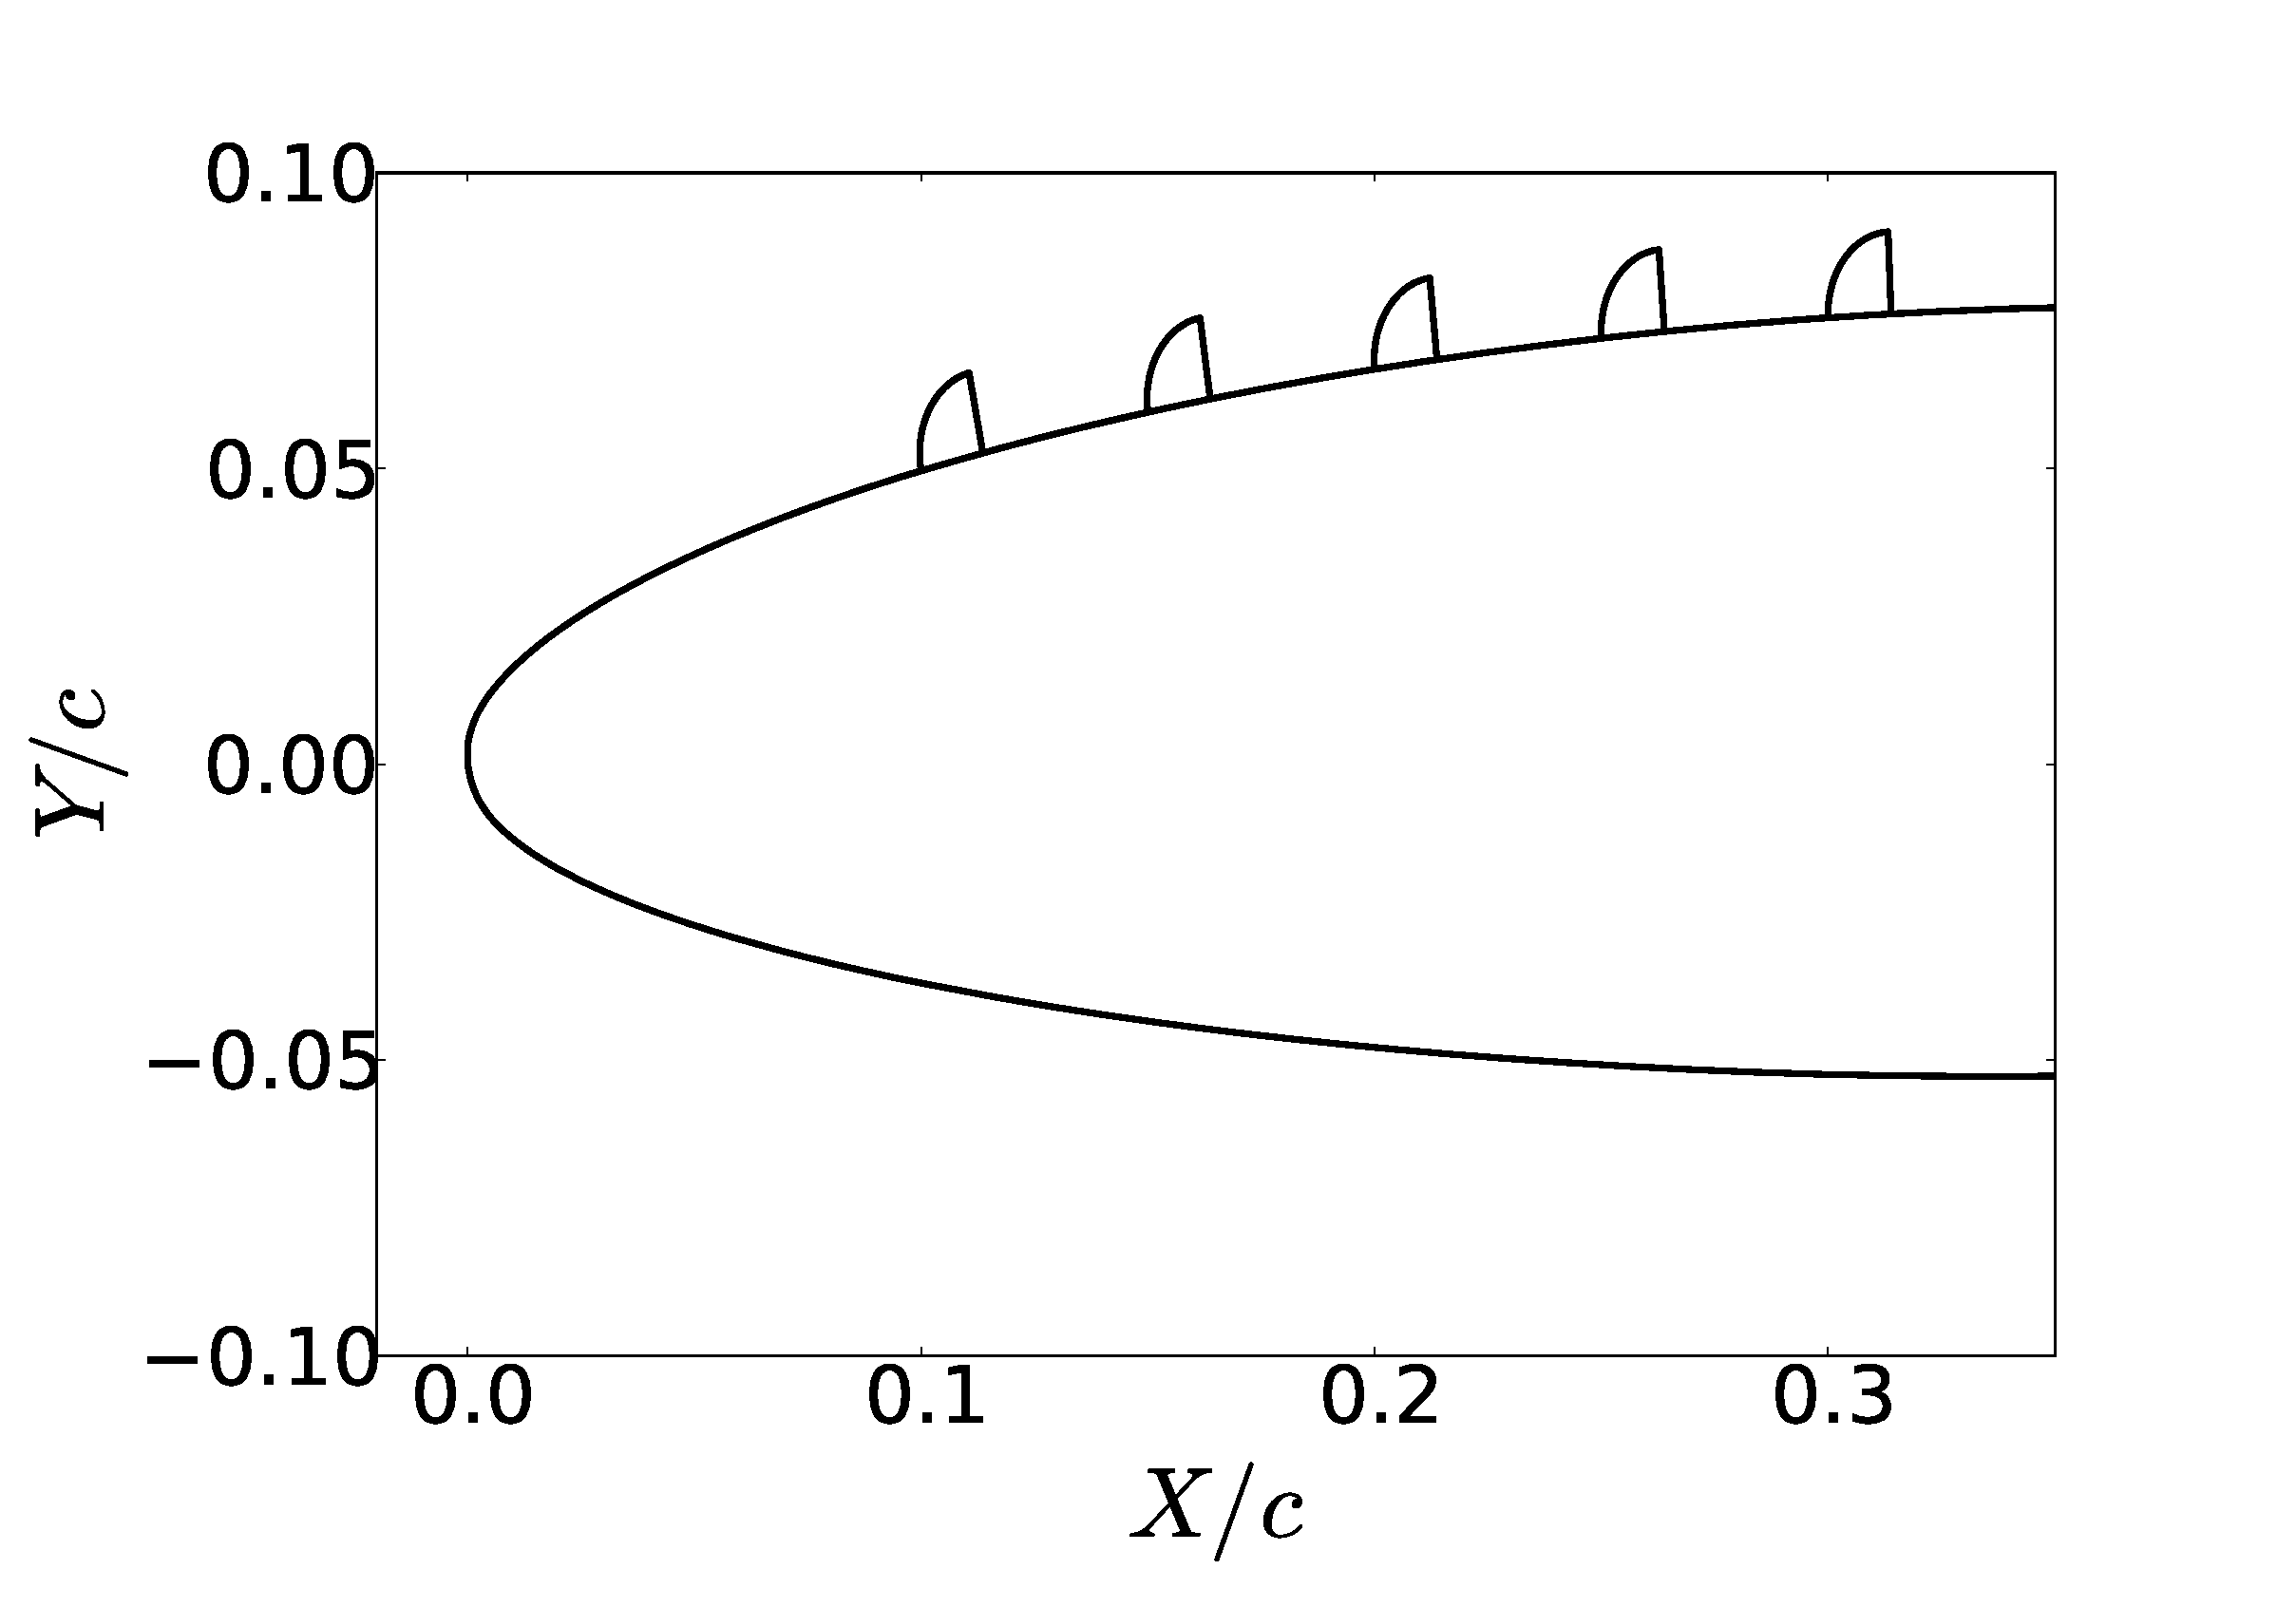
\includegraphics[width=0.95\textwidth]{RidgeSVariation} \\
    {\bf Ridge}
  \column{0.33\textwidth}
    \centering
    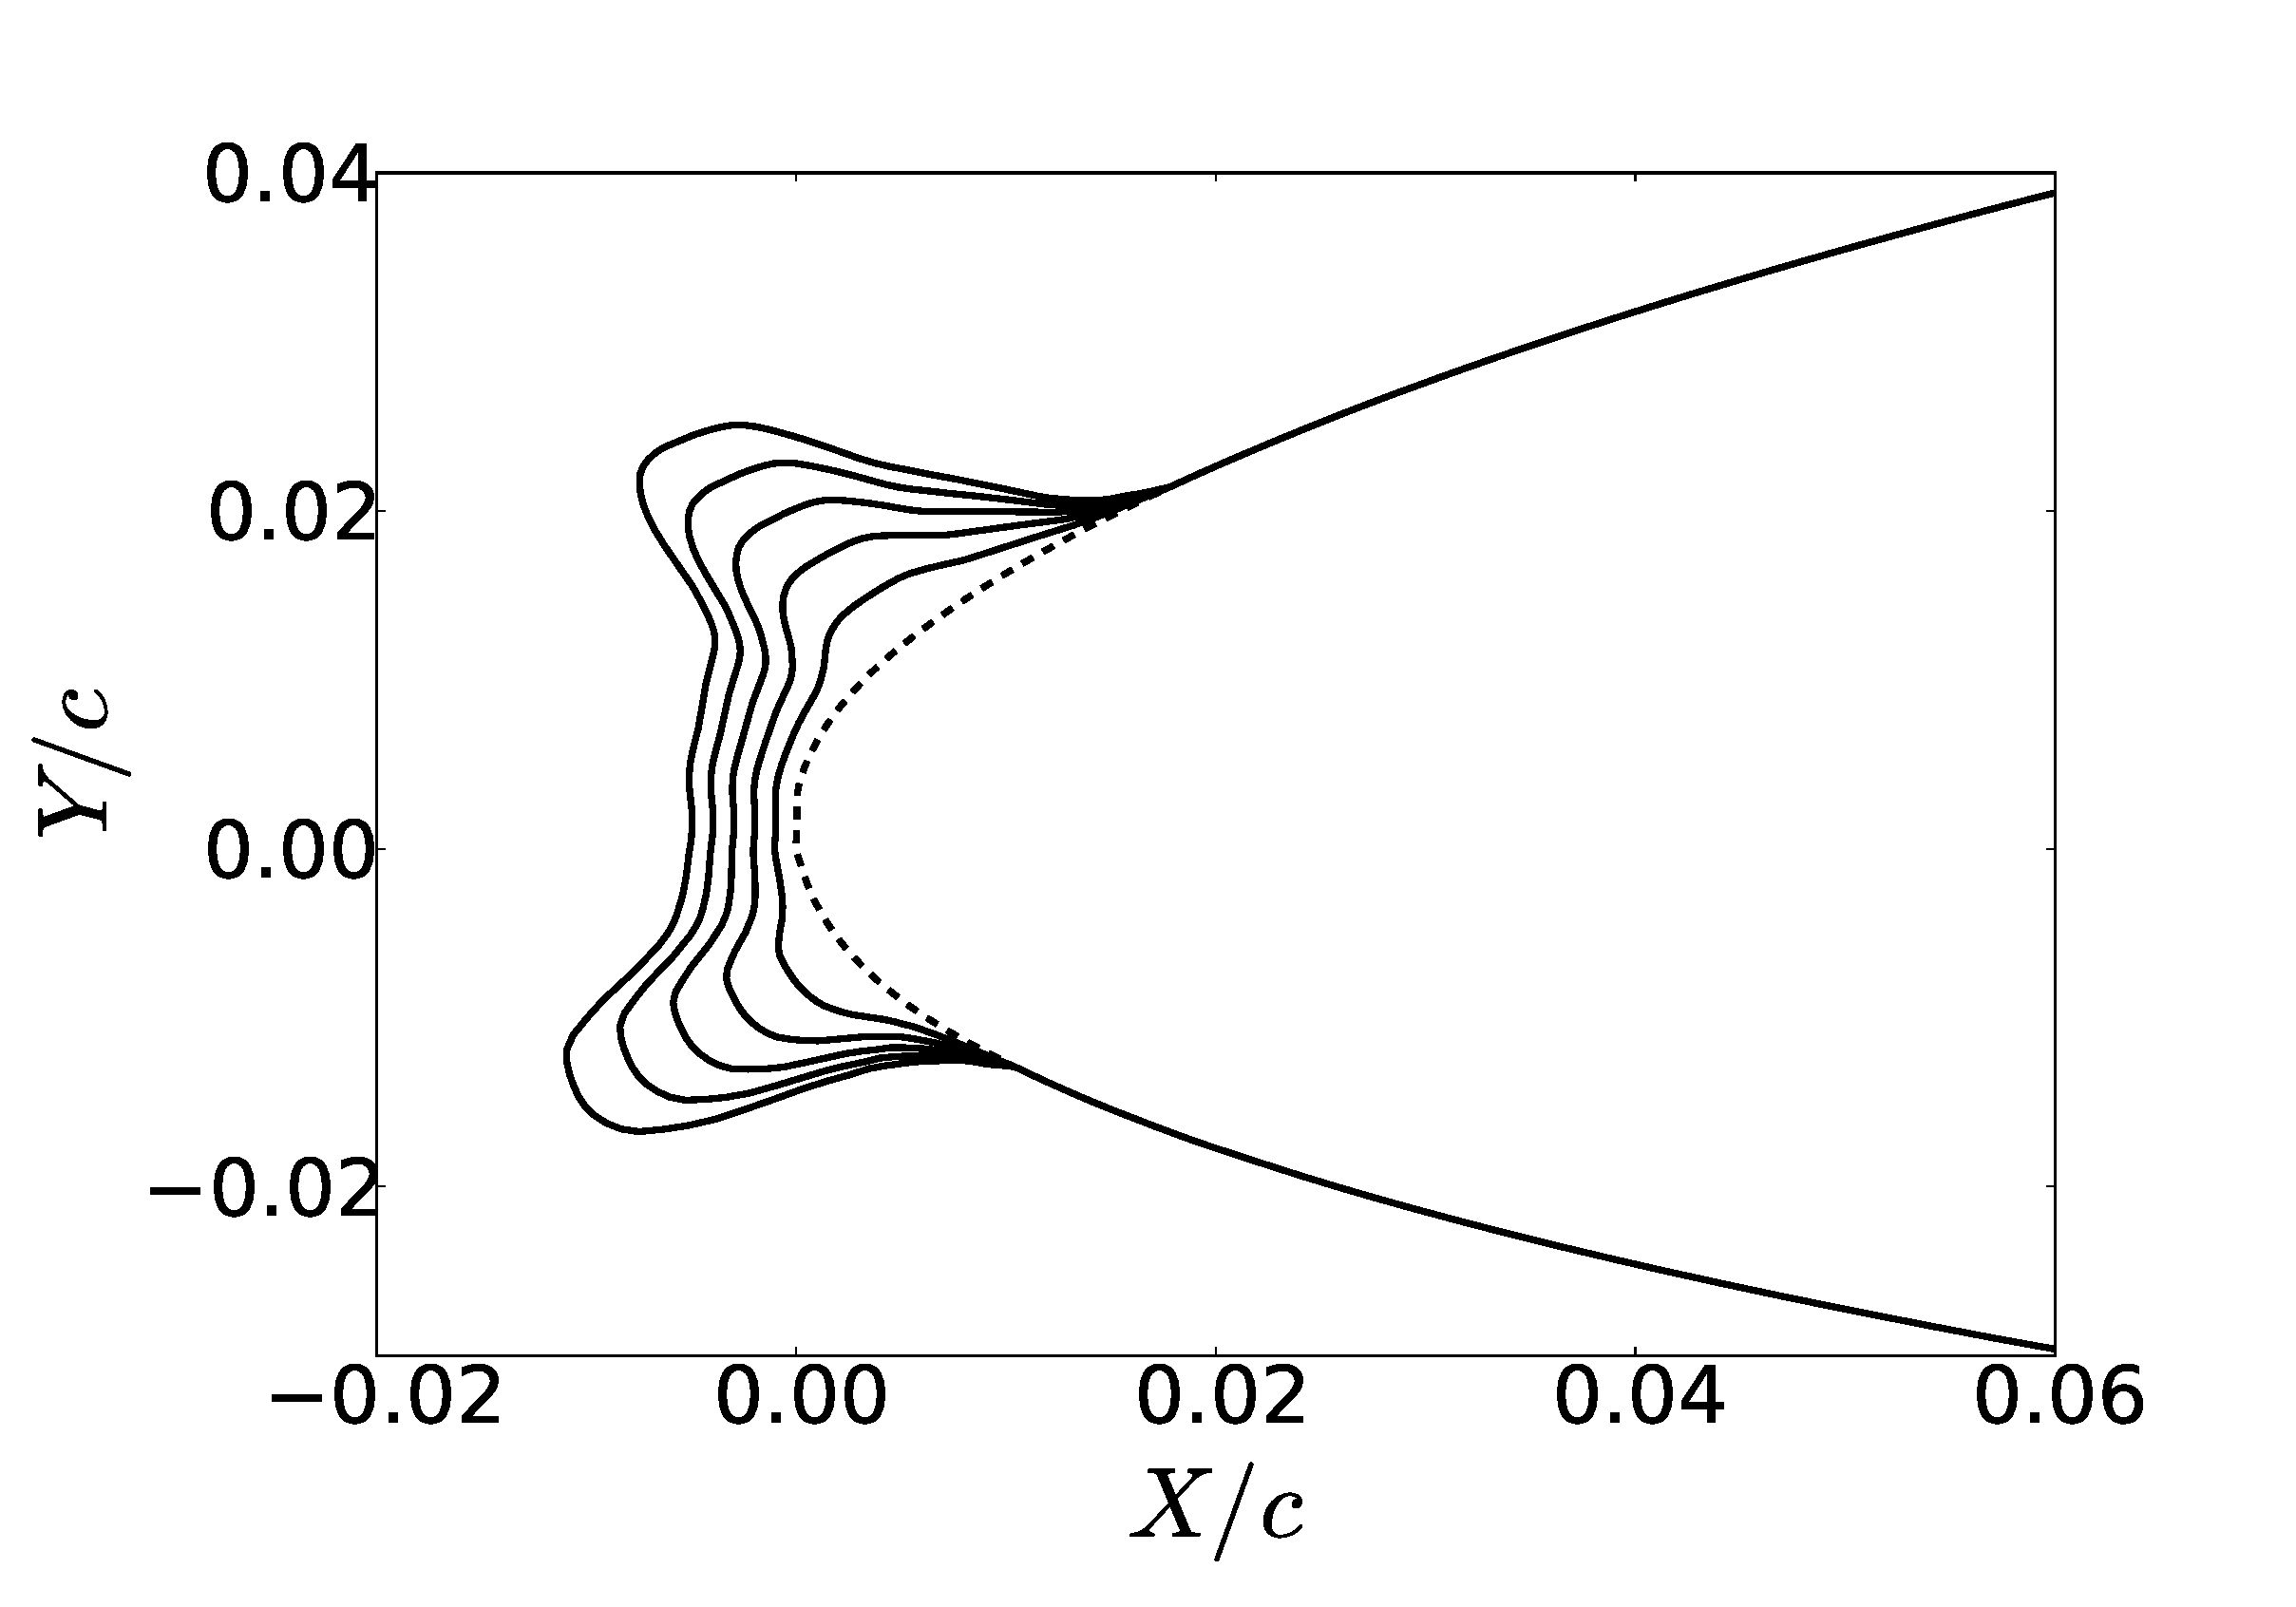
\includegraphics[width=0.95\textwidth]{HornHVariation} \\
    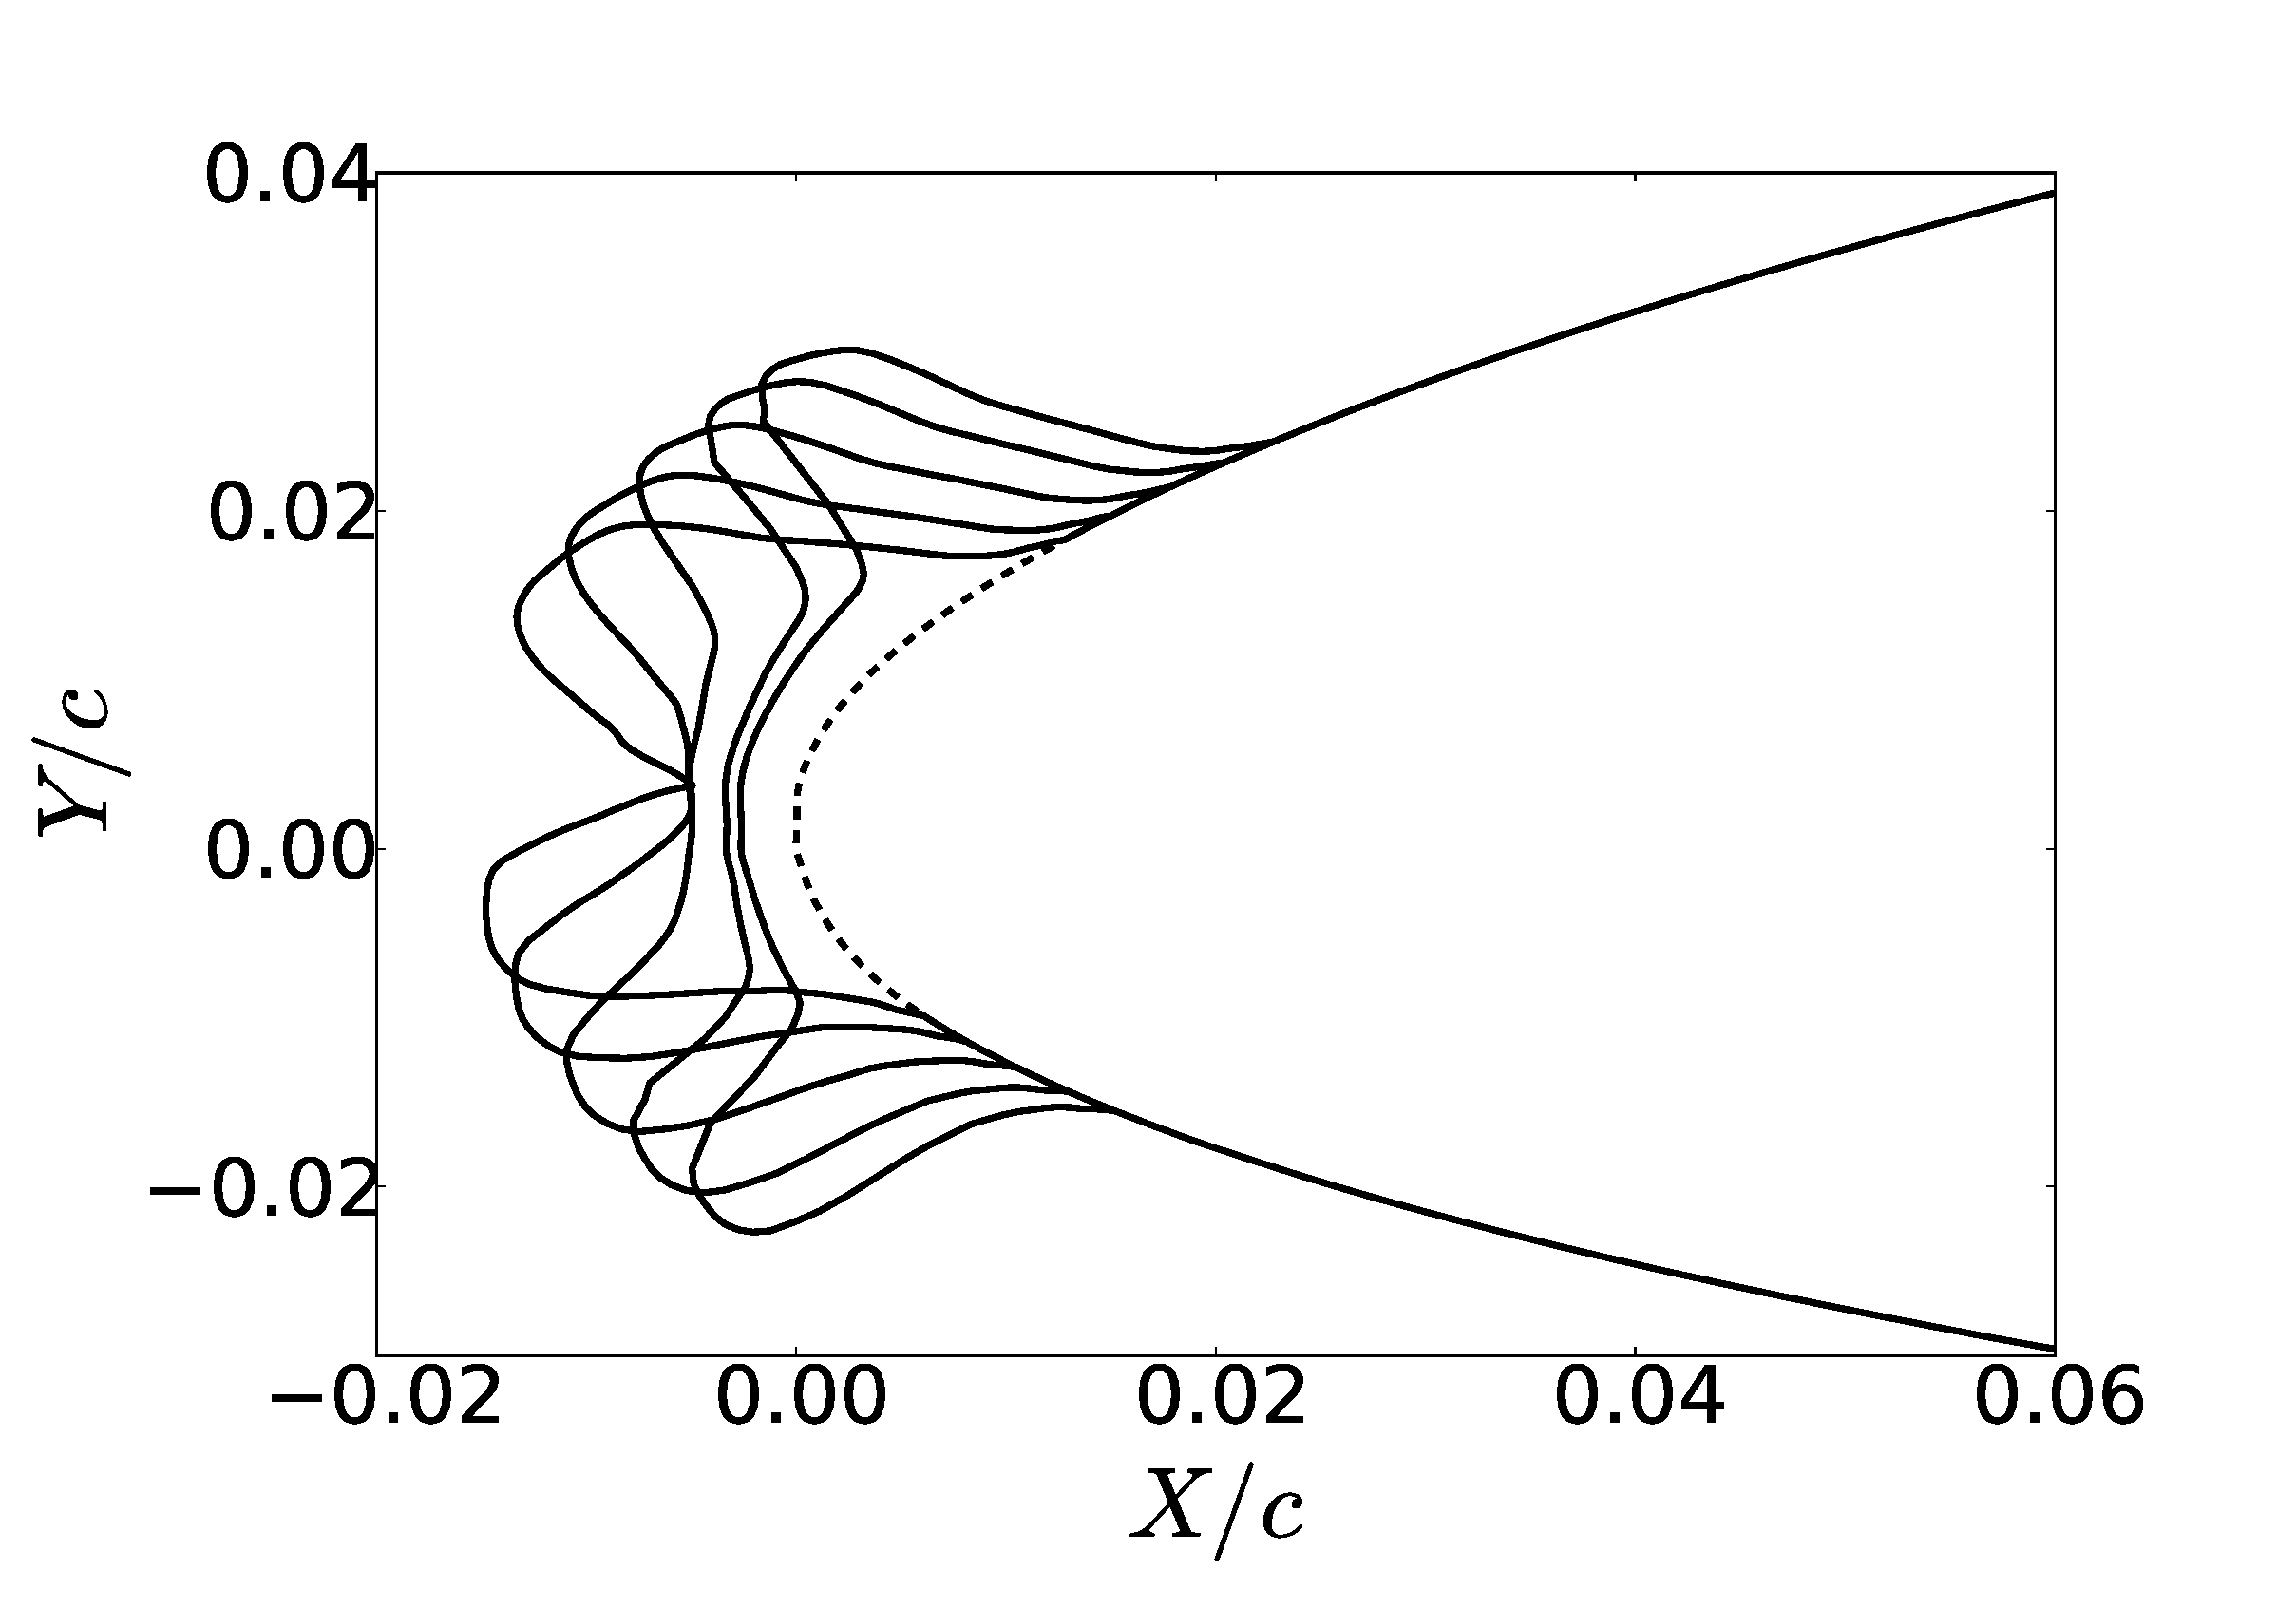
\includegraphics[width=0.95\textwidth]{HornSVariation} \\
    {\bf Horn}
  \column{0.33\textwidth}
    \centering    
    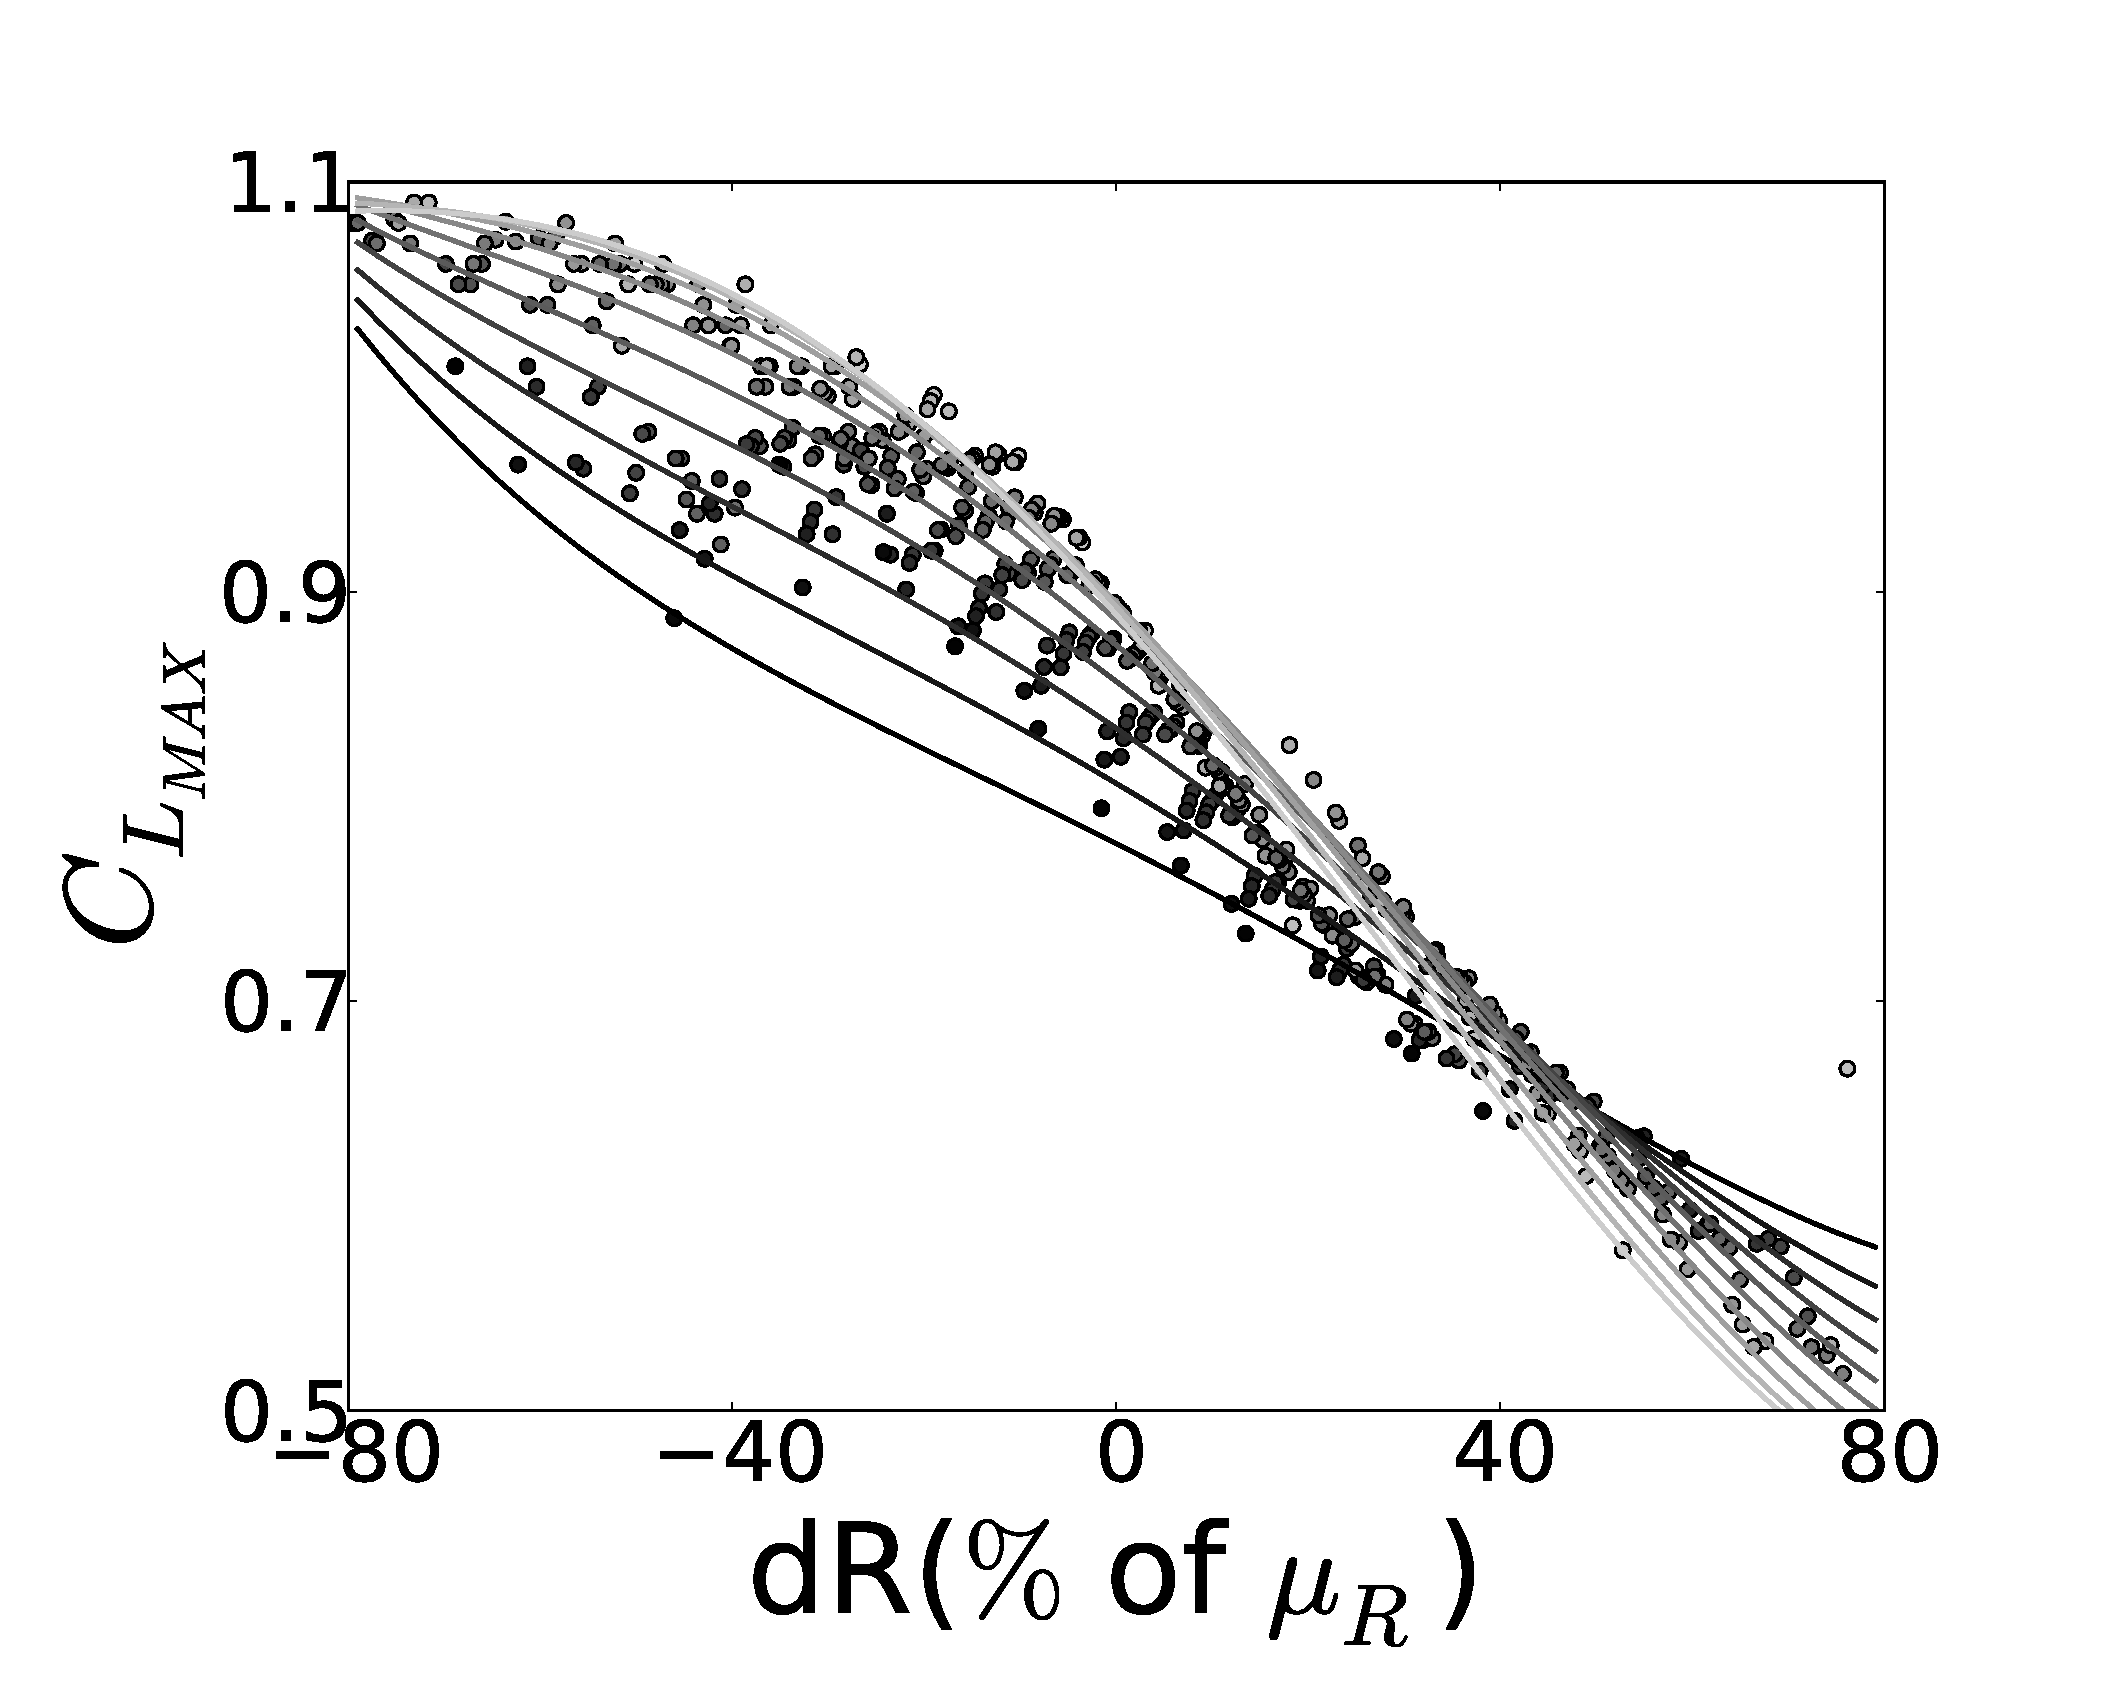
\includegraphics[width=0.9\textwidth]{MC_surrogate_LargeUnc_CL} \\
    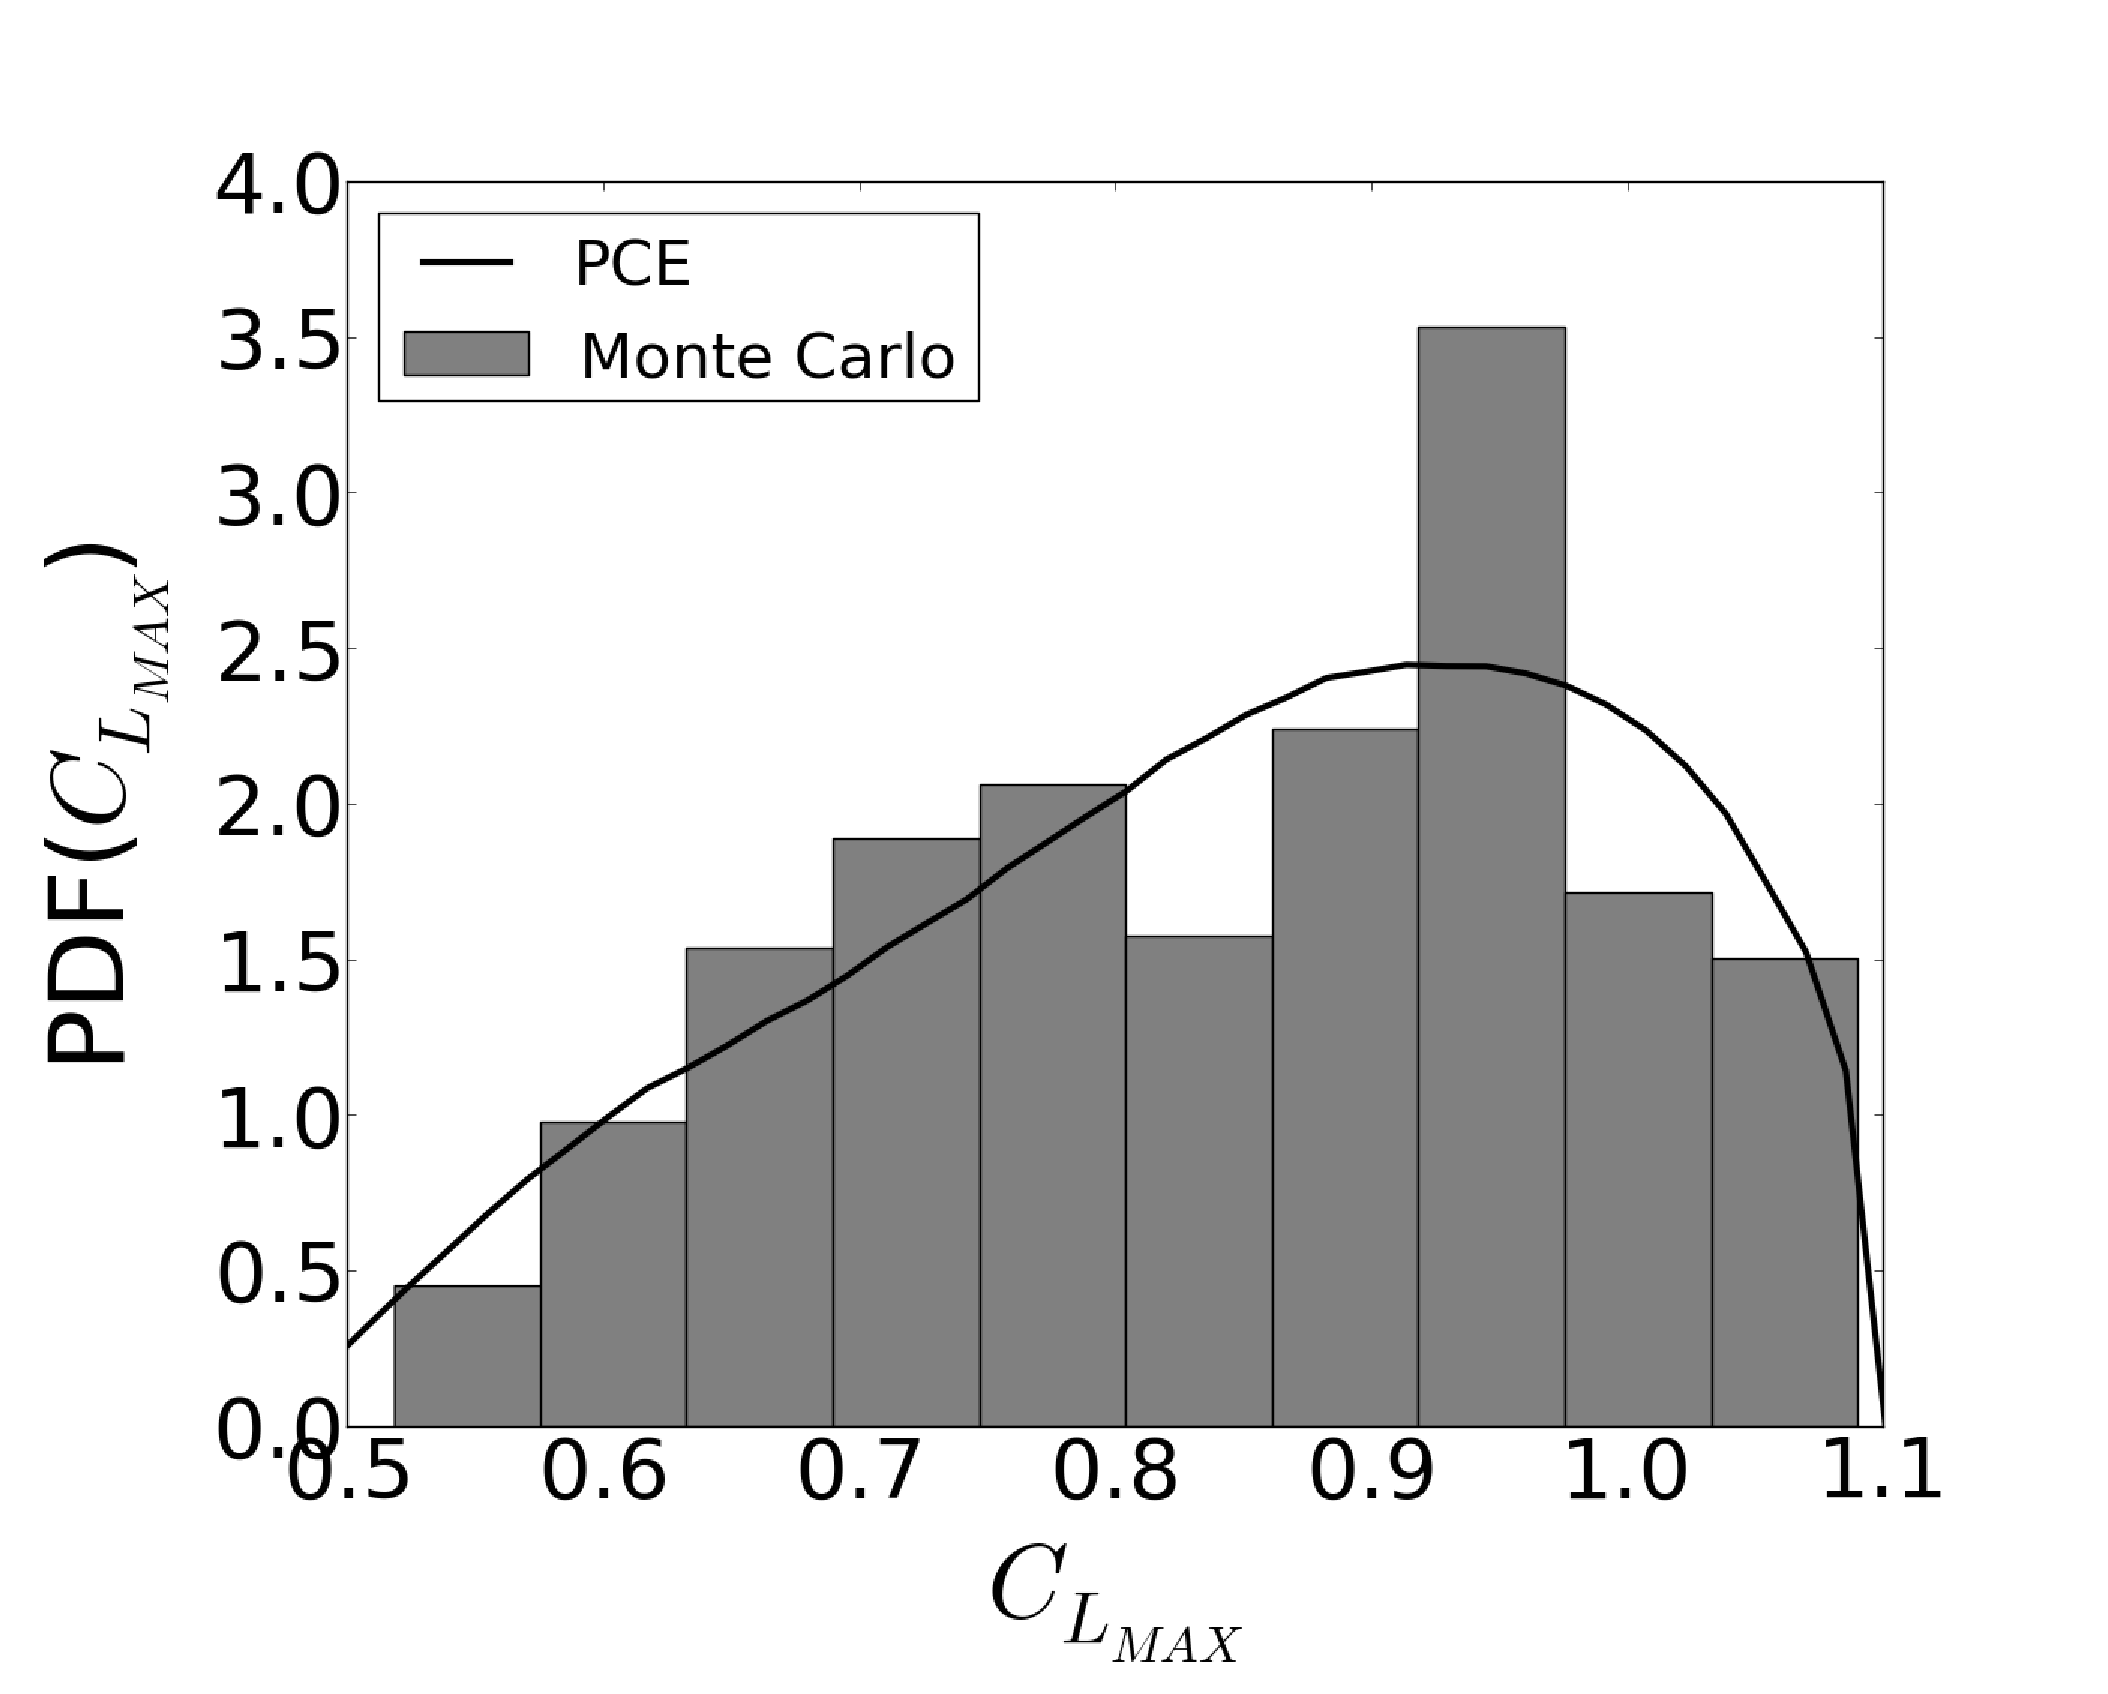
\includegraphics[width=0.9\textwidth]{MCgpcPDFLargeUnc_CL} \\
    {\bf Statistics}
\end{columns}

\begin{itemize}
\item Previous study examined parameterized ridge and horn ice
  shapes\footnote{DeGennaro A., Rowley C.W., and Martinelli,
L. \emph{Uncertainty Quantification for Airfoil Icing using Polynomial Chaos Expansions}. To appear in Journal of Aircraft, 2015.
 }
\item Approach was heuristic, not directly based on observed shape
  variations
\item Parameter space was low dimensional; no low-dimensional modeling
\end{itemize}
\end{frame}
\begin{frame}
\frametitle{Data-Based Input Processes: 3D Wing}
\label{sec-3-2}

\begin{figure}
  \centering
  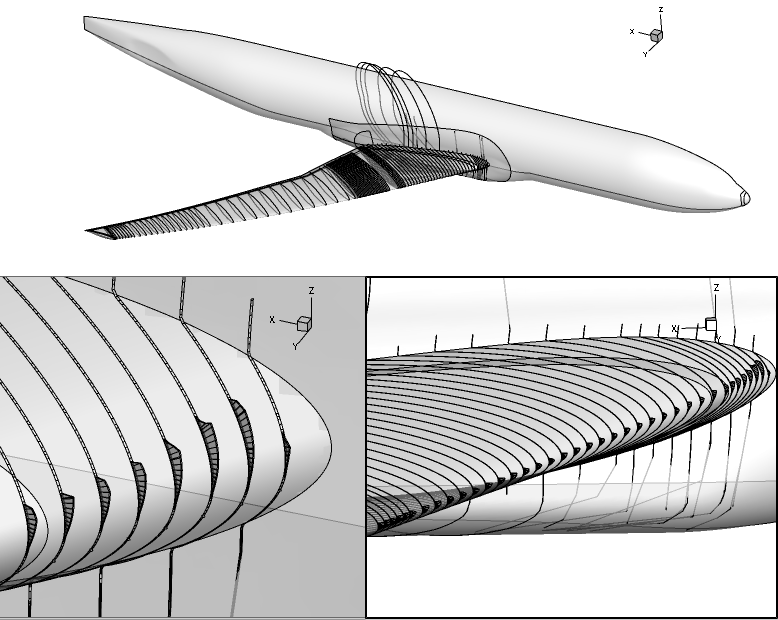
\includegraphics[width=0.6\textwidth]{CRMHorn}
\end{figure}

\begin{itemize}
\item NASA Common Research Model (CRM), $65\%$ scale\footnote{Broeren A. et. al. \emph{Swept-Wing Ice Accretion Characterization and Aerodynamics}, AIAA 2013-2824.
 }
\begin{itemize}
\item 45 min accretion time, altitude = 10,000 ft, velocity = 232 knots,
    temperature = $-4^{\text{o}}$ C, MVD = 20 $\mu m$, LWC = 0.55
    $g/m^3$
\end{itemize}
\end{itemize}
\end{frame}
\begin{frame}
\frametitle{Data-Based Input Processes: 3D Wing}
\label{sec-3-3}

\begin{columns}[c]
  \column{0.3\textwidth}
    \centering
    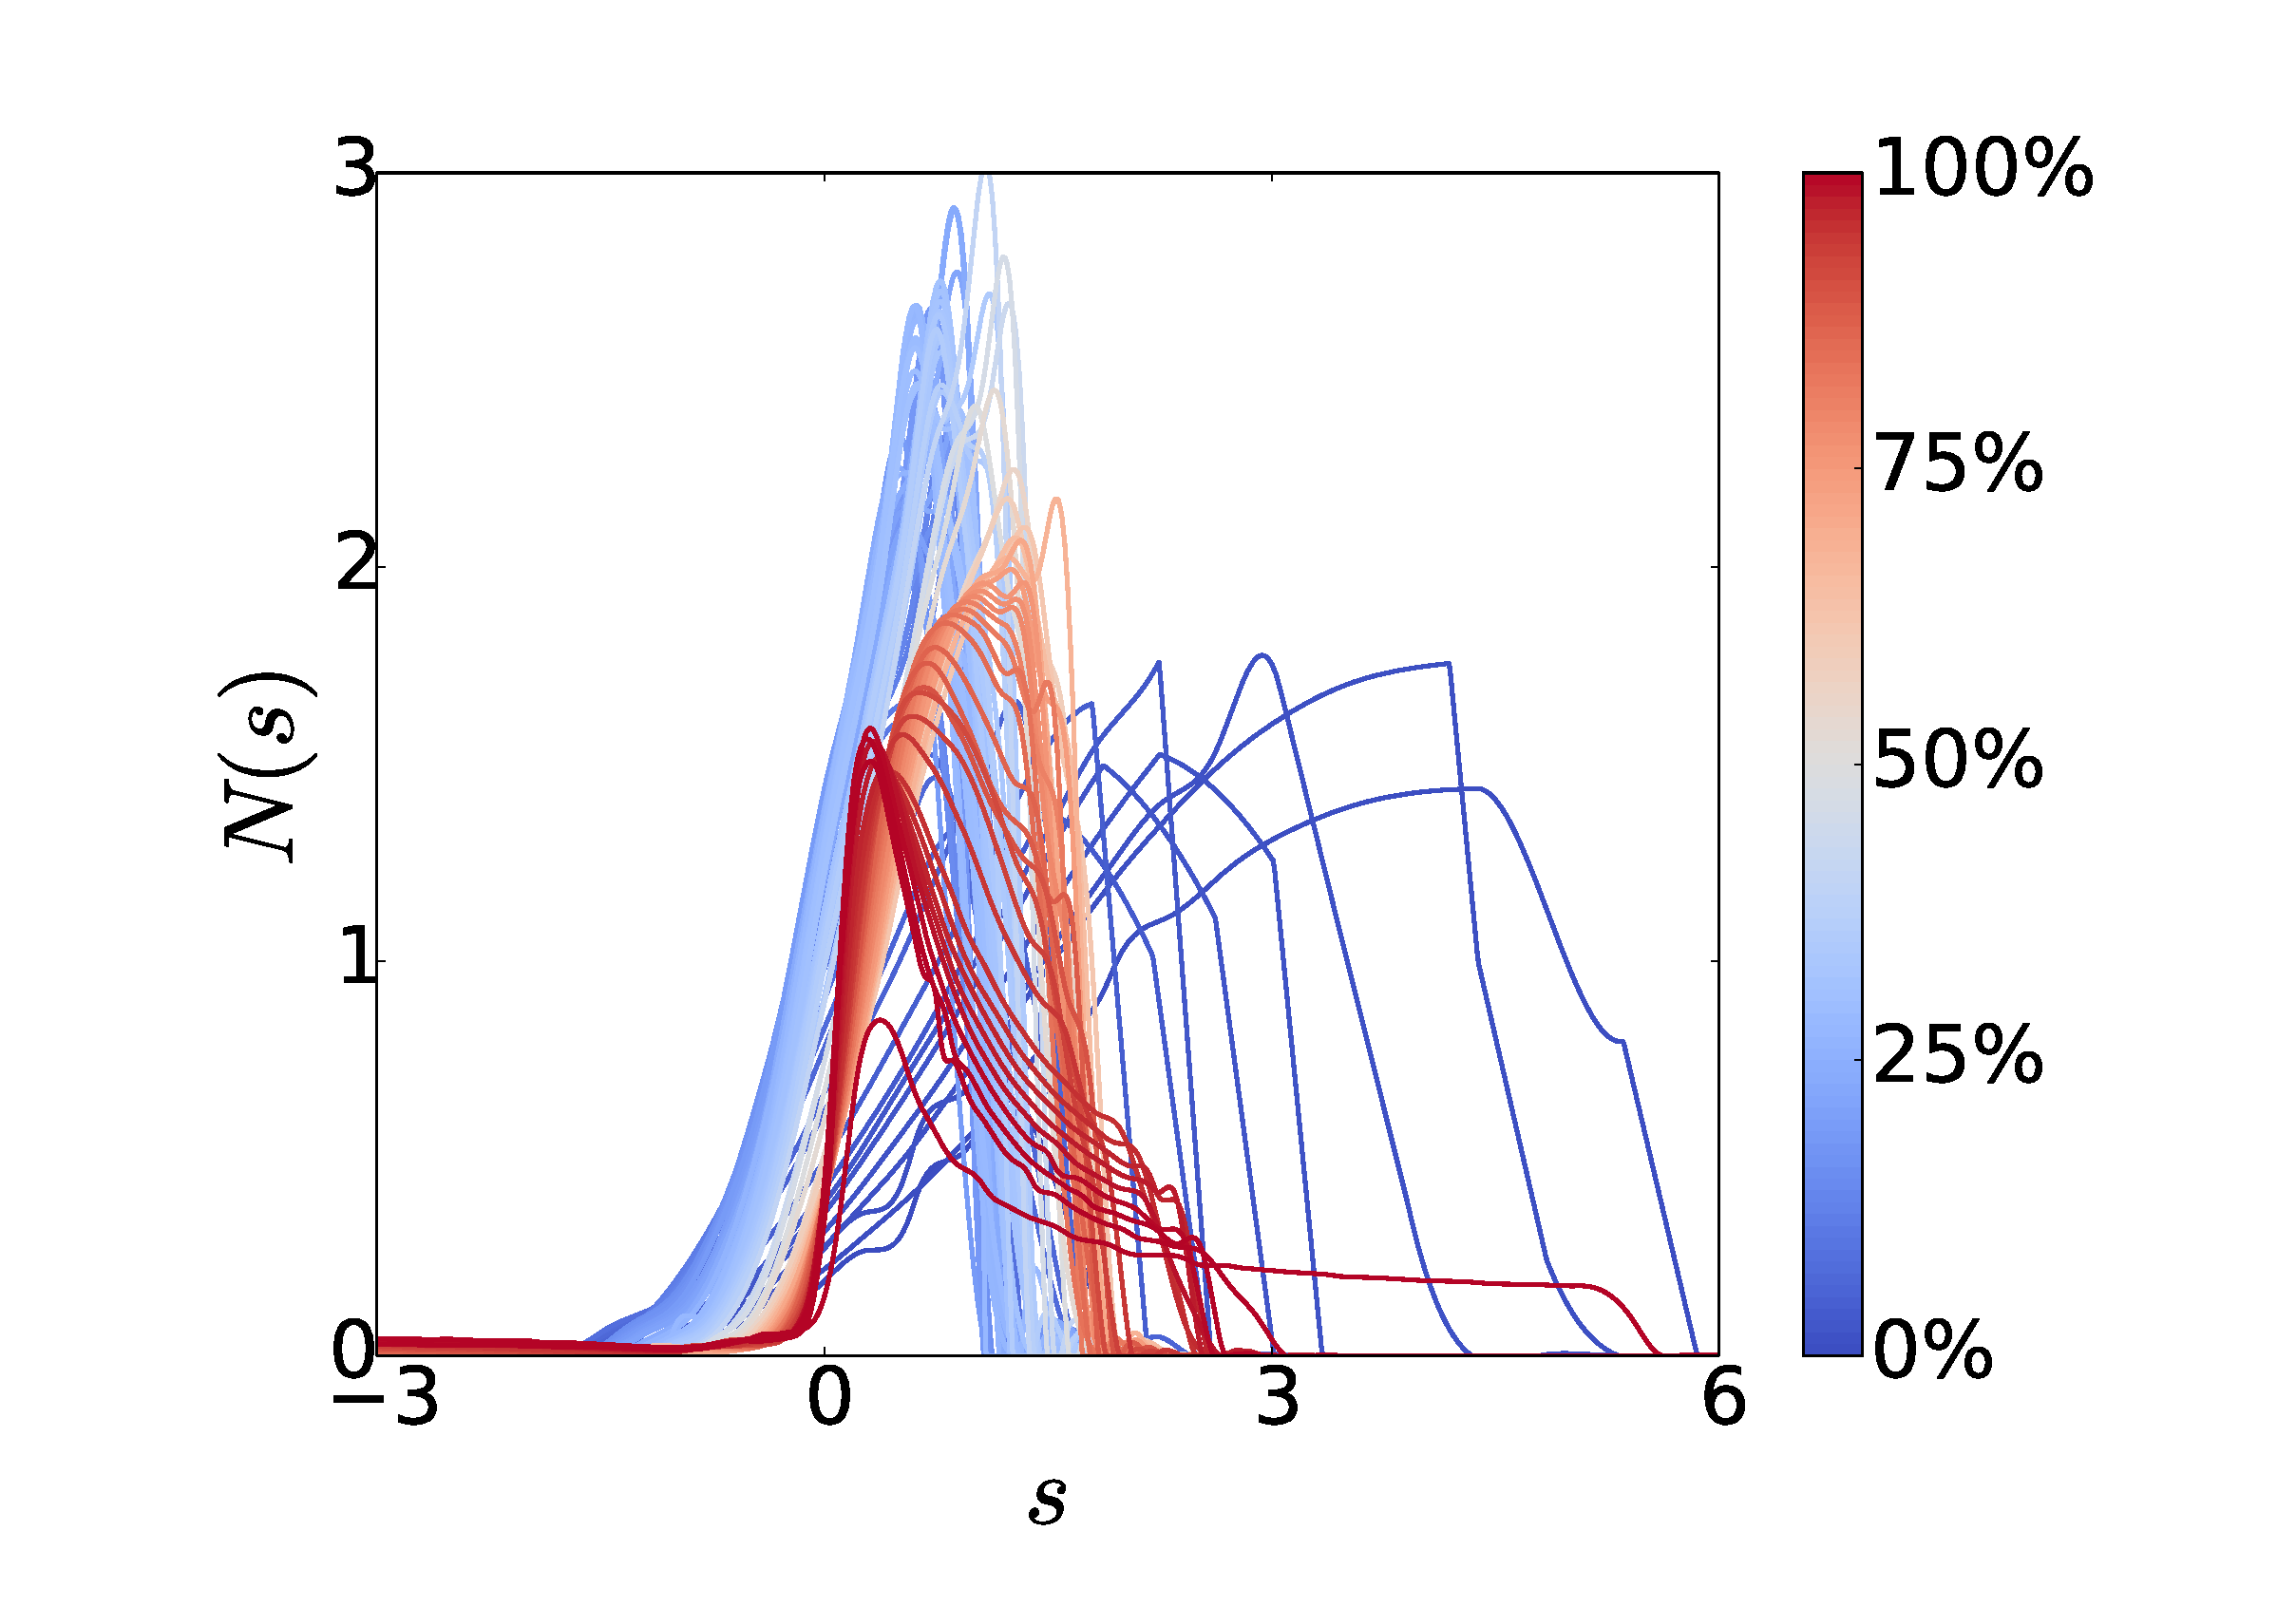
\includegraphics[width=1.3\textwidth]{HornsUnaligned} \\
    \bf{Original Data}
  \column{0.3\textwidth}
    \centering
    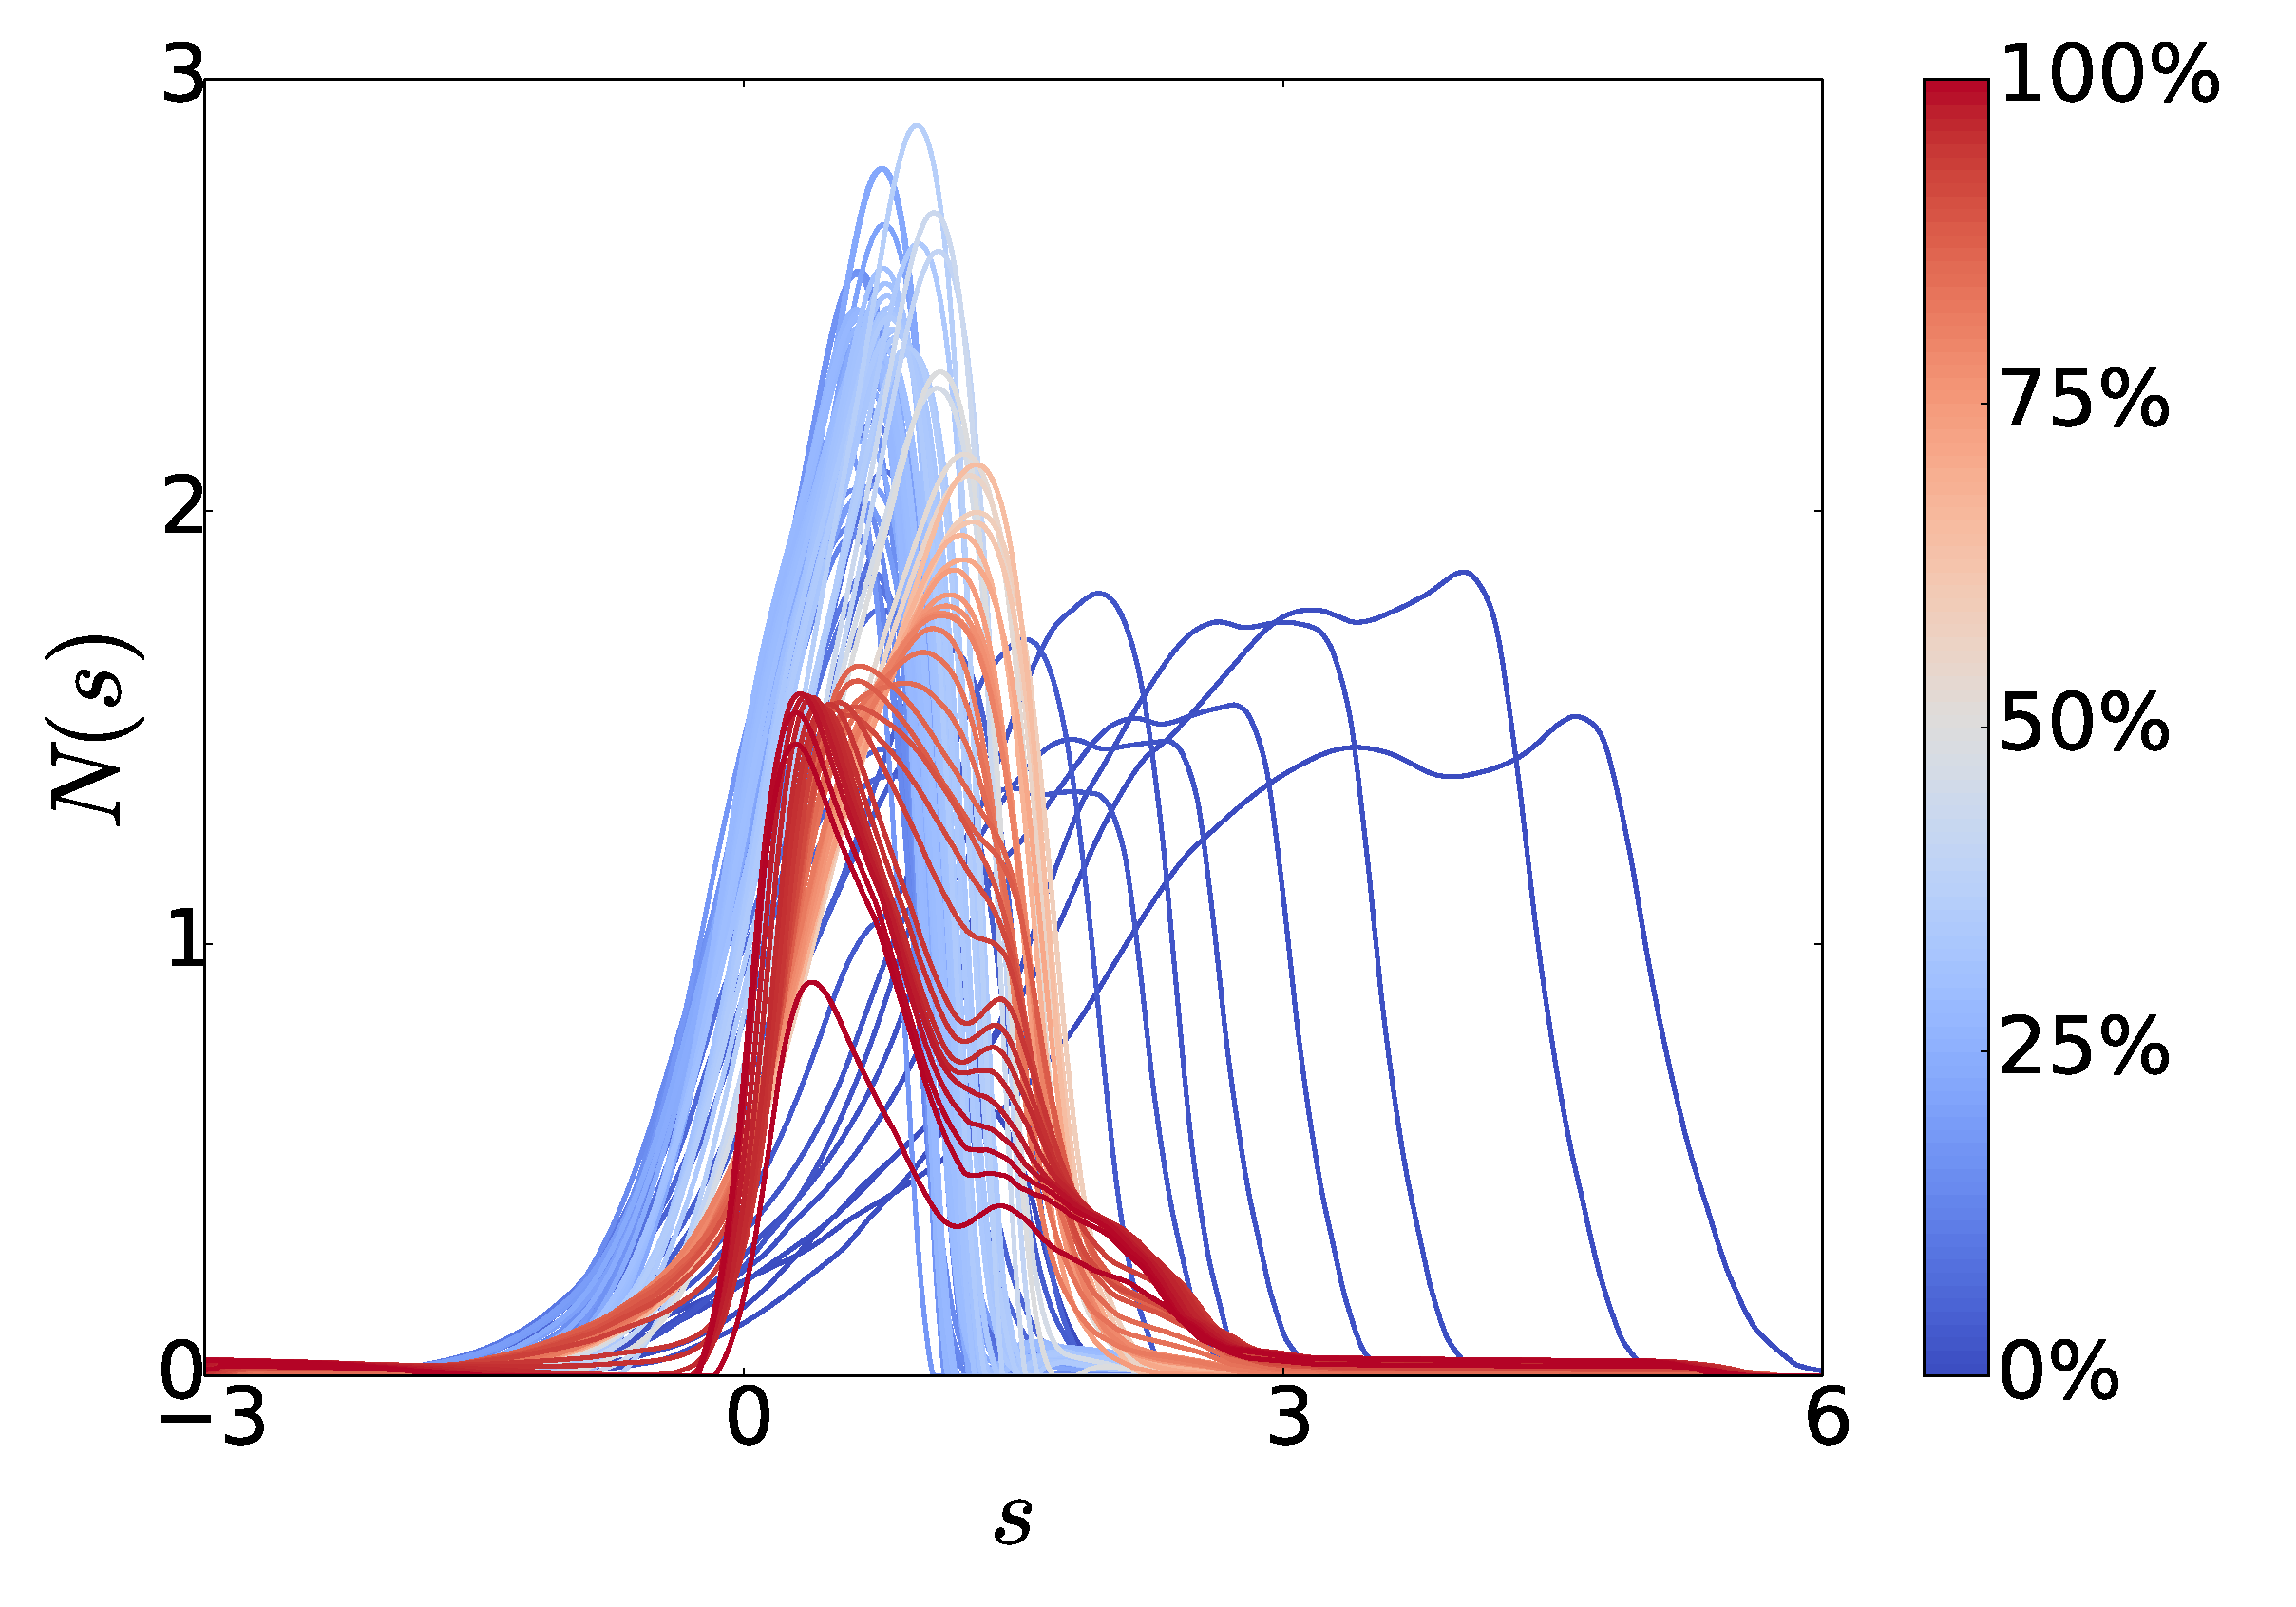
\includegraphics[width=1.25\textwidth]{PODReconstruction2} \\
    {\bf POD Reconstruction}
  \column{0.3\textwidth}
    \centering
    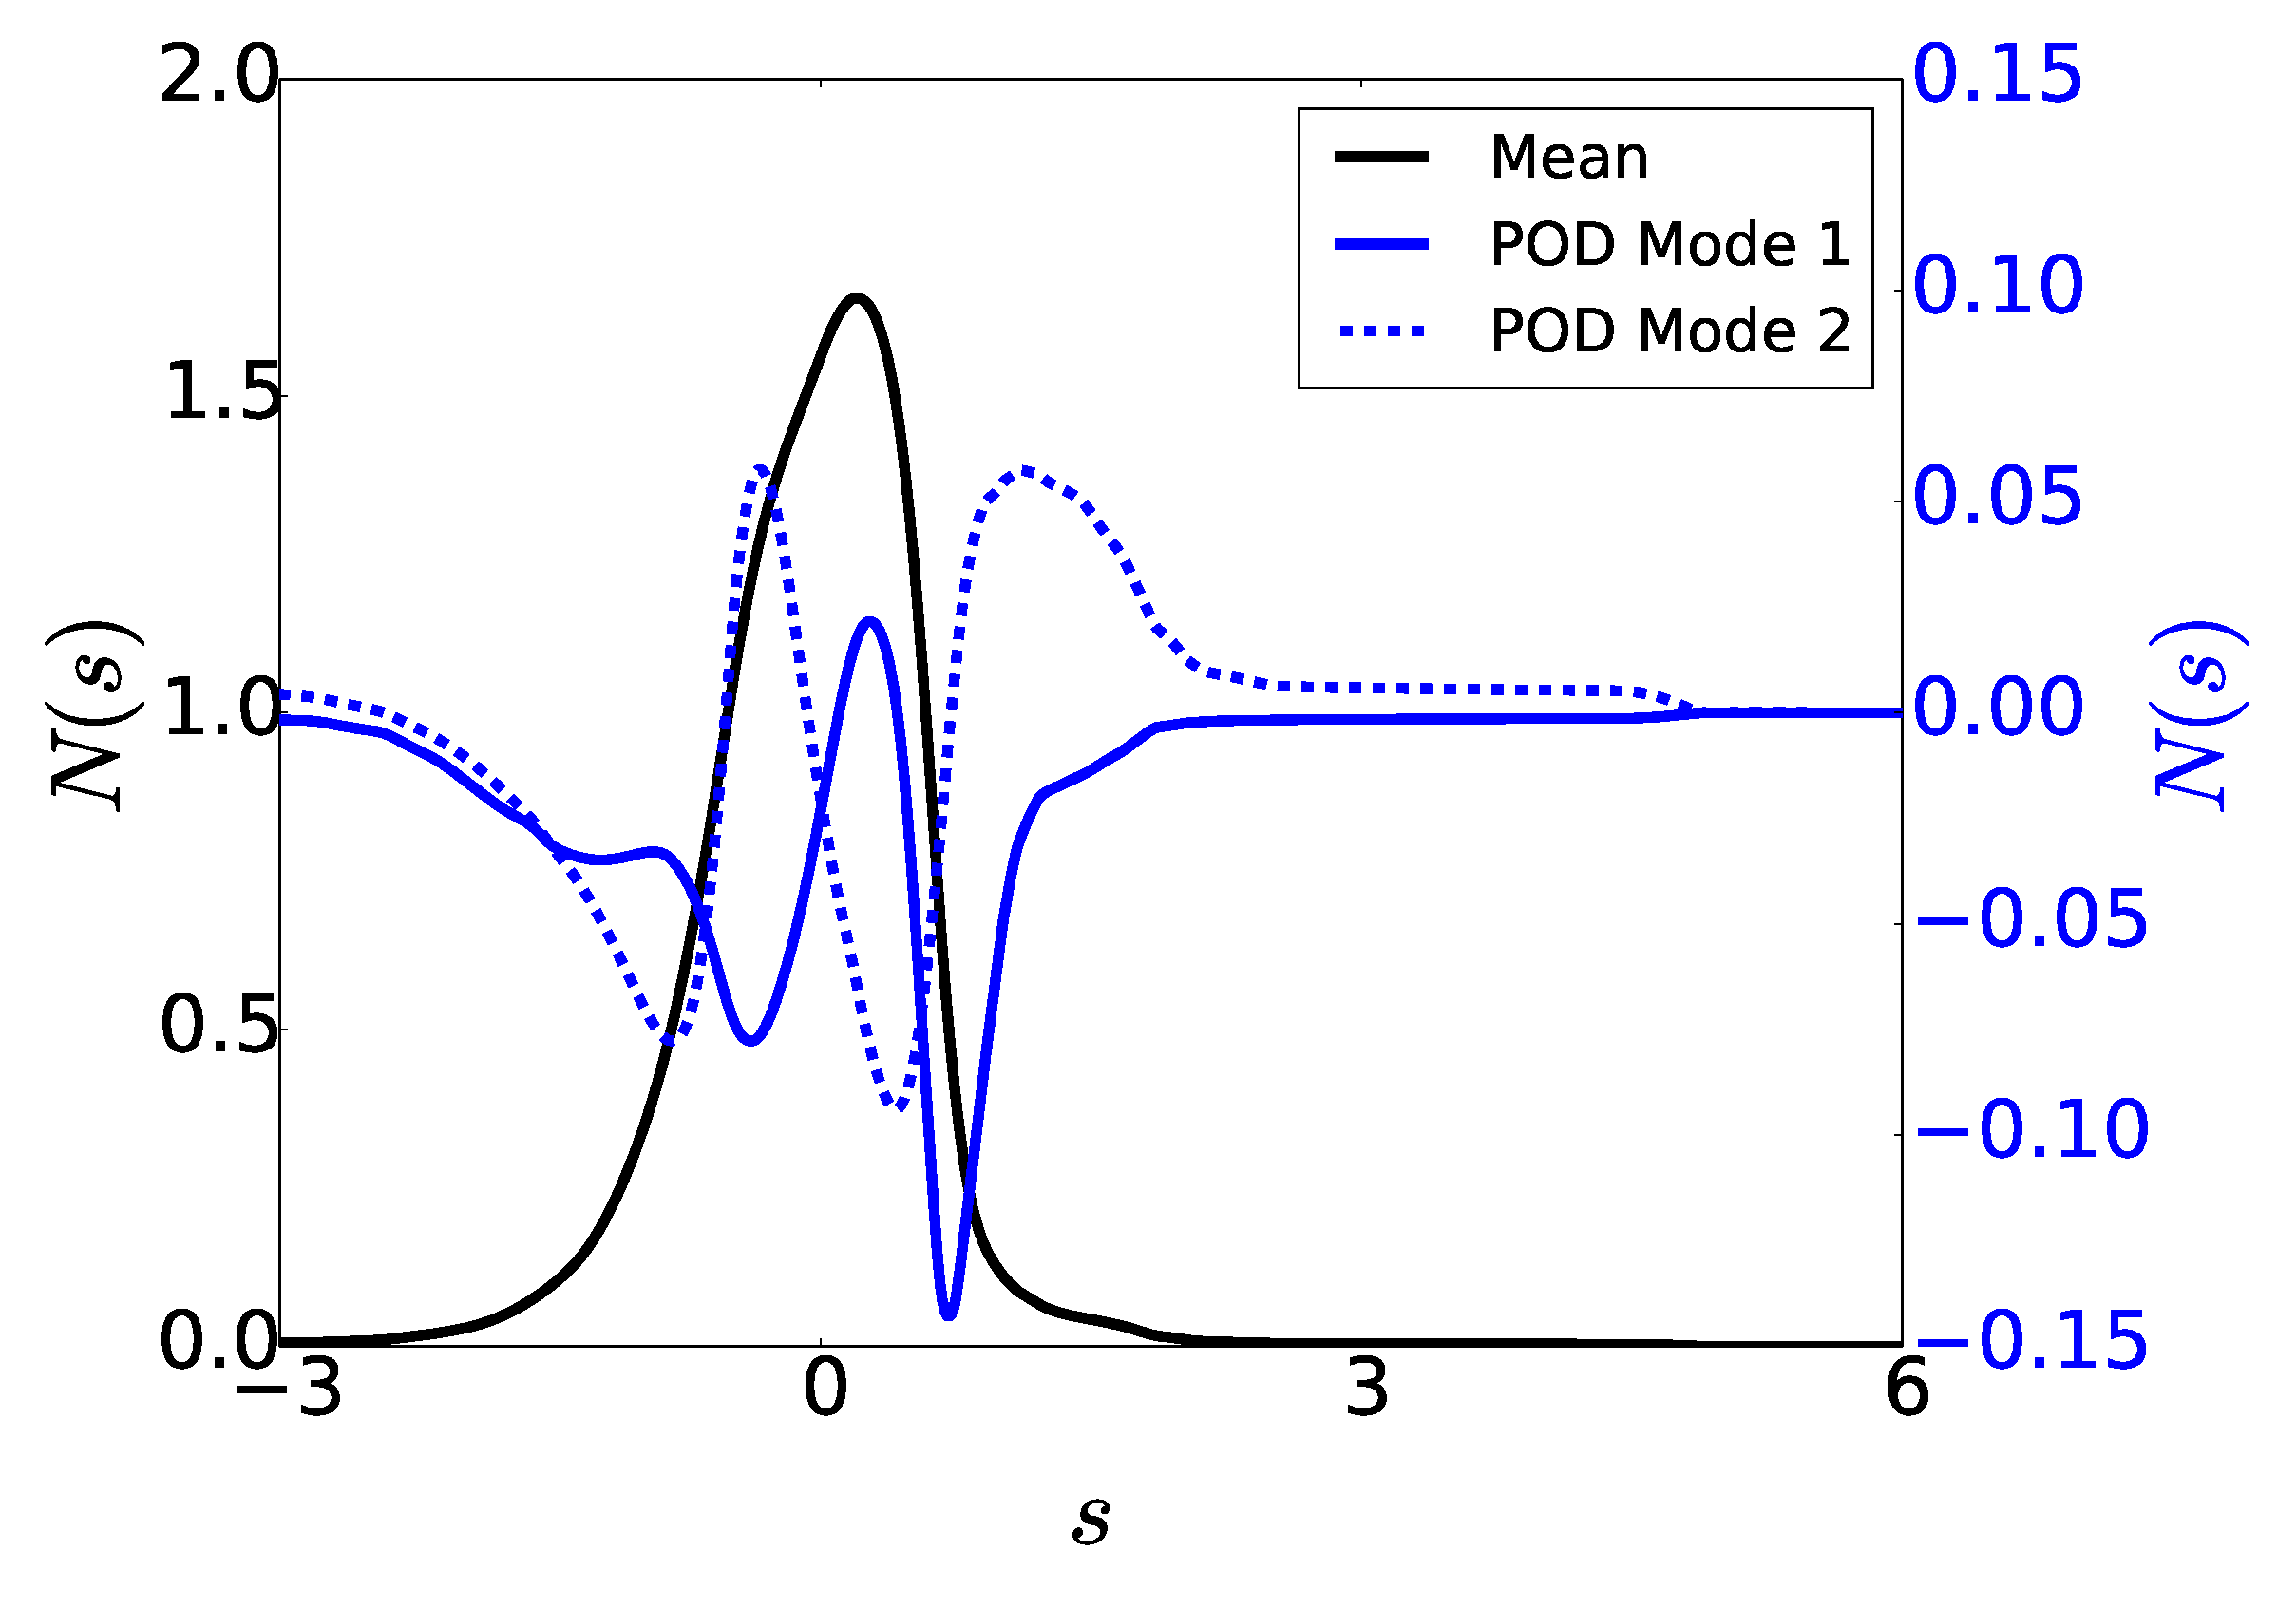
\includegraphics[width=1.25\textwidth]{PODModes} \\
    {\bf POD Modes}
\end{columns}
\vspace{1cm}
\begin{equation*}
N(s) = h \lbrace \bar{N}(as + b) + \sum_{i=1}^2 c_i \Phi_i(as + b)   \rbrace
\end{equation*}

\begin{itemize}
\item \emph{h, a, b} are scaling parameters
\item $c_1, c_2$ are POD coefficients
\item This collapses 100 different snapshots into 5 parameters
\end{itemize}
\end{frame}
\begin{frame}
\frametitle{Data-Based Input Processes: 3D Wing}
\label{sec-3-4}


\begin{columns}[c]
  \column{0.5\textwidth}
    \centering
    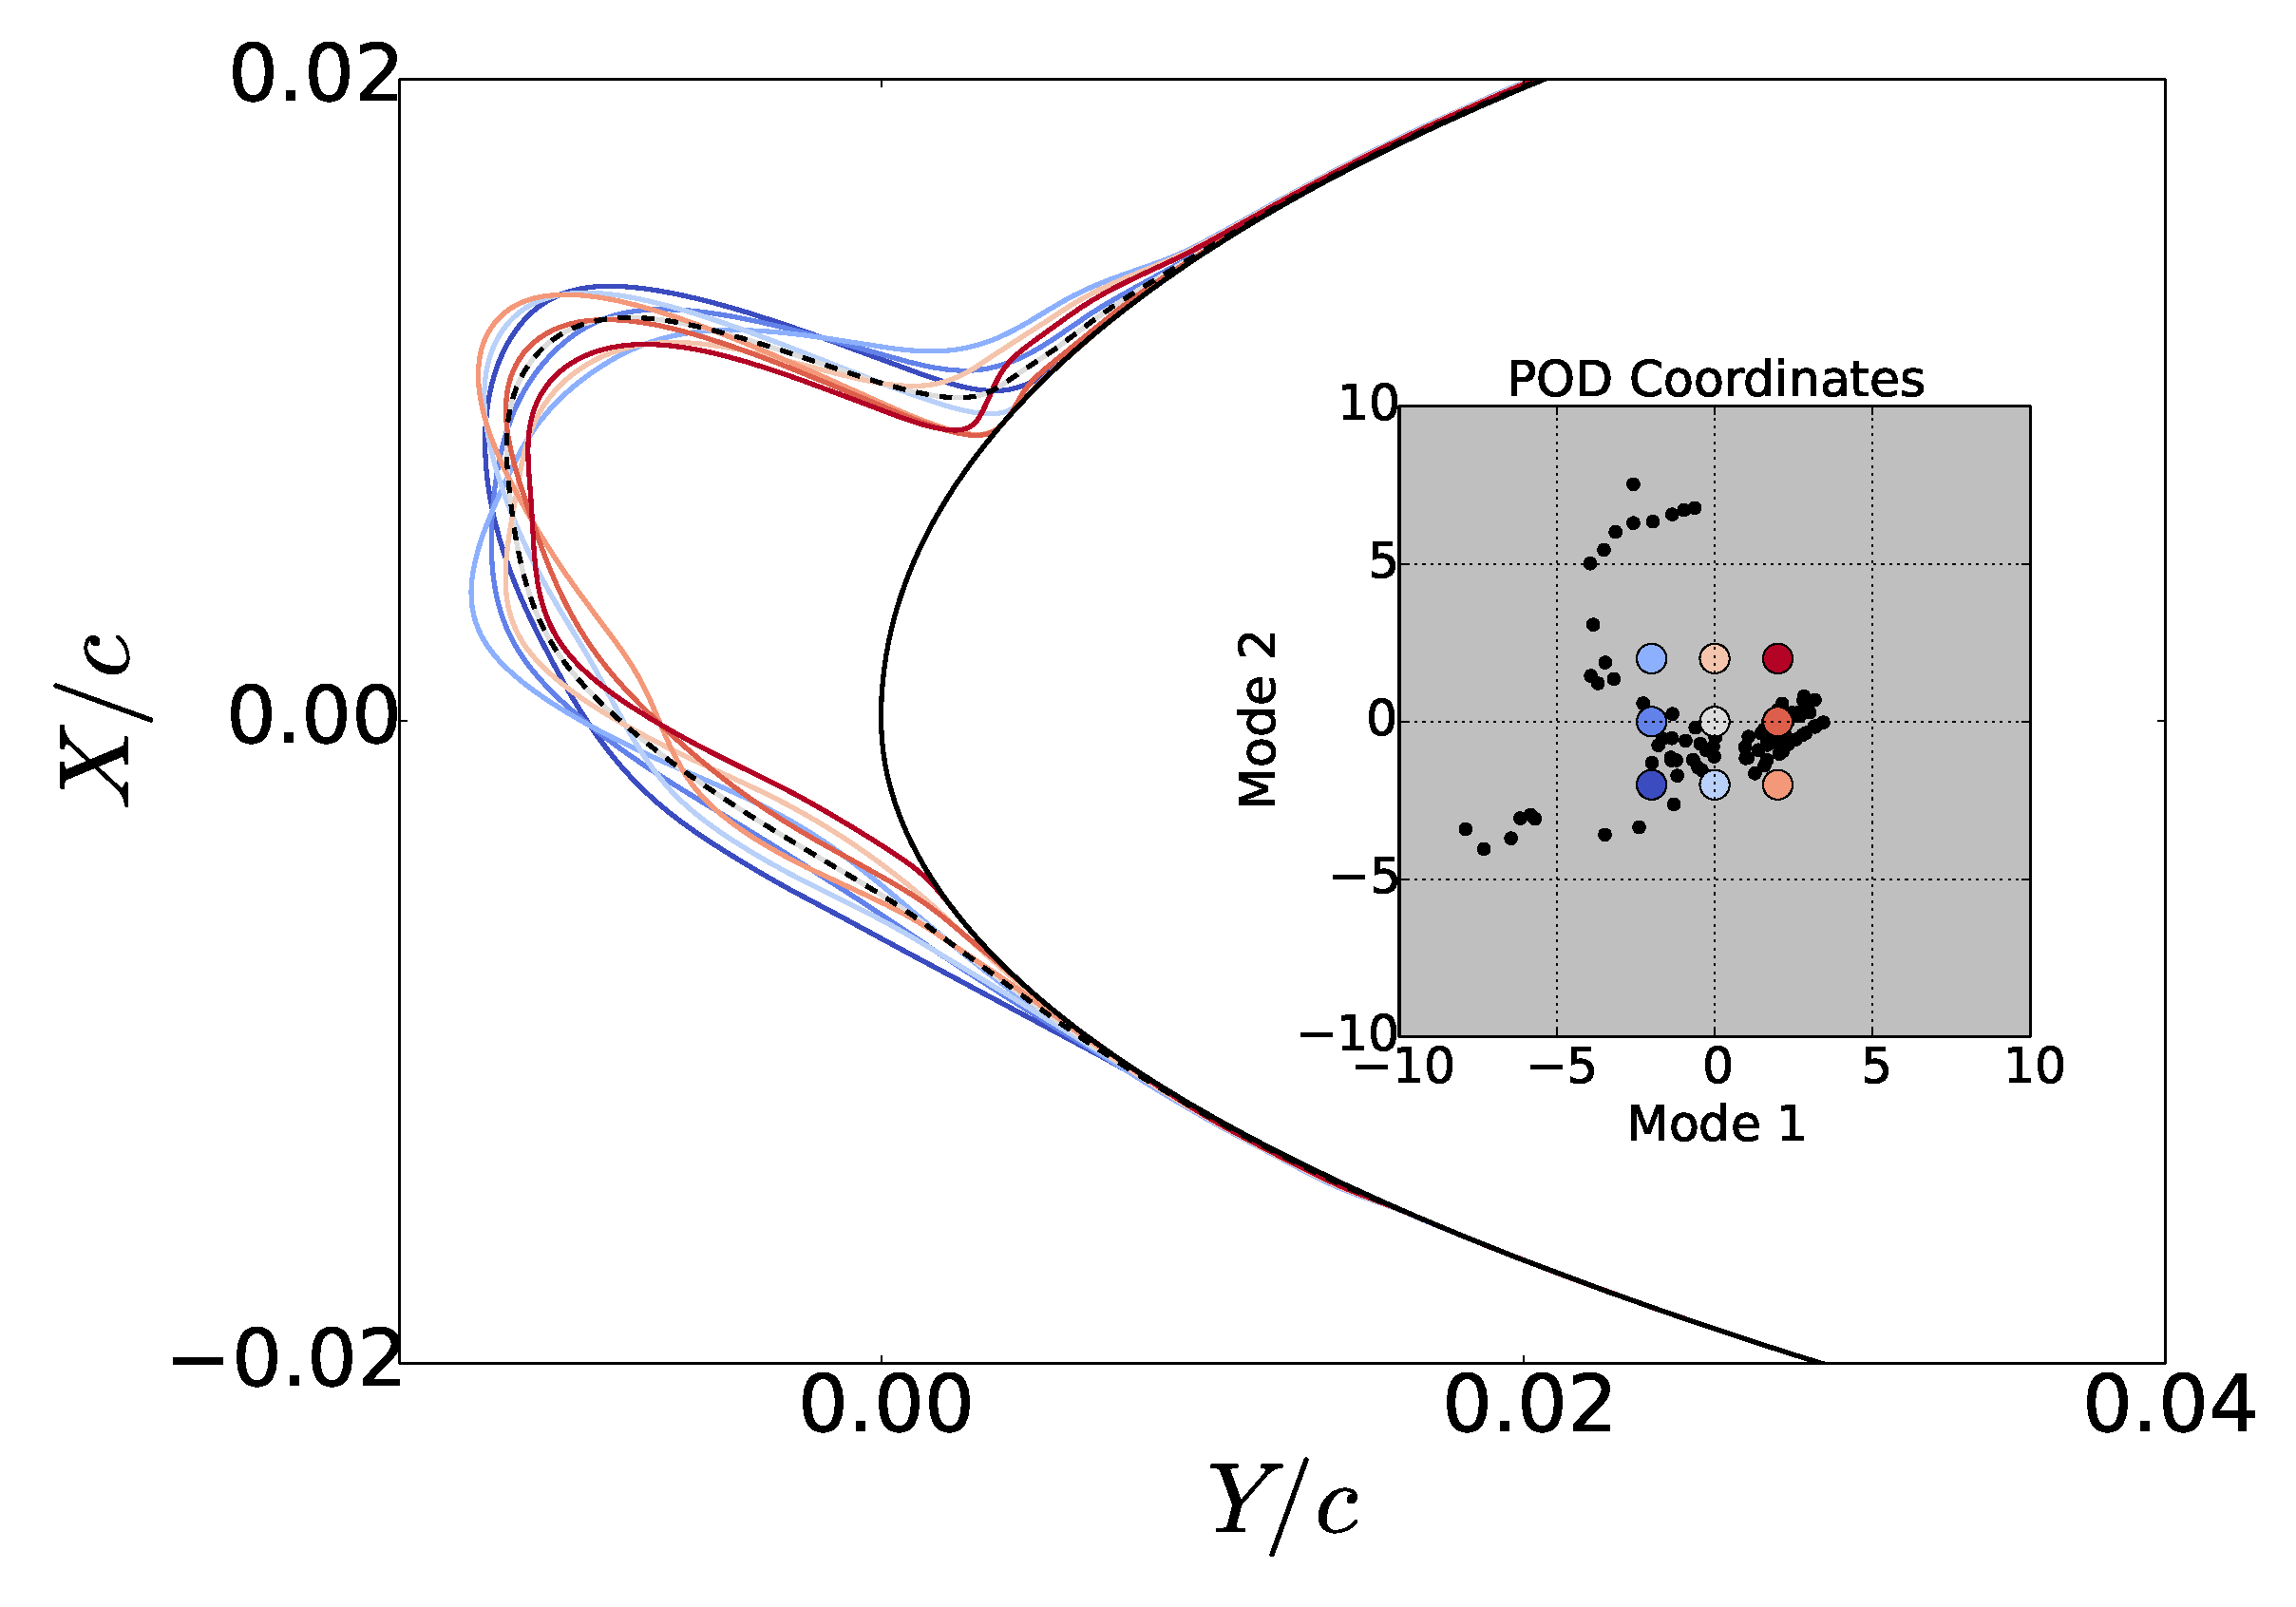
\includegraphics[width=.75\textwidth]{DifferentShapesPODModes} \\
    \bf{POD Modes} \\
    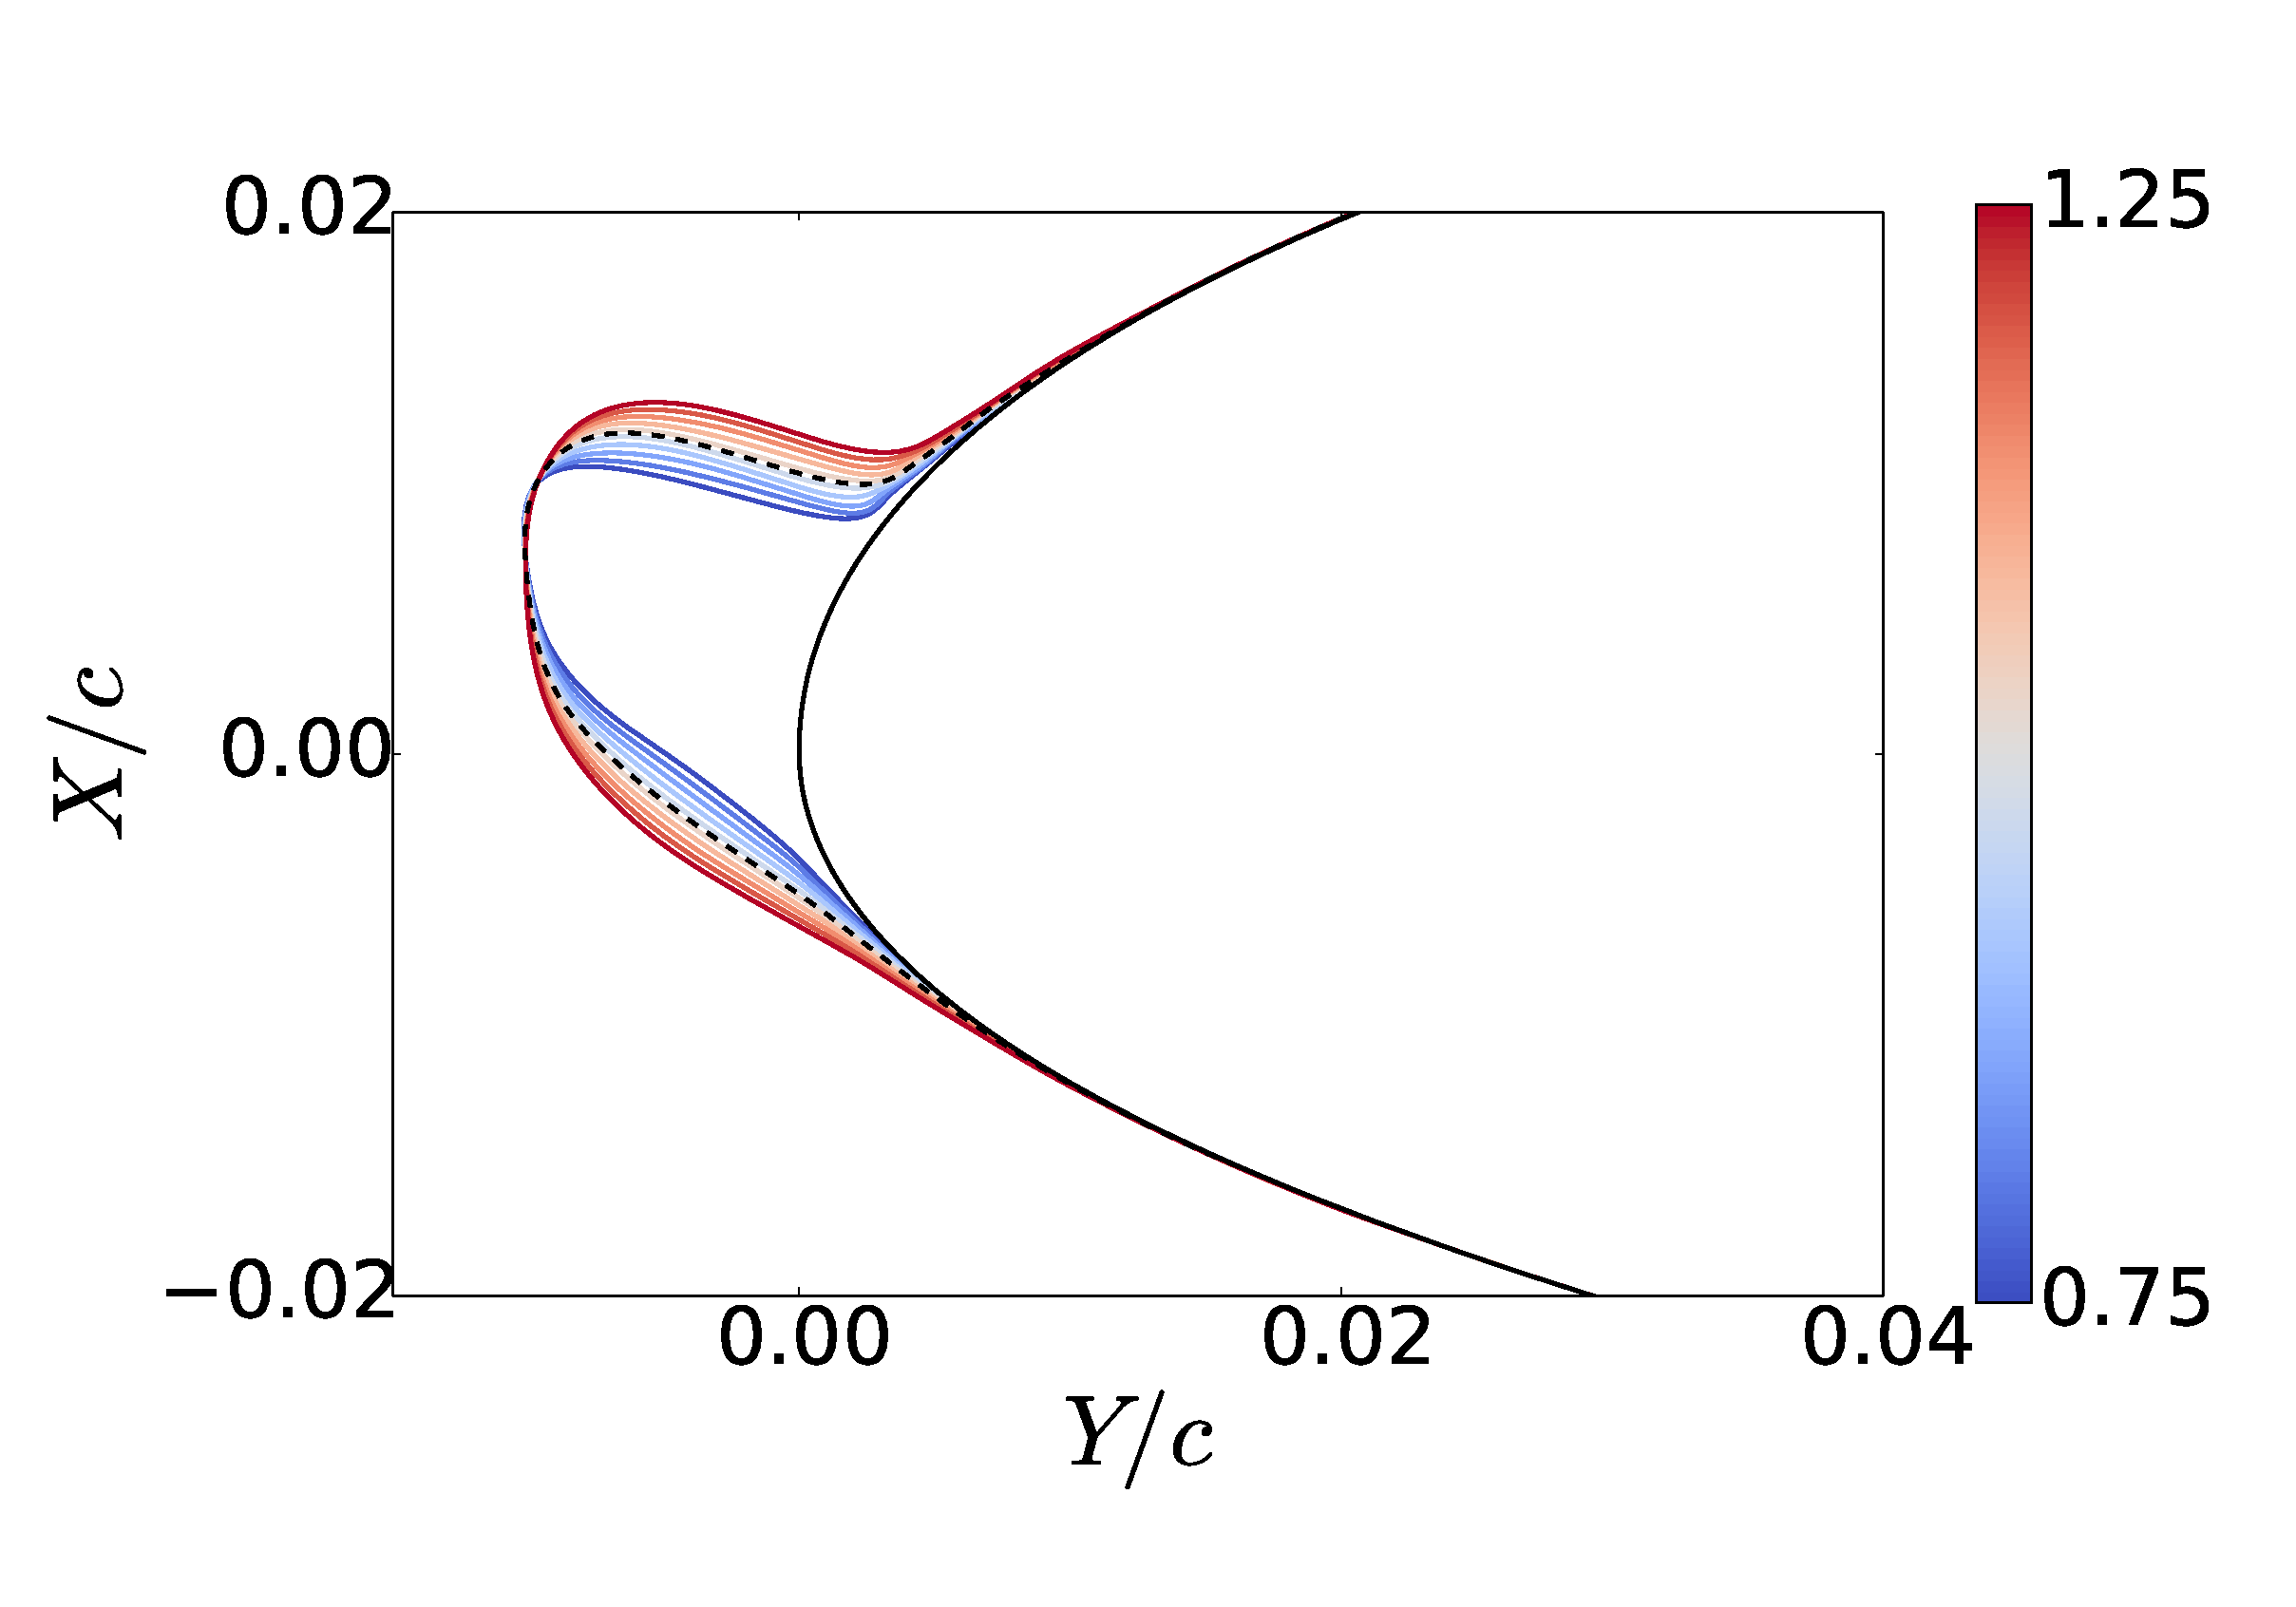
\includegraphics[width=.75\textwidth]{DifferentShapesWidth} \\
    \bf{Width}
  \column{0.5\textwidth}
    \centering
    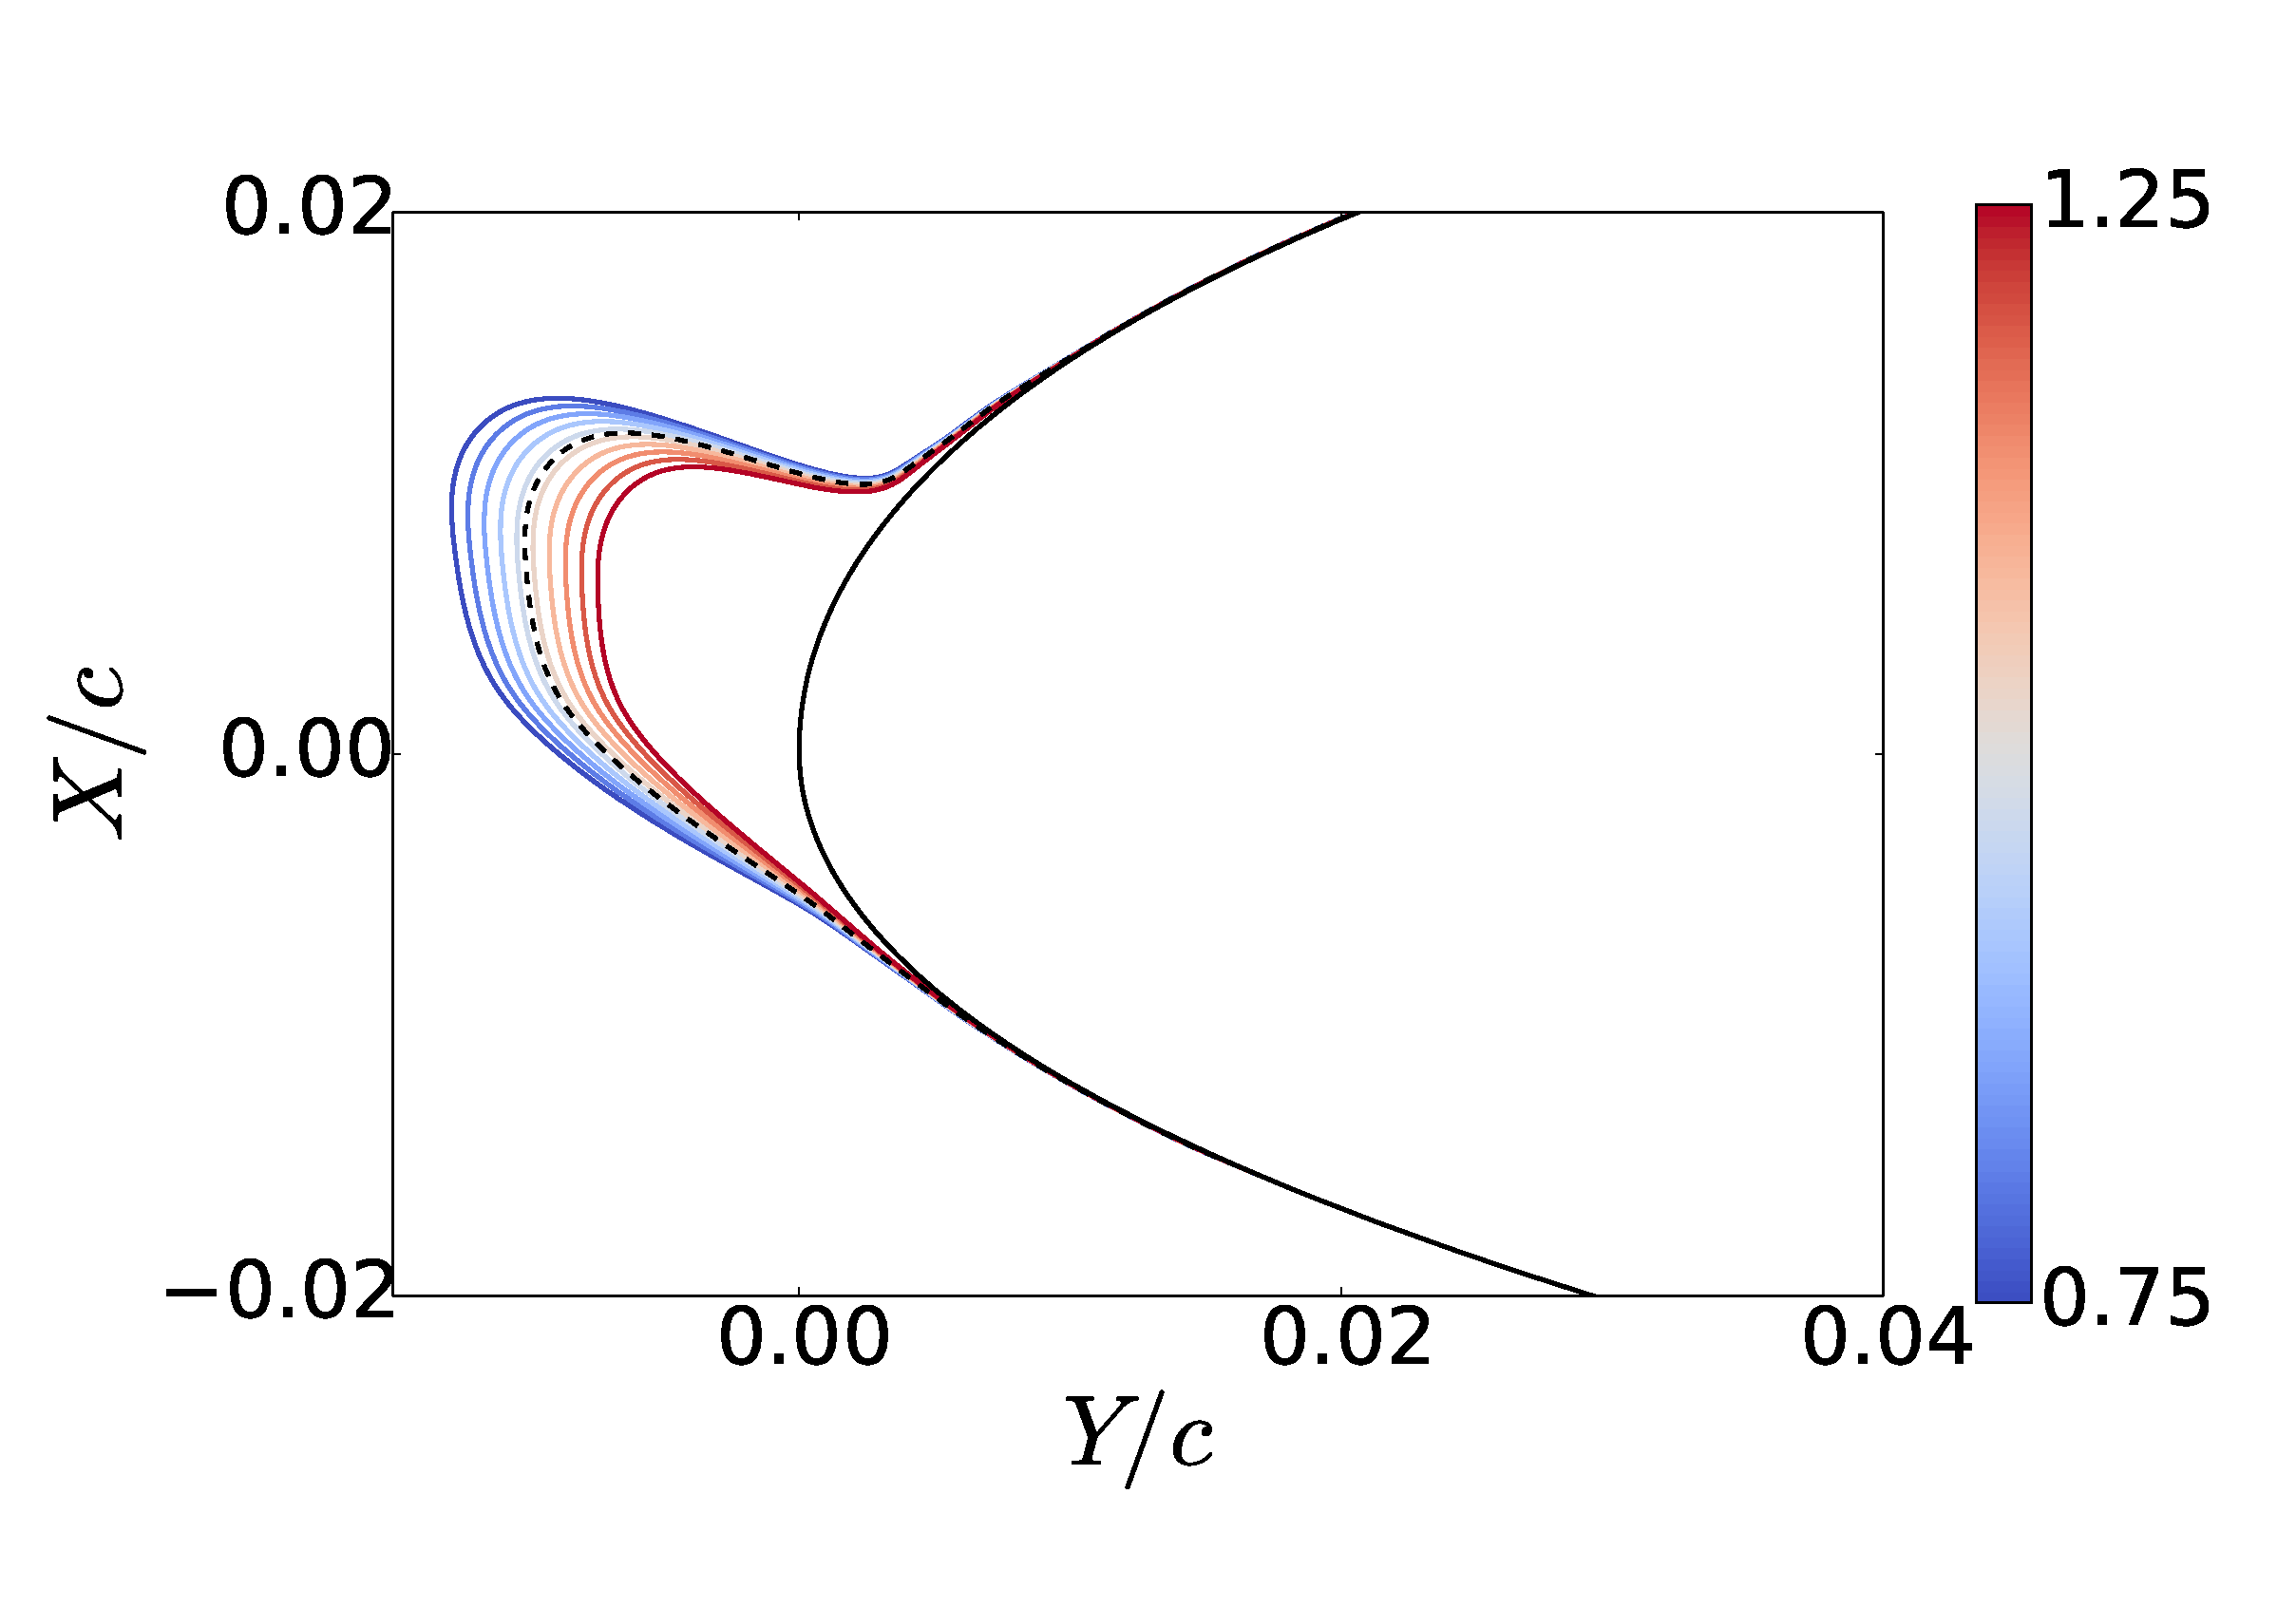
\includegraphics[width=.75\textwidth]{DifferentShapesHeight} \\
    {\bf Height} \\
    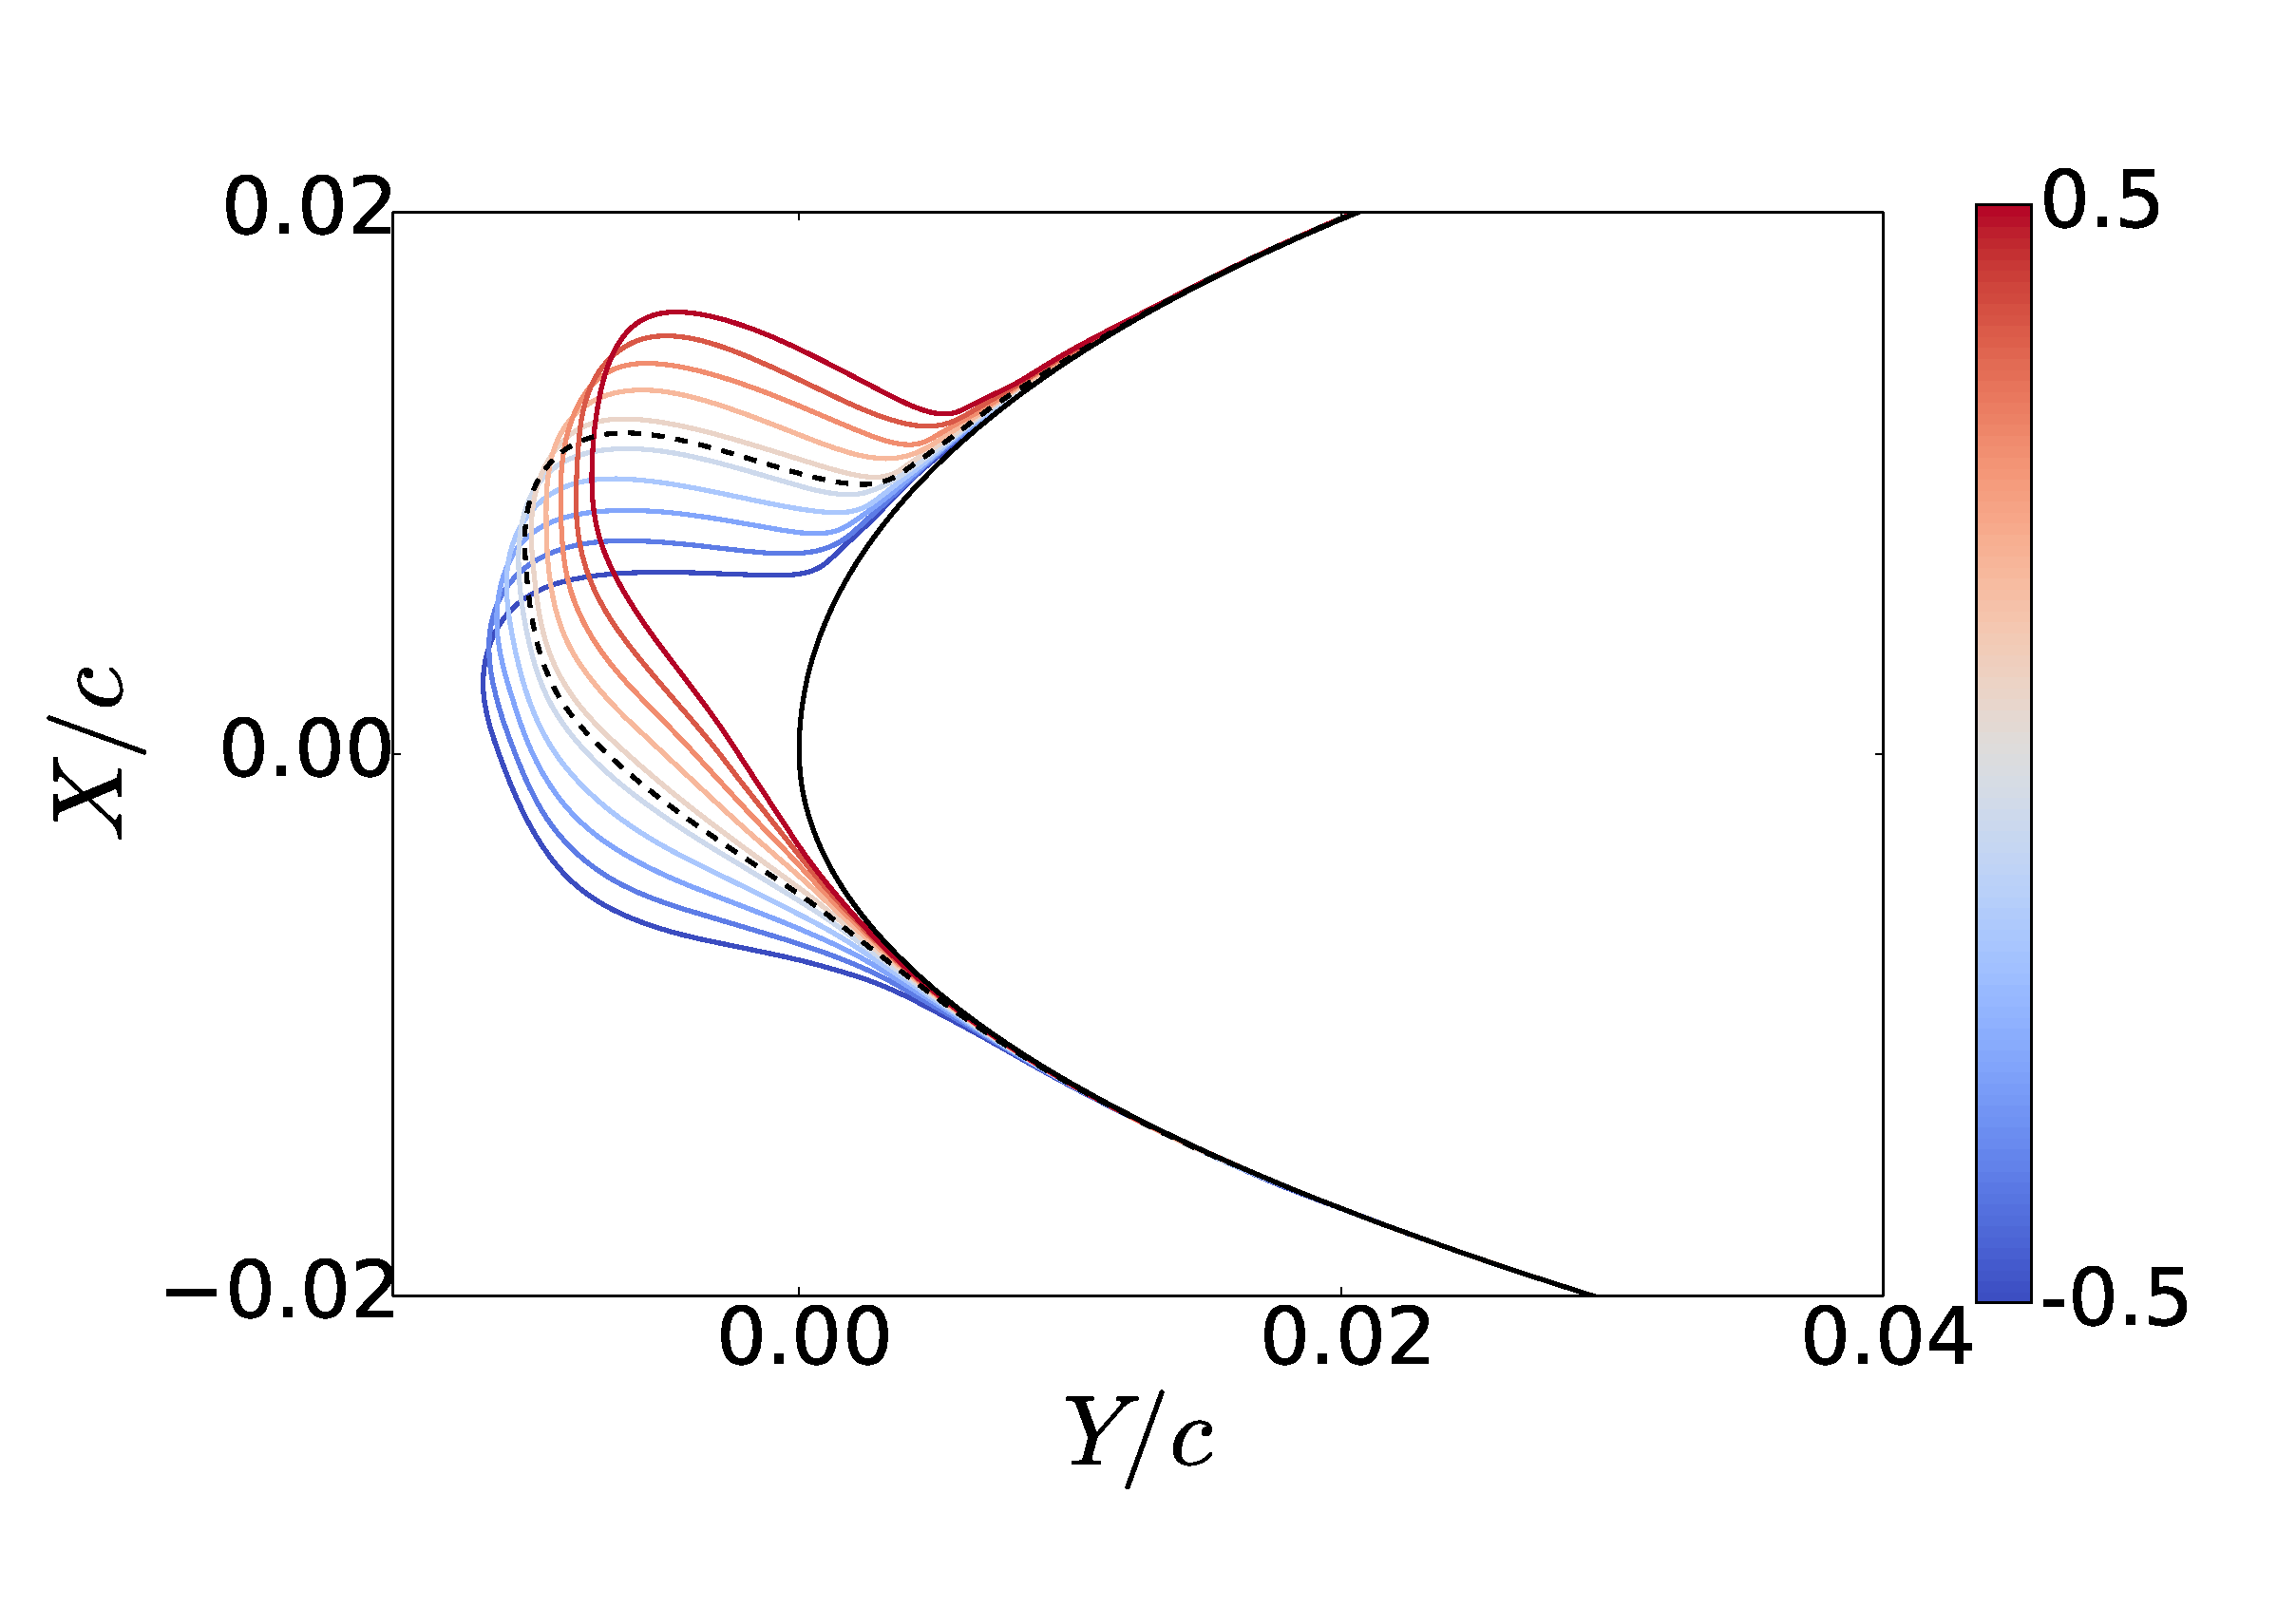
\includegraphics[width=.75\textwidth]{DifferentShapesPosition} \\
    {\bf Position}    
\end{columns}

\begin{itemize}
\item 2 POD coefficients (\emph{shape}) + width, height, position parameters (\emph{scaling})
\end{itemize}
\end{frame}
\begin{frame}
\frametitle{Data-Based Input Processes: 2D Shapes}
\label{sec-3-5}


\begin{figure}
  \centering
  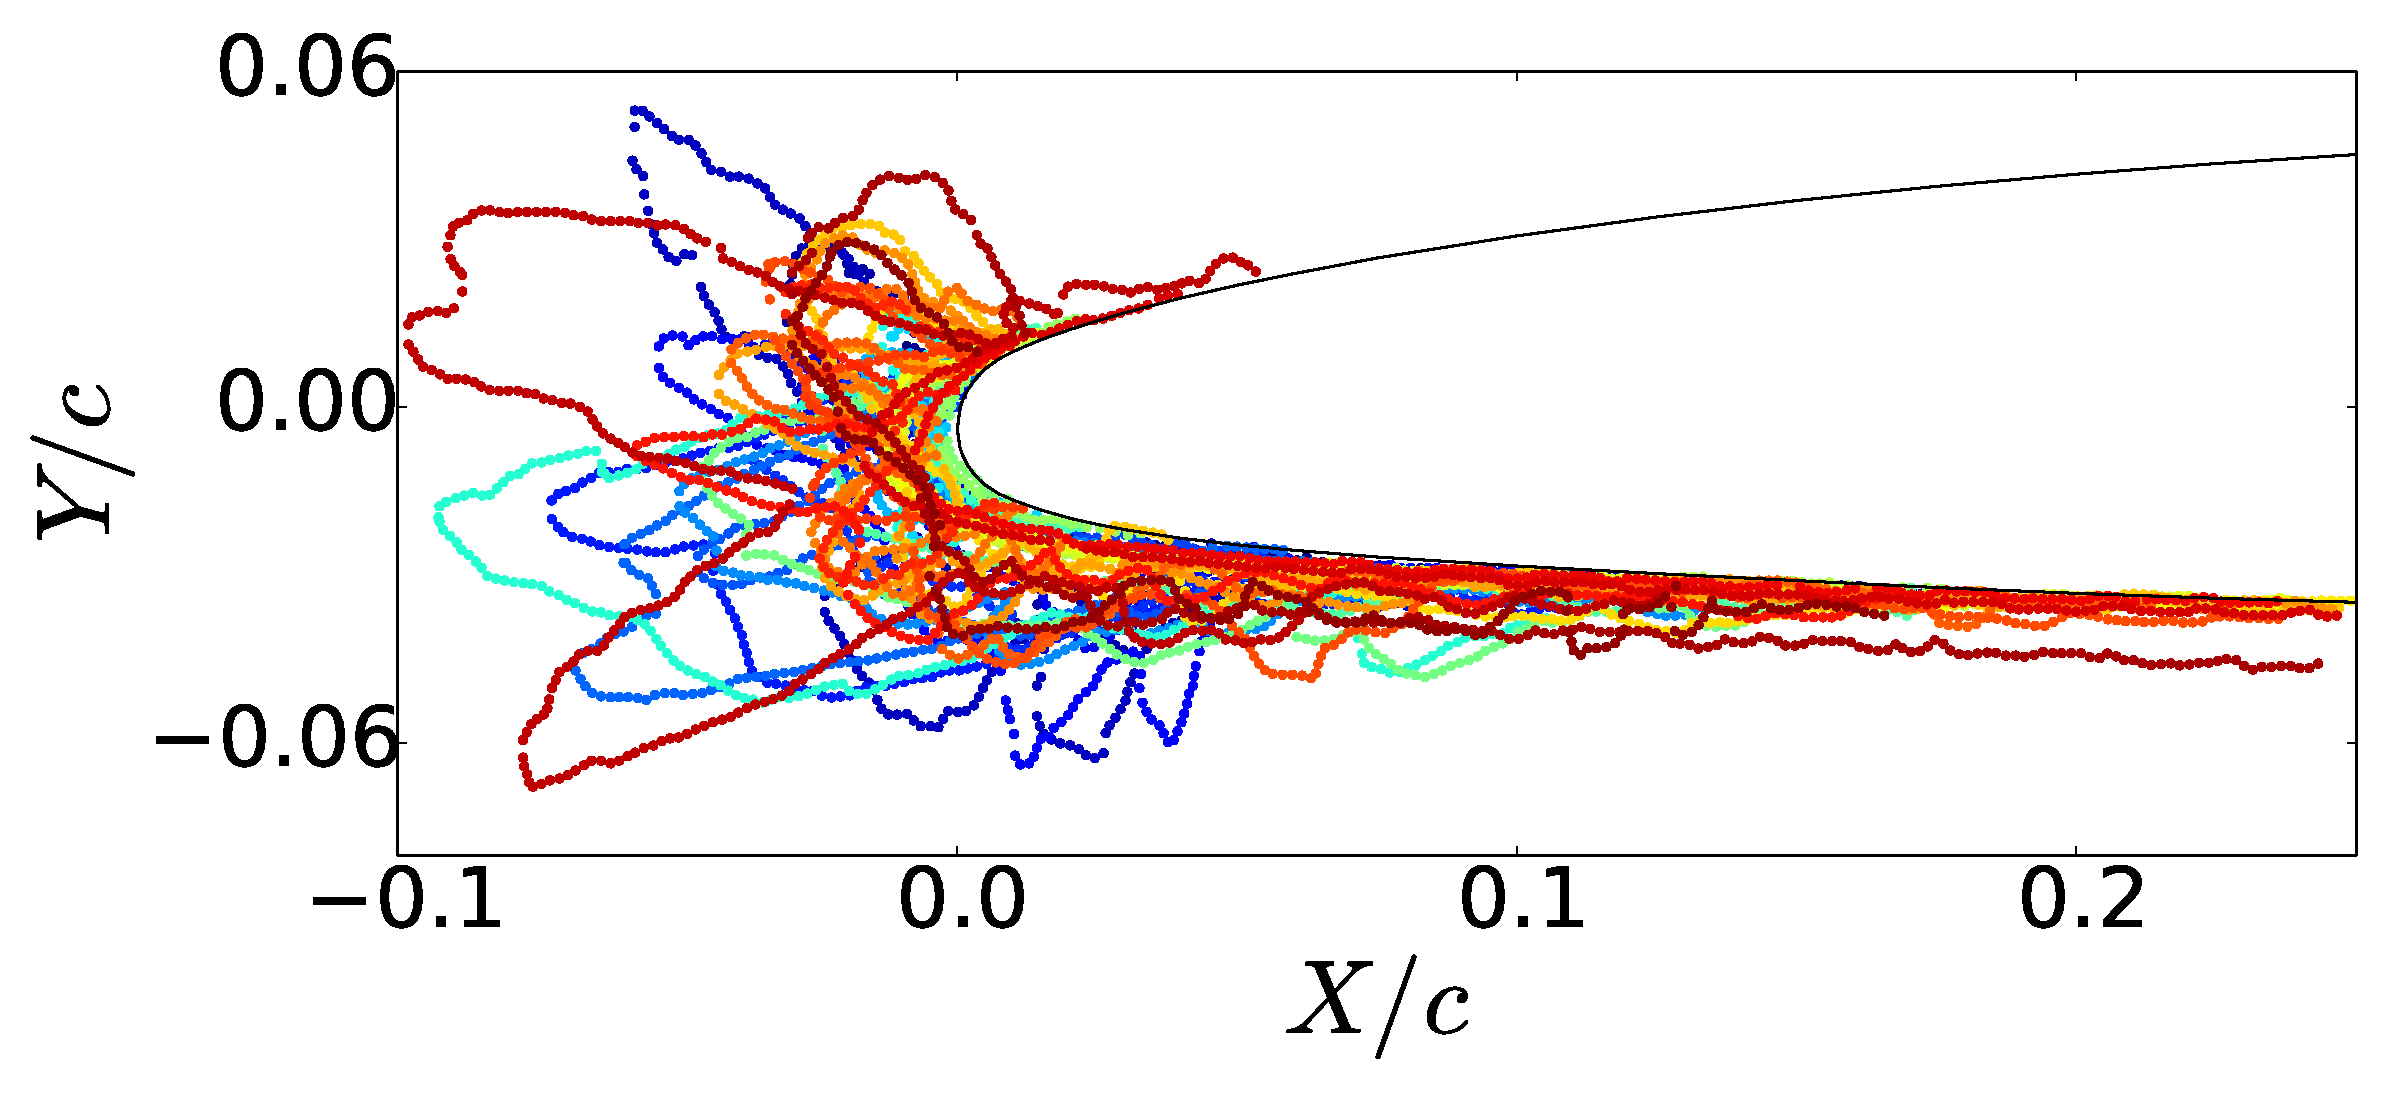
\includegraphics[width=0.7\textwidth]{Dataset}
\end{figure}

\begin{itemize}
\item Business jet clean airfoil geometry\footnote{Addy, H.E. \emph{Ice Accretions and Icing Effects for Modern Airfoils}. NASA TR 2000-210031.
 }
\item 54 ice shapes, exposed to wide range of various icing conditions
  consistent with FAA certification guidelines
\item POD dataset will consist of binary values defined on a static
  Cartesian mesh (`1' if mesh point is on the ice, `0' if not)
\end{itemize}
\end{frame}
\begin{frame}
\frametitle{Data-Based Input Processes: 2D Shapes}
\label{sec-3-6}


\begin{columns}[c]
  \column{0.45\textwidth}
    \centering
    \hspace{-2.17em}
    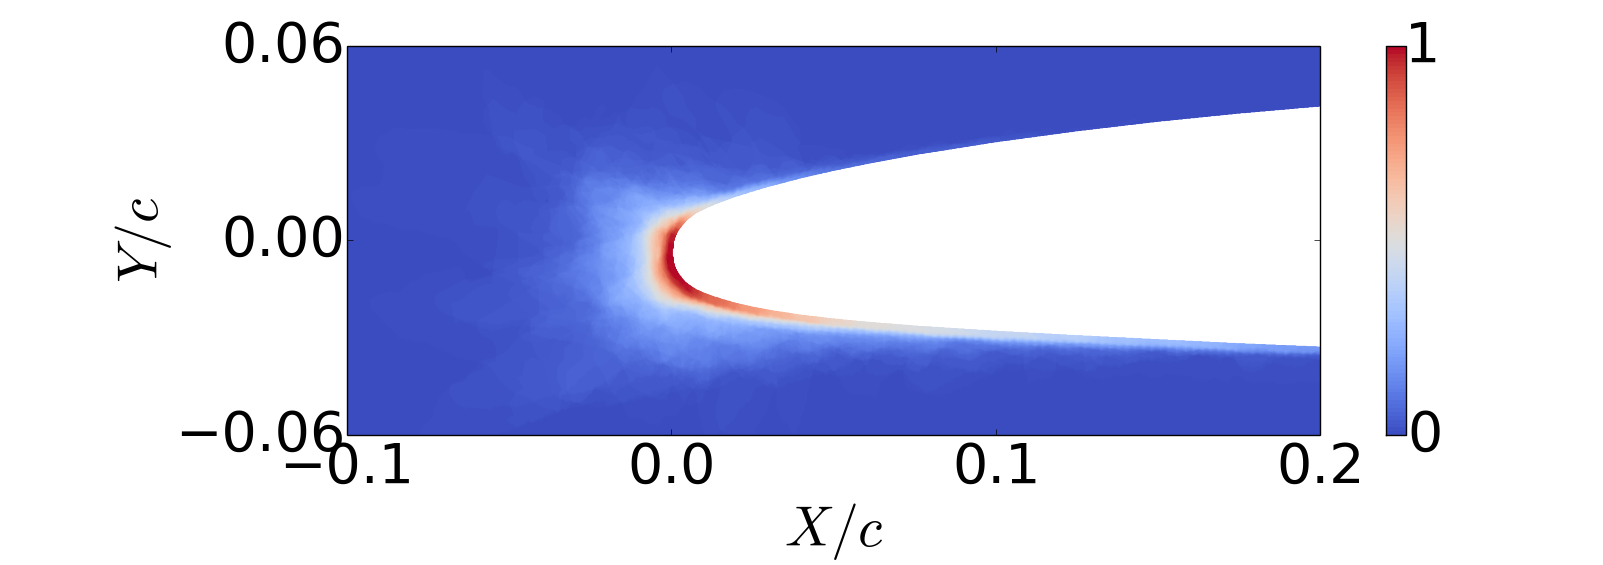
\includegraphics[width=0.9\textwidth]{MEAN.png} \\
    {\bf Mean} \\
    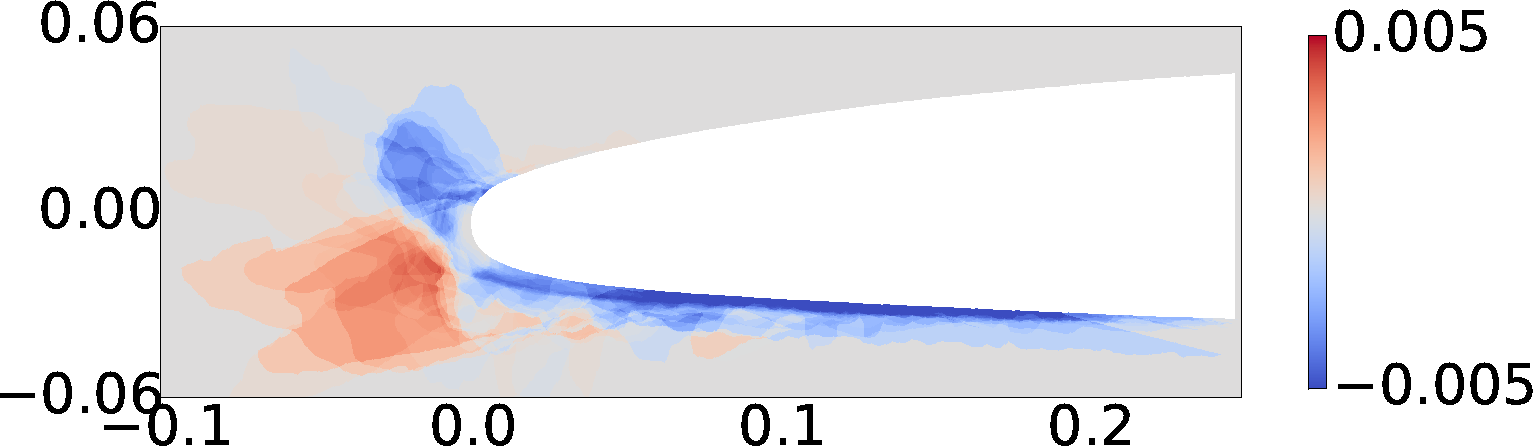
\includegraphics[width=1\textwidth]{MODE2.png} \\
    {\bf Mode 2} \\
    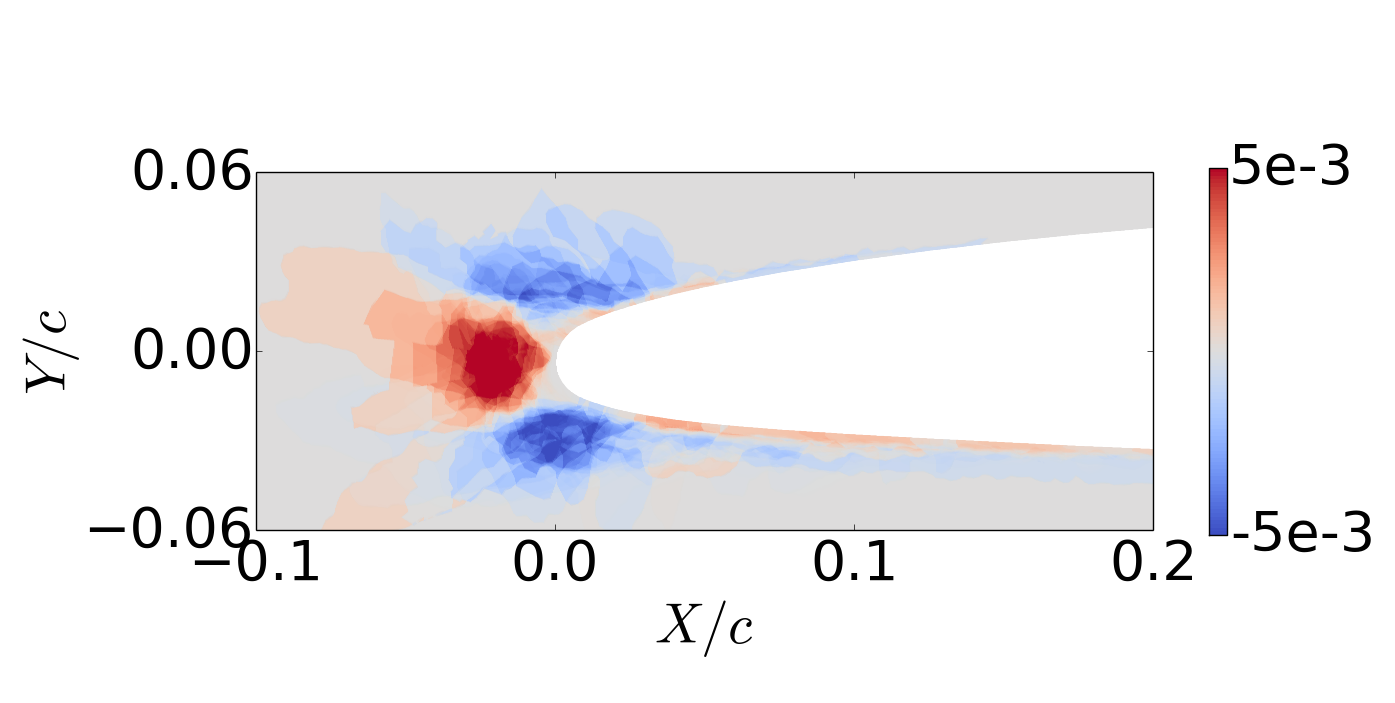
\includegraphics[width=1\textwidth]{MODE4.png} \\
    {\bf Mode 4}
  \column{0.45\textwidth}
    \centering
    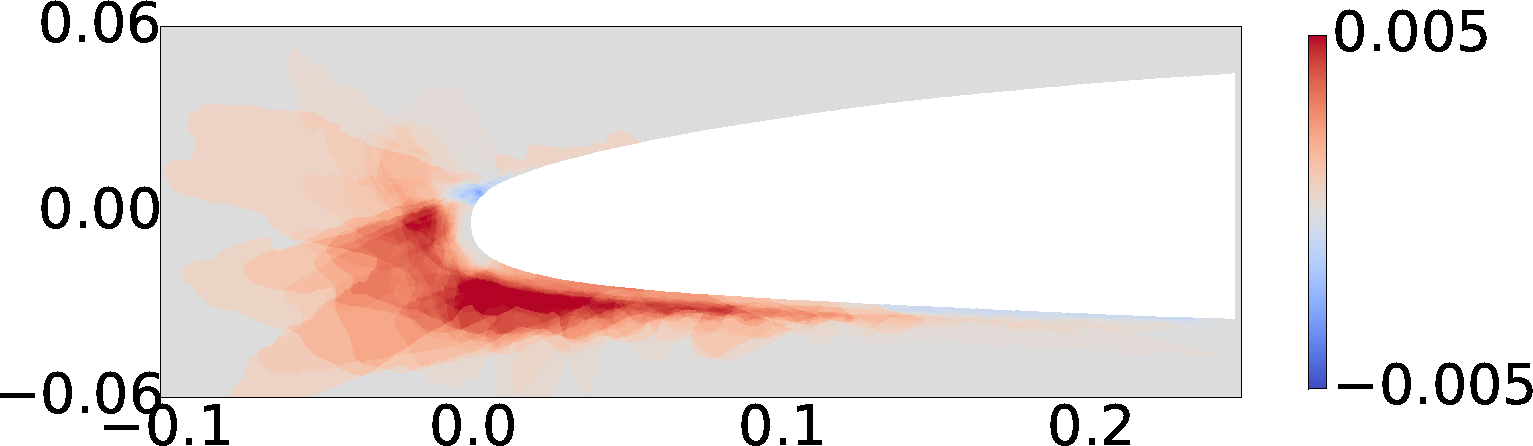
\includegraphics[width=1\textwidth]{MODE1.png} \\
    {\bf Mode 1} \\
    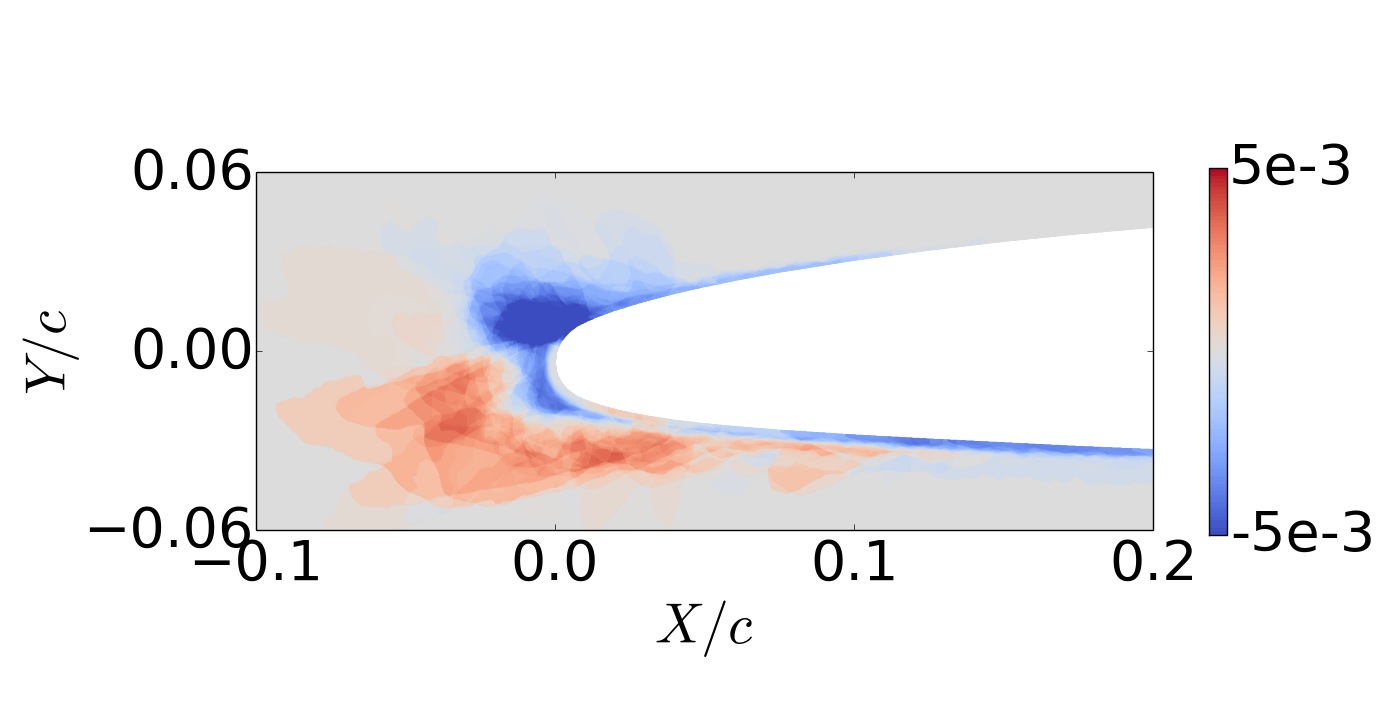
\includegraphics[width=1\textwidth]{MODE3.png} \\
    {\bf Mode 3} \\
    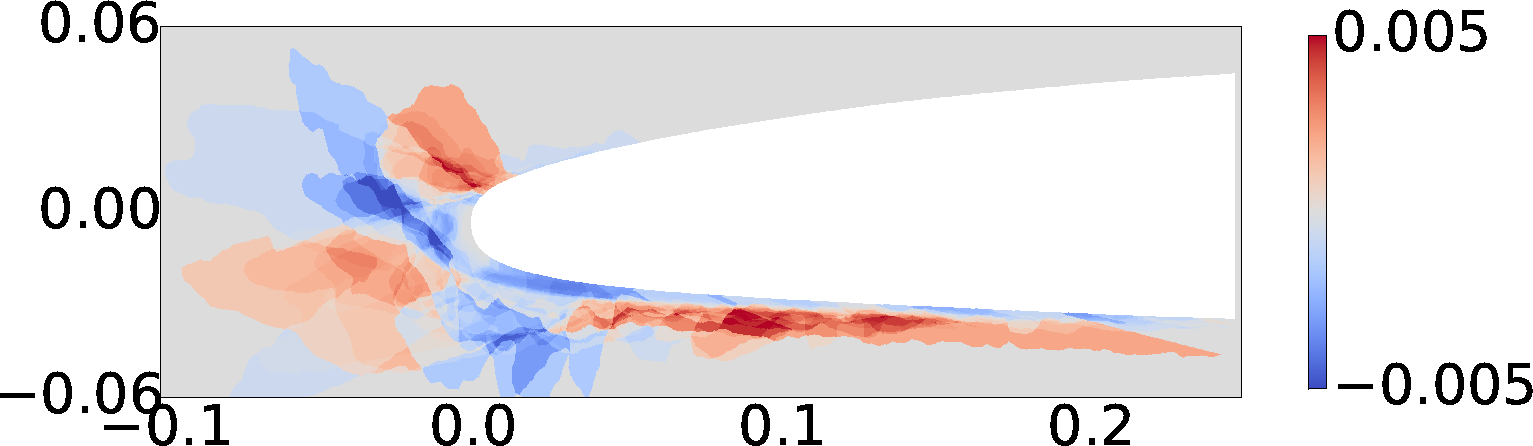
\includegraphics[width=1\textwidth]{MODE5.png} \\
    {\bf Mode 5}
\end{columns}


\begin{itemize}
\item 8 Modes retained; this is where POD eigenvalue magnitudes have
  decayed by an order of magnitude
\end{itemize}
\end{frame}
\begin{frame}
\frametitle{Data-Based Input Processes: 2D Shapes}
\label{sec-3-7}


\begin{columns}[c]
  \column{0.45\textwidth}
    \centering
    \hspace{-0.5em}
    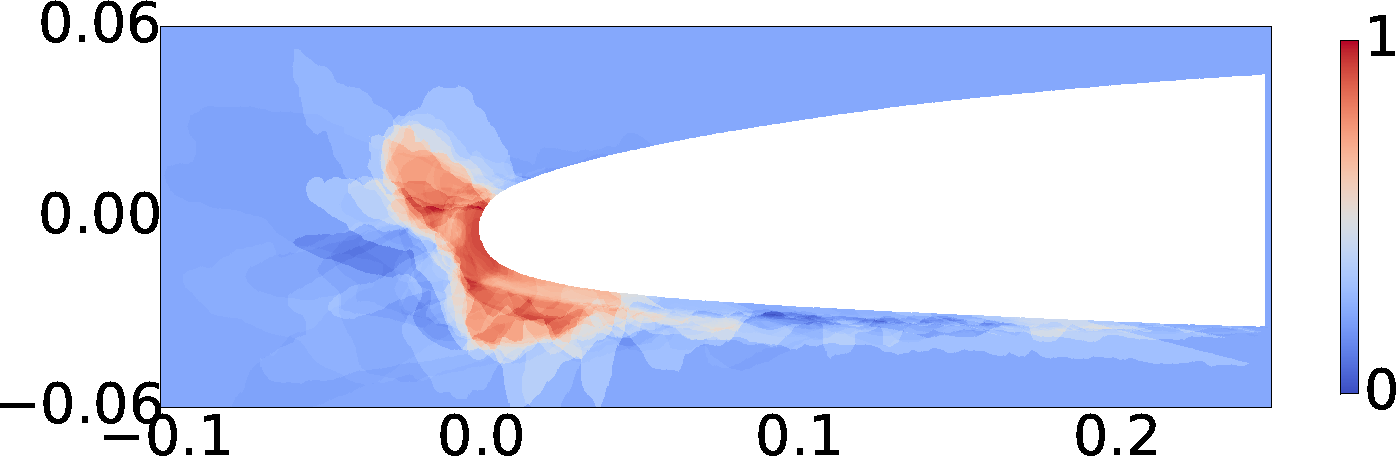
\includegraphics[width=1\textwidth]{UnfilteredReconstruction.png} \\
    {\bf Unfiltered Reconstruction} \\
    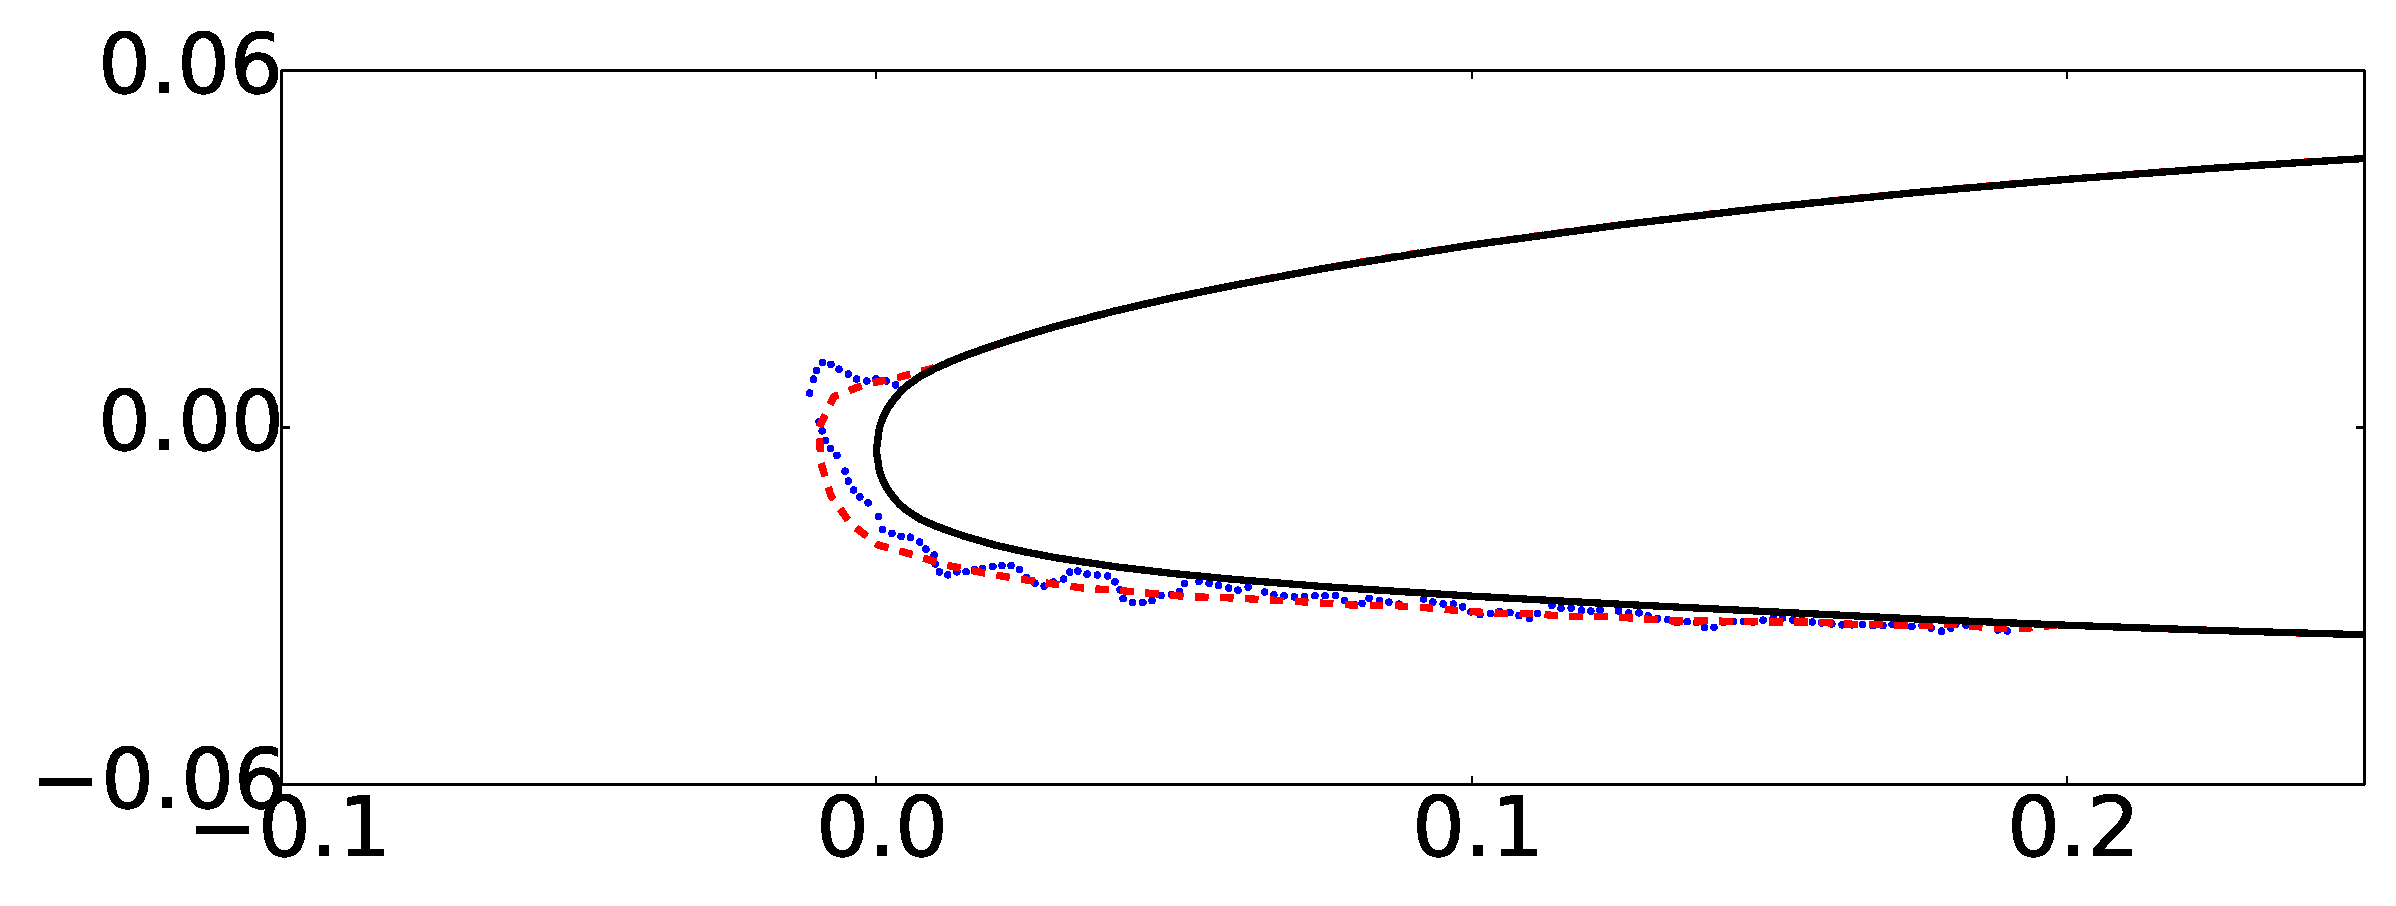
\includegraphics[width=1\textwidth]{ReconstructionE1} \\
    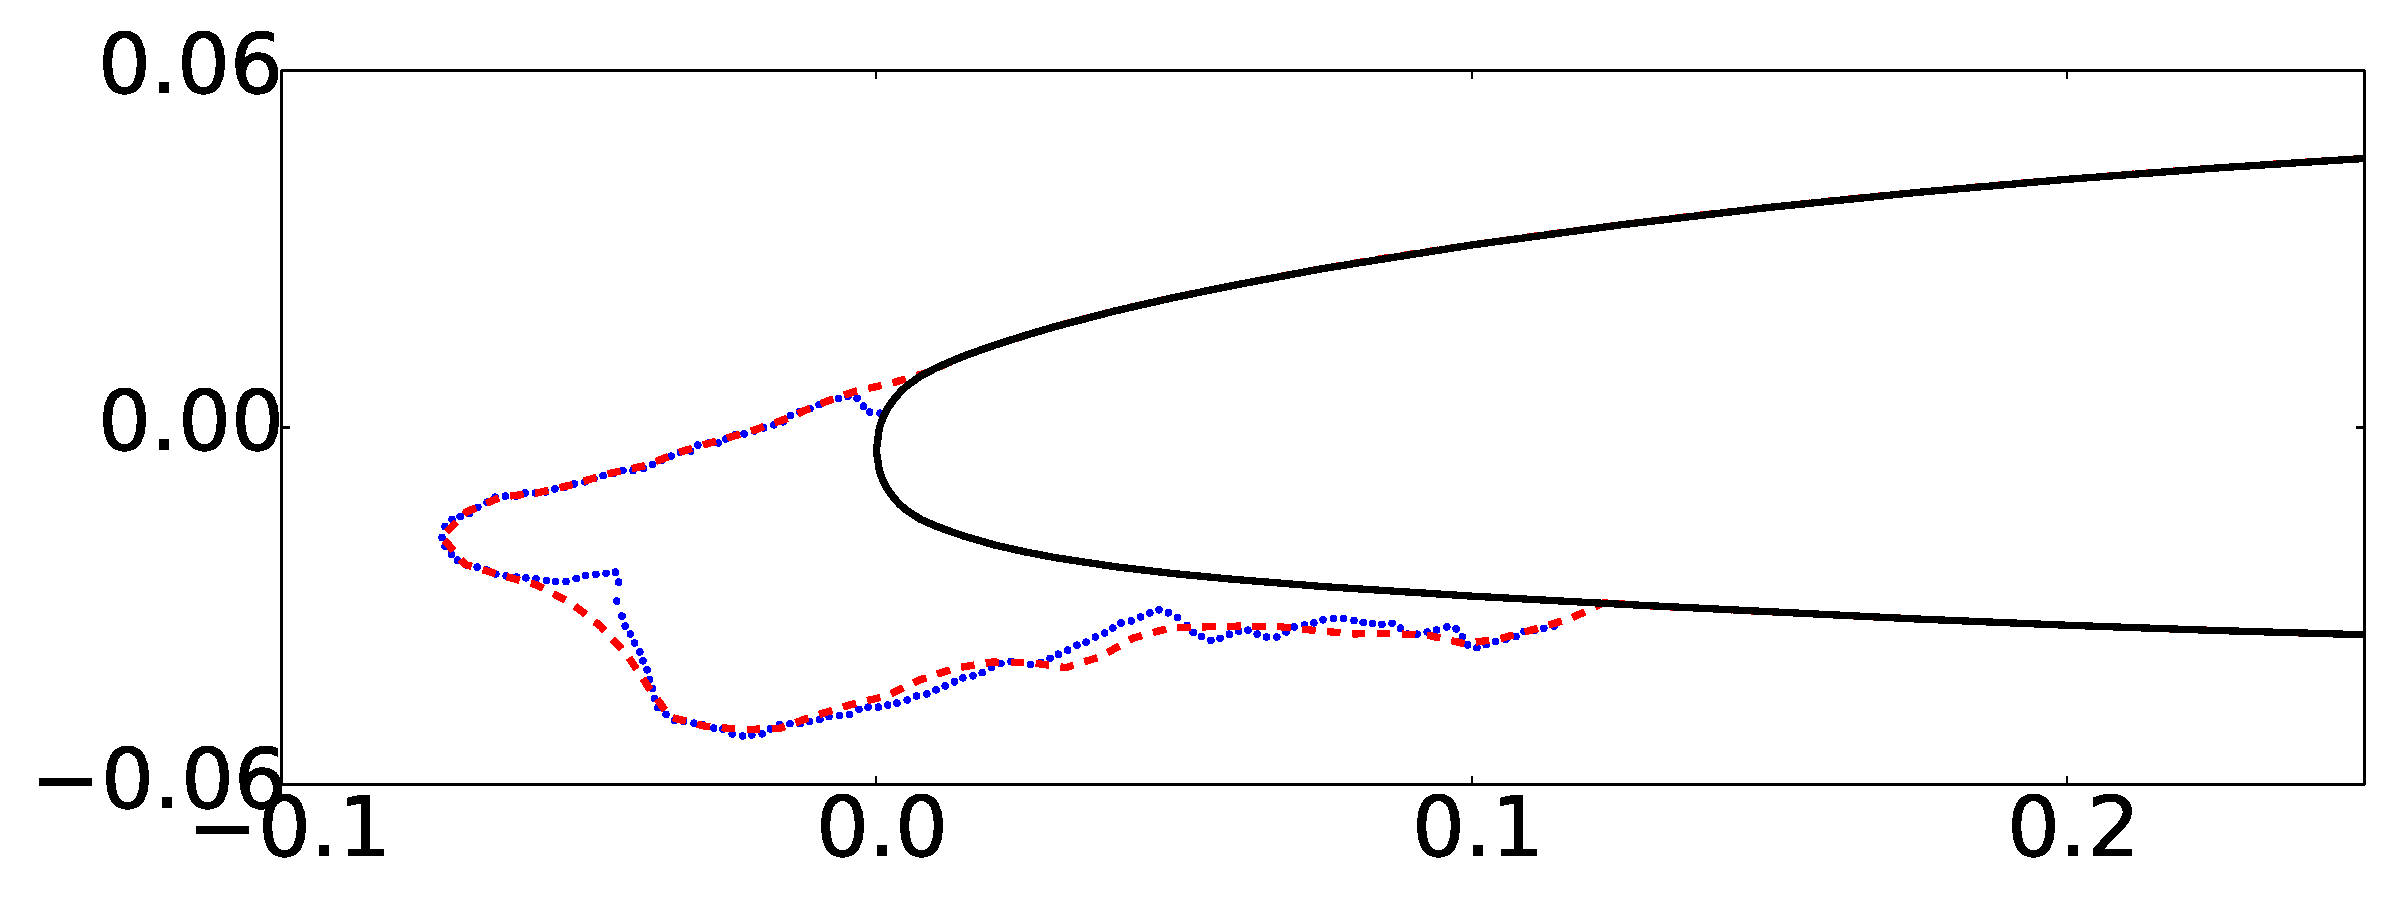
\includegraphics[width=1\textwidth]{ReconstructionE9} \\
  \column{0.45\textwidth}
    \centering
    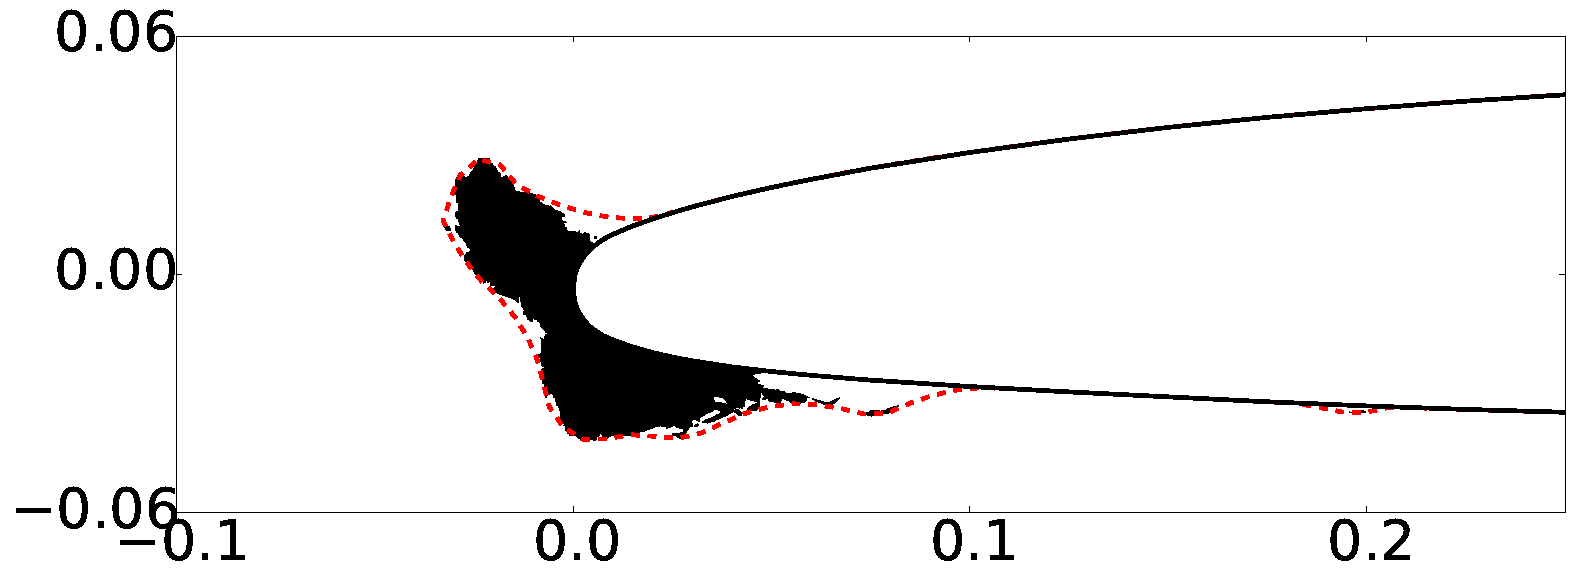
\includegraphics[width=1\textwidth]{FilteredReconstruction.png} \\
    {\bf Filtered Reconstruction} \\
    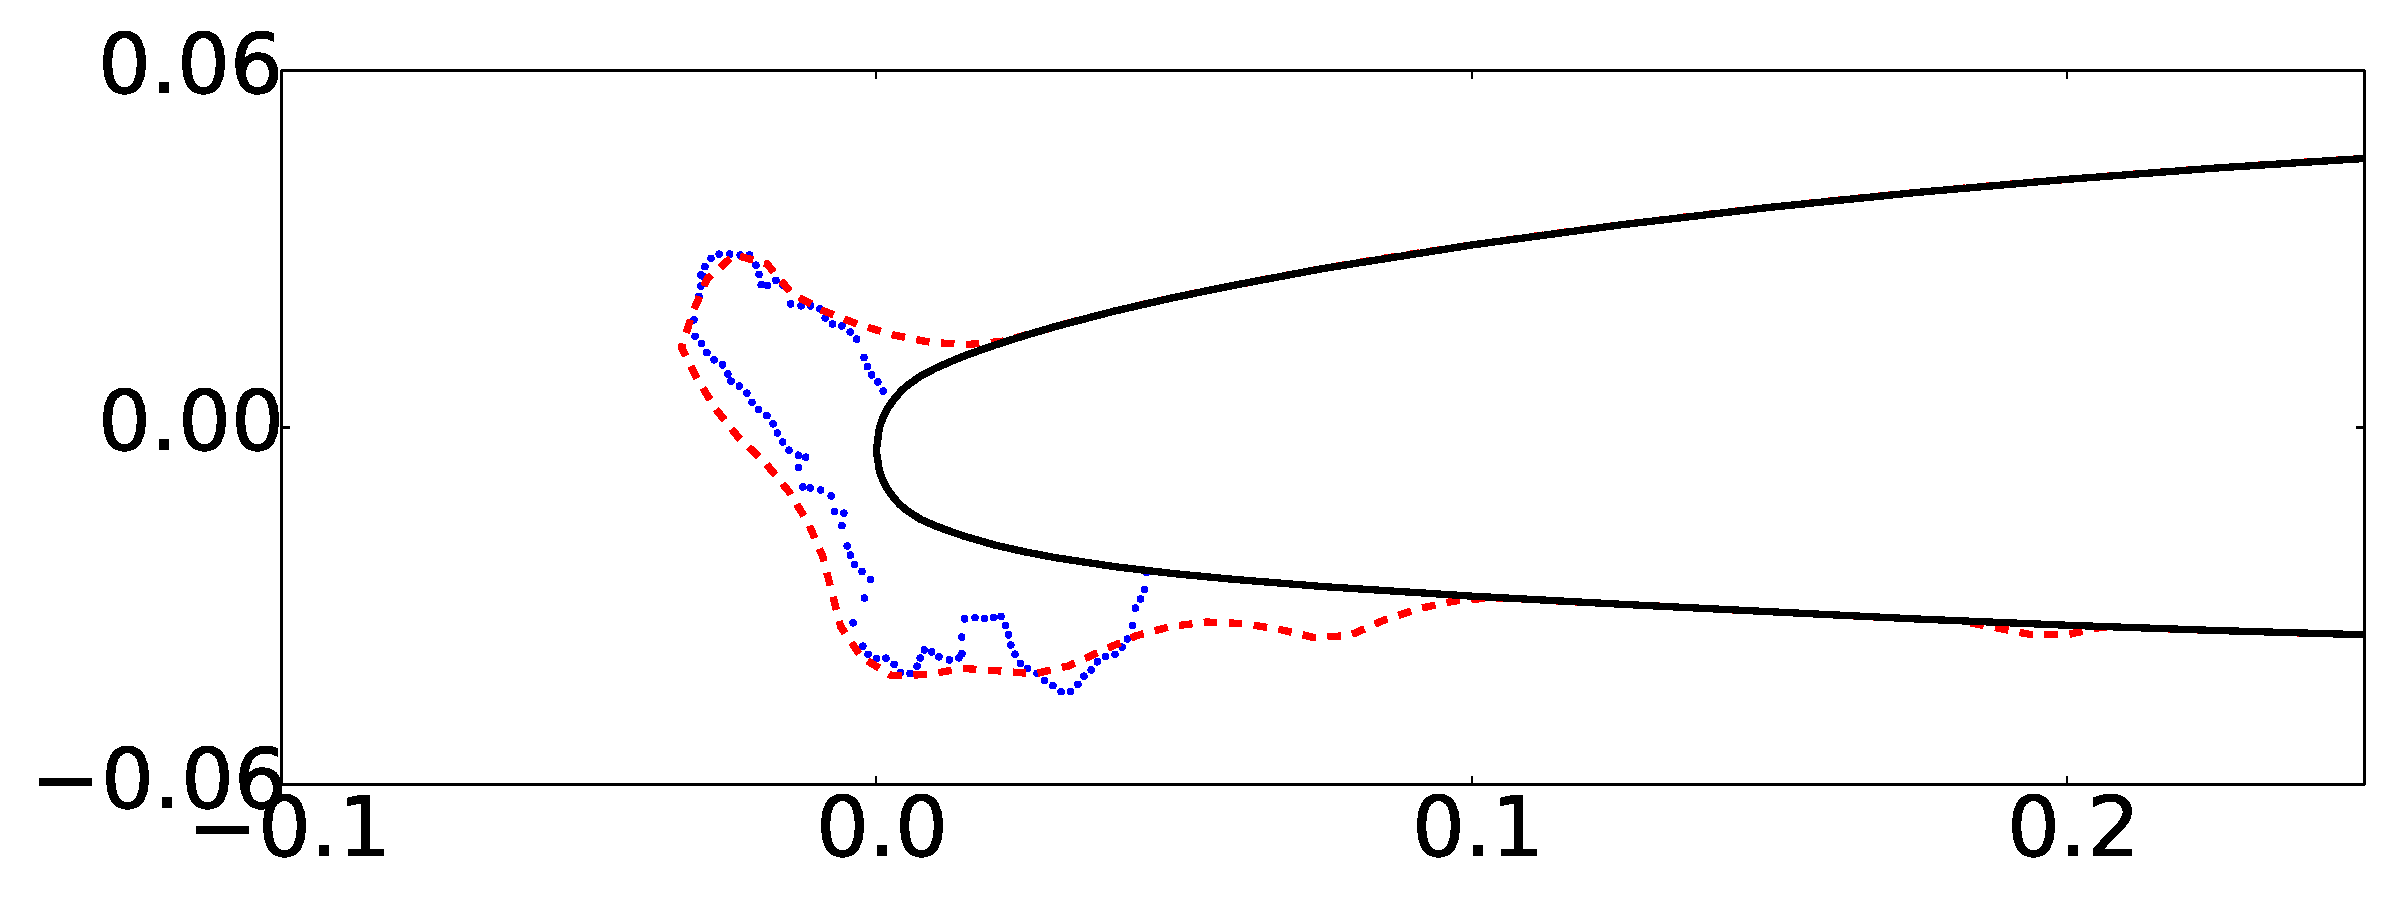
\includegraphics[width=1\textwidth]{ReconstructionE3} \\
    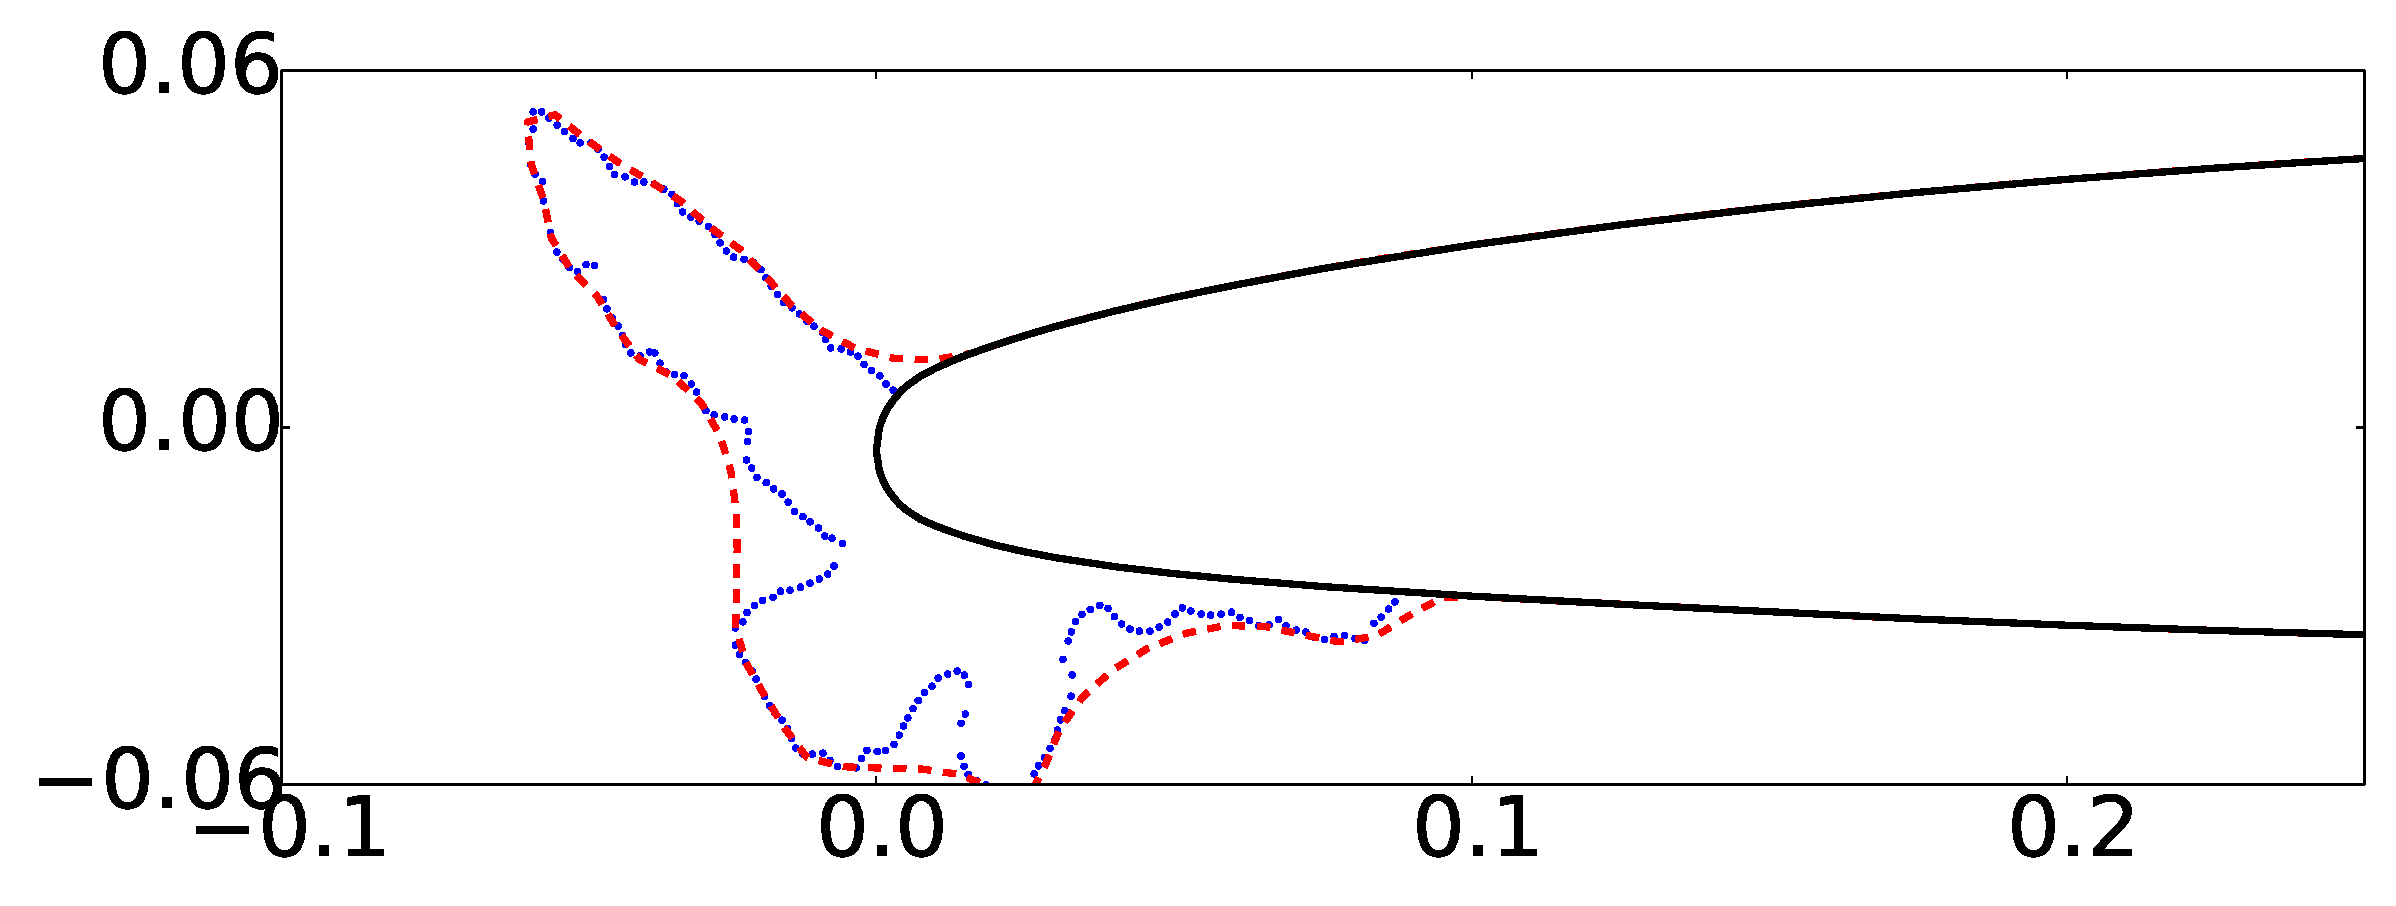
\includegraphics[width=1\textwidth]{ReconstructionE4} \\
\end{columns}
\begin{center}
{\bf Ice Reconstructions}
\end{center}
\end{frame}
\begin{frame}
\frametitle{Statistics: 3D Wing}
\label{sec-3-8}


\begin{columns}[c]
  \column{0.37\textwidth}
    \centering
    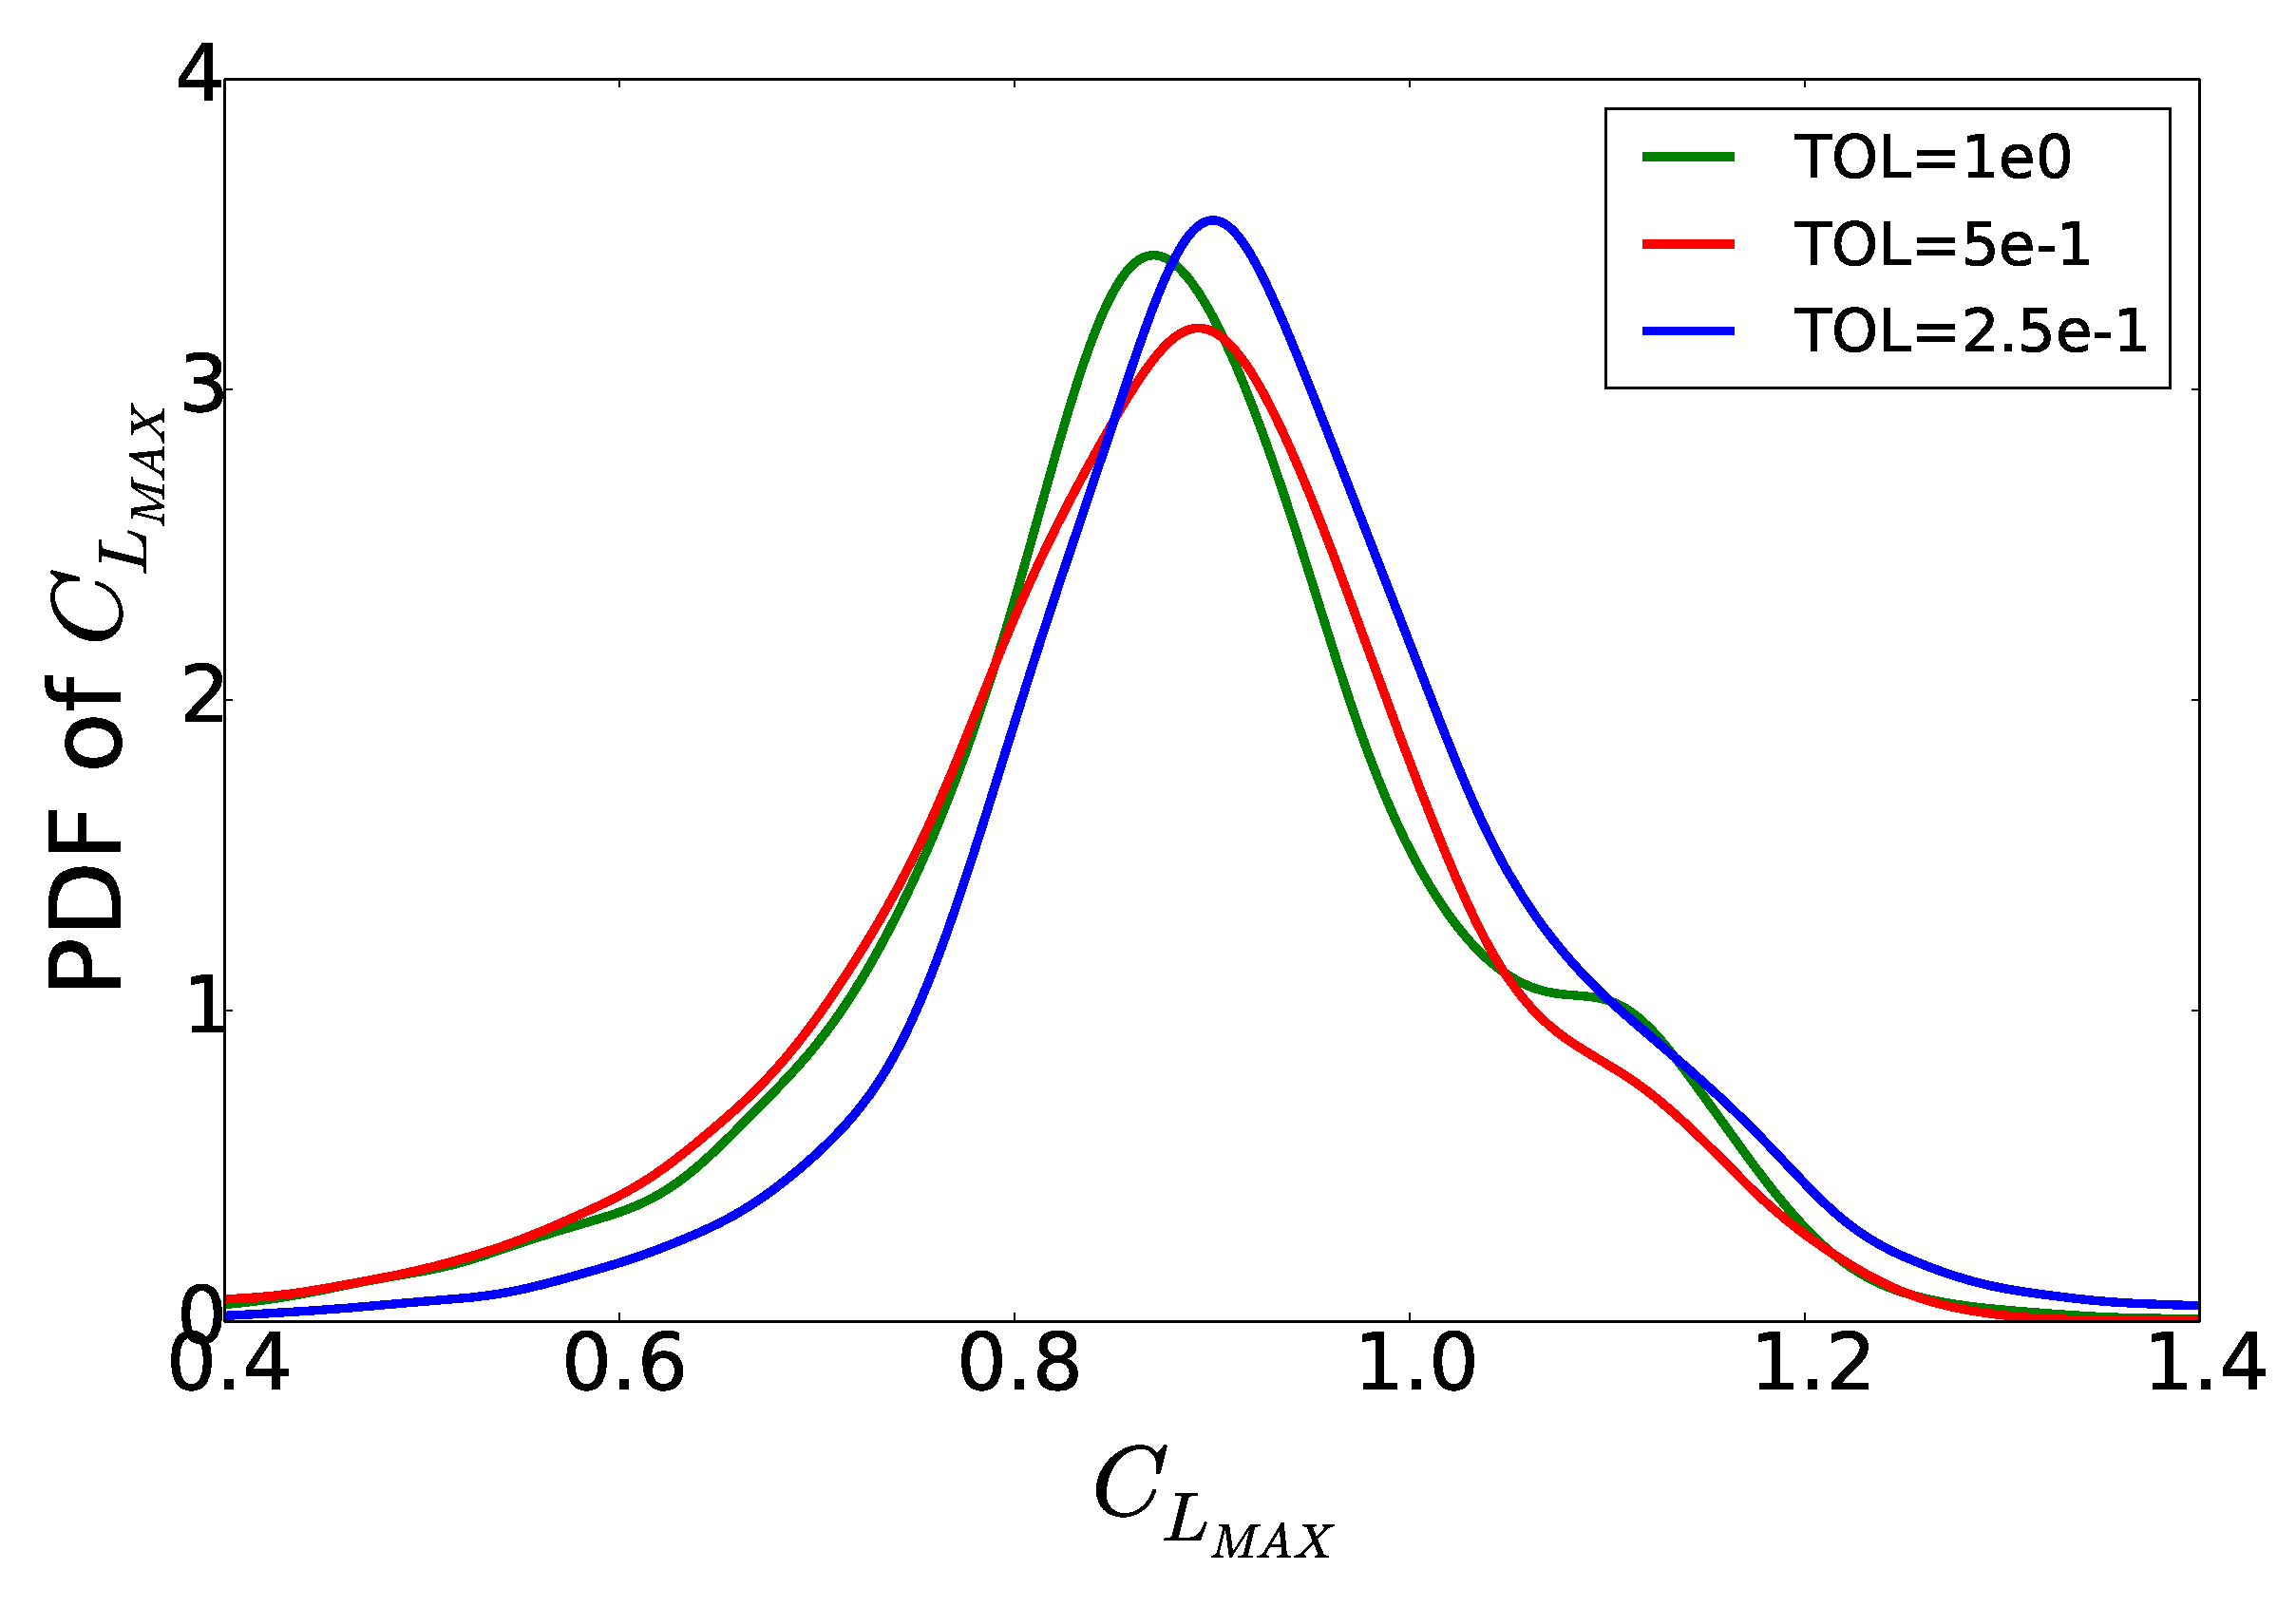
\includegraphics[width=1\textwidth]{PDFCLMAX} \\
    $\bm{C_L}$ {\bf Statistics}
  \column{0.37\textwidth}
    \centering
    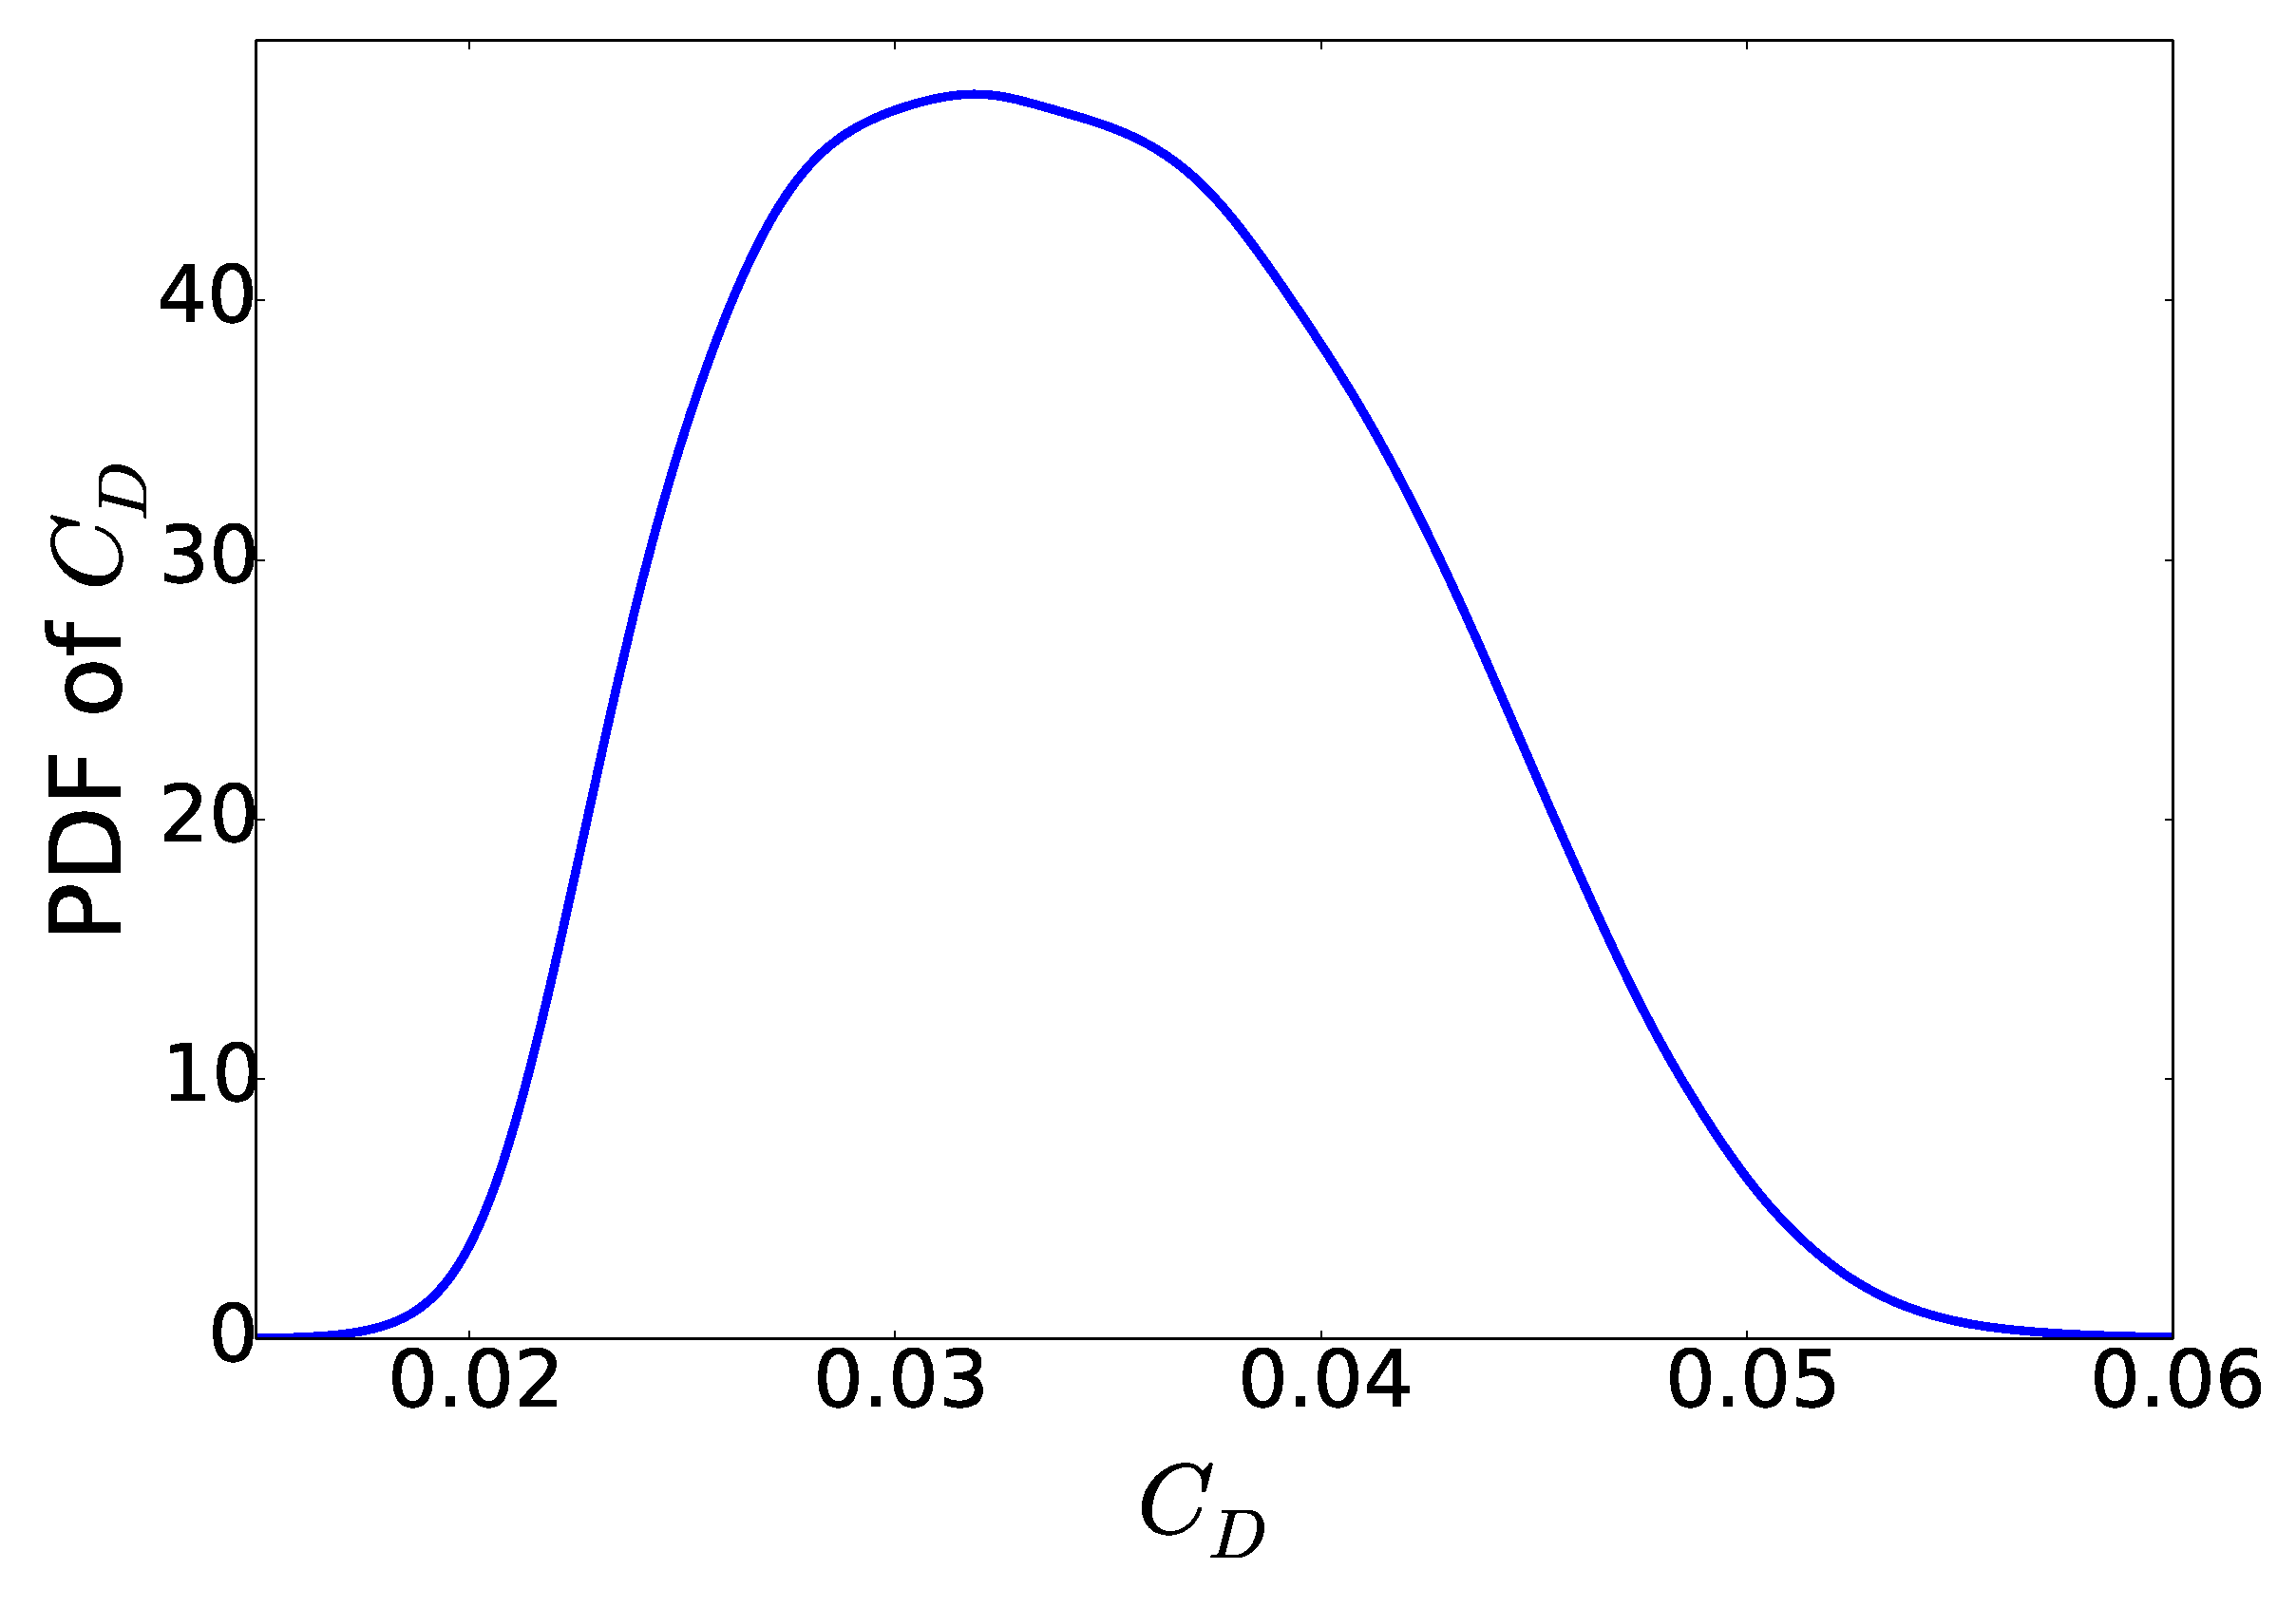
\includegraphics[width=1\textwidth]{PDFCDMAX} \\
    $\bm{C_D}$ {\bf Statistics}
\end{columns}



\begin{center}
\begin{tabular}{lrrrrr}
            &  Width  &  Position  &  Height  &  POD 1  &  POD 2  \\
\hline
 T ($C_L$)  &   0.03  &      0.69  &    0.15  &   0.11  &   0.14  \\
\end{tabular}
\end{center}



\begin{itemize}
\item Our surrogate is an explicit polynomial function of the input
  variables, making statistical inference easy/quick
\item PCE surrogate computed using 1,103 sparse grid points
\item Sobol index $T_i = \frac{\mathbb{E}\left[ Var\left(
  Y|Z_{-i}\right)\right]}{Var\left( Y\right)}$ is a measure of how much
  $Z_i$ contributes to the total variance of $Y(\bv{Z})$
\item For our parameter ranges, position perturbation accounts for most of
  the statistical variation
\end{itemize}
\end{frame}
\begin{frame}
\frametitle{Statistics: 3D Wing}
\label{sec-3-9}


\begin{itemize}
\item Analyze statistical clustering of horns that produce bottom and top
  $10\%$ of $C_L$ variation
\end{itemize}

\begin{columns}[c]
  \column{0.40\textwidth}
    \centering
    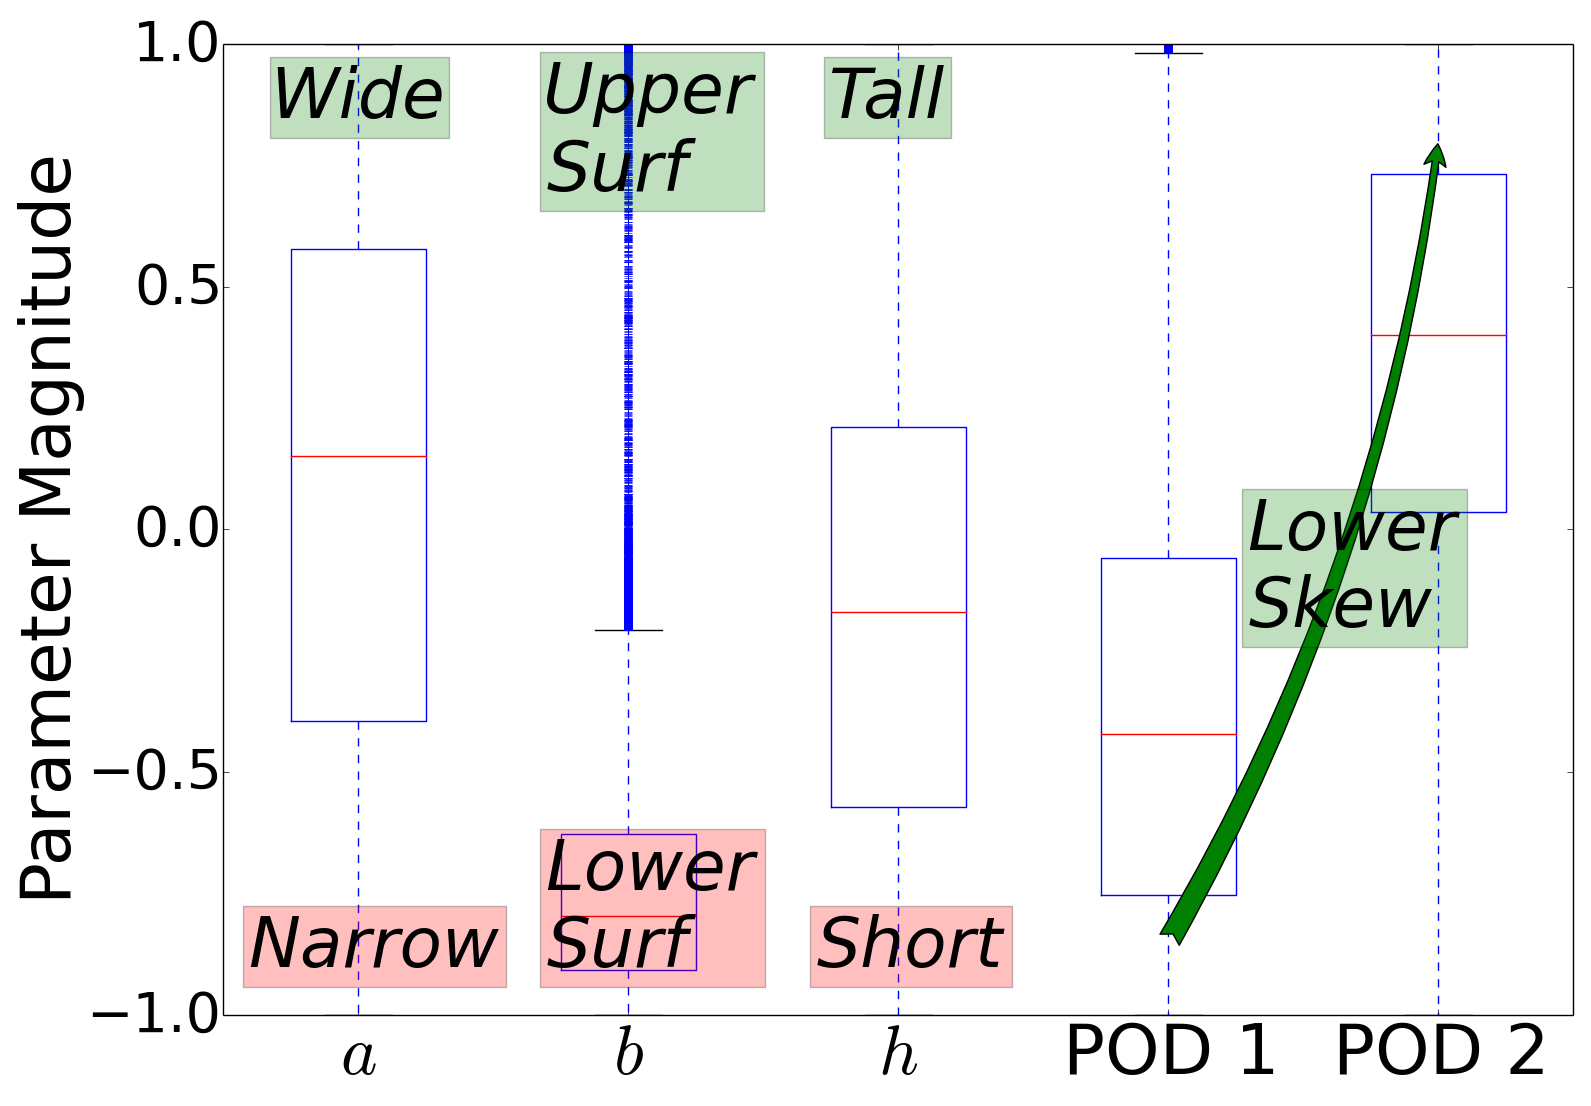
\includegraphics[width=1\textwidth]{GoodHornParamLocs.png} \\
    {\bf Favorable Horns}
    \begin{itemize}
      \item Wider/rounded
      \item Lower surface
      \item Shorter
      \item Gentle downward skew
    \end{itemize}
  \column{0.40\textwidth}
    \centering
    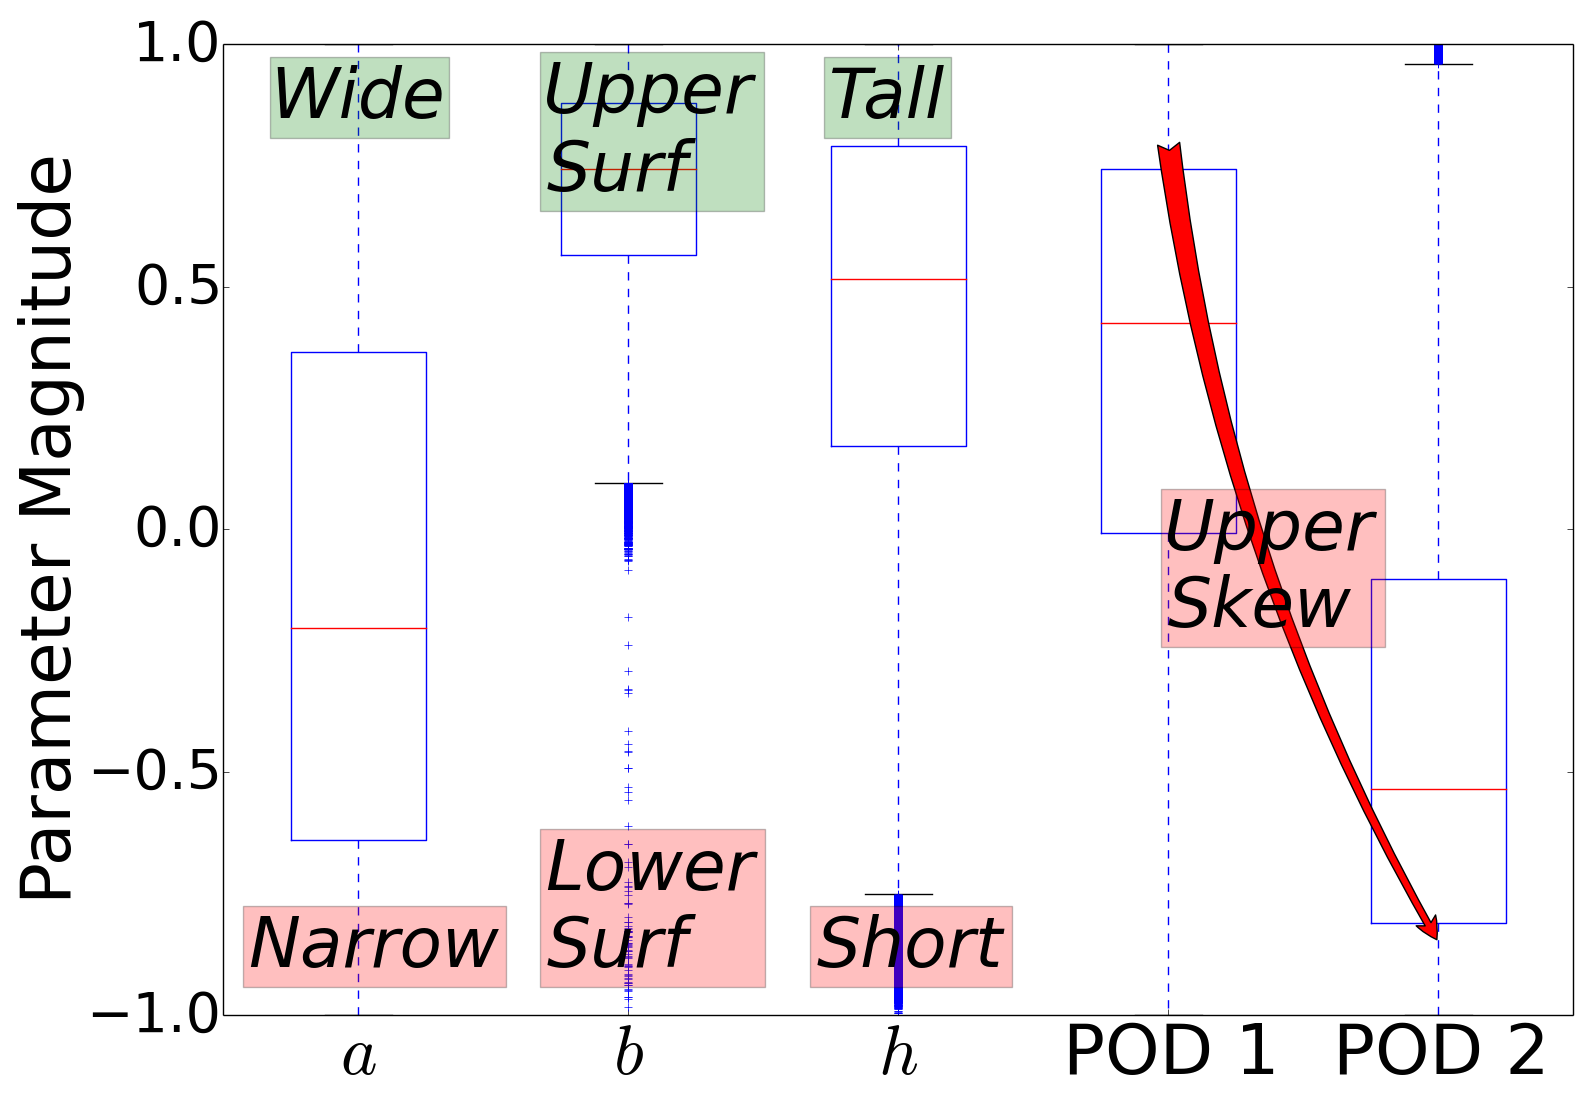
\includegraphics[width=1\textwidth]{BadHornParamLocs.png} \\
    {\bf Unfavorable Horns}
    \begin{itemize}
      \item Sharper/narrower
      \item Upper surface
      \item Taller
      \item Sharp, upper skew shape
    \end{itemize}
\end{columns}
\end{frame}
\begin{frame}
\frametitle{Flow Solutions}
\label{sec-3-10}


\begin{columns}[c]
  \column{0.30\textwidth}
    \centering
    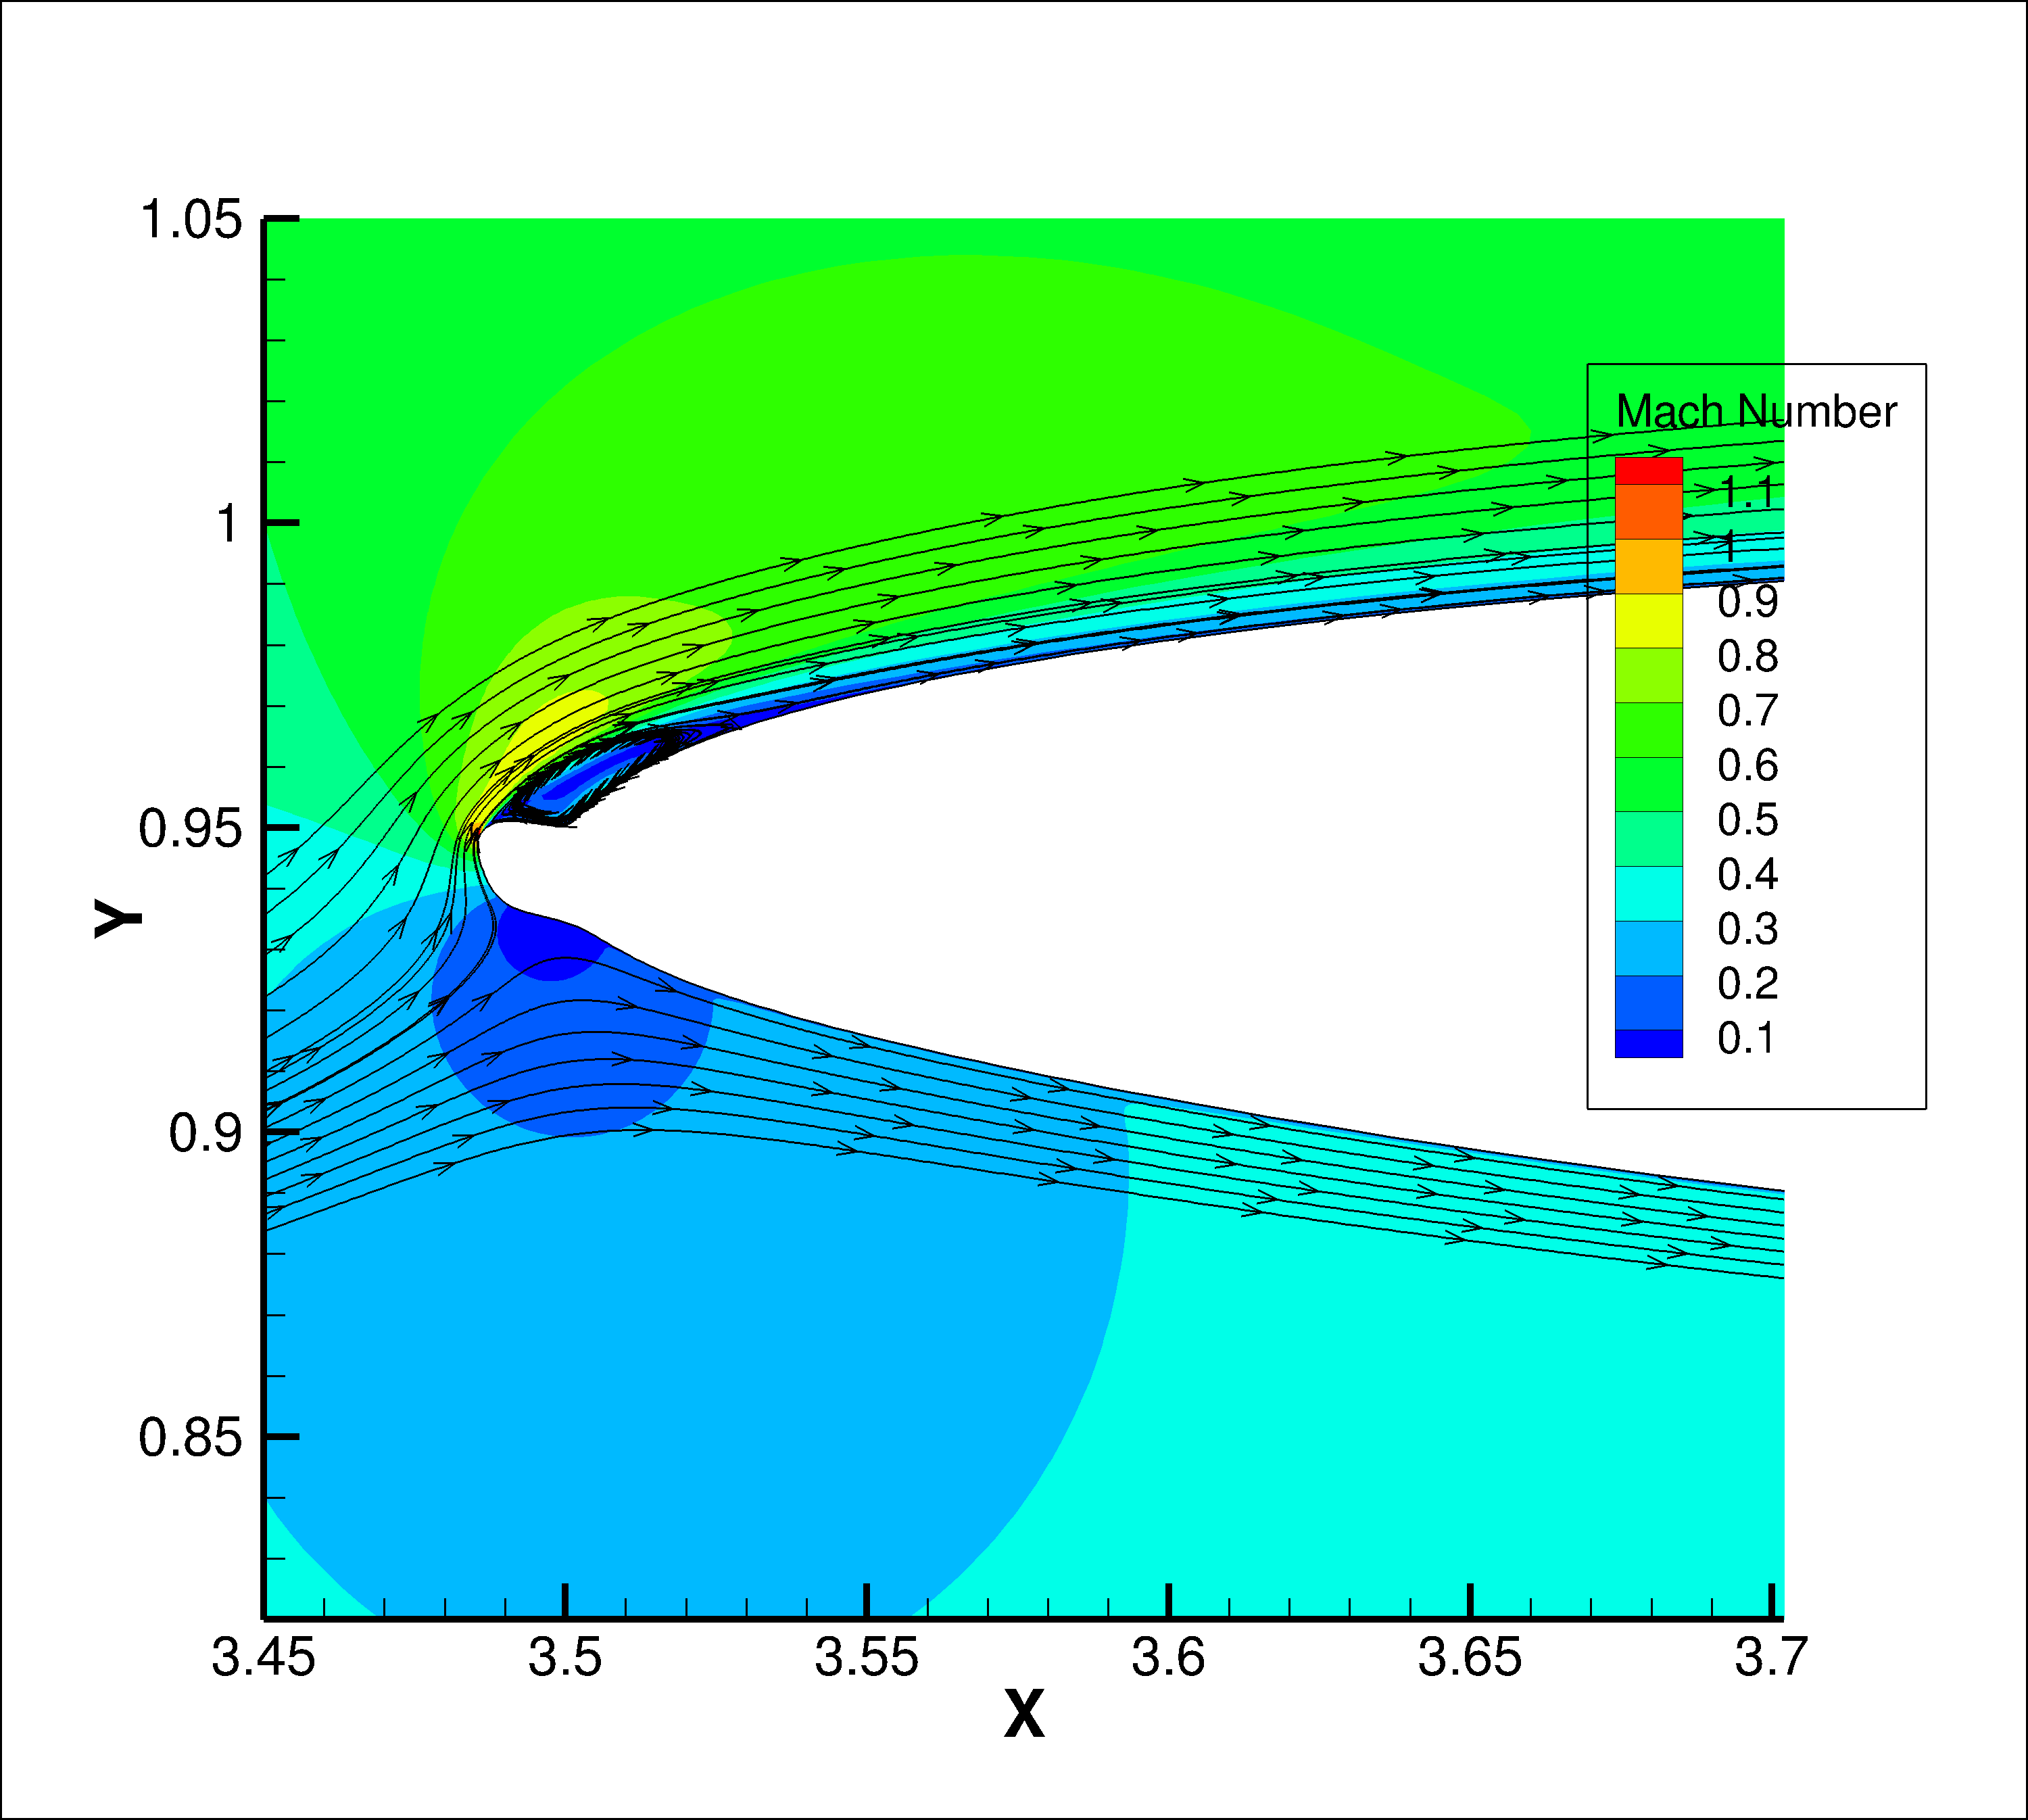
\includegraphics[width=1\textwidth]{GoodHorn.png} \\
    {\bf Favorable Position}
    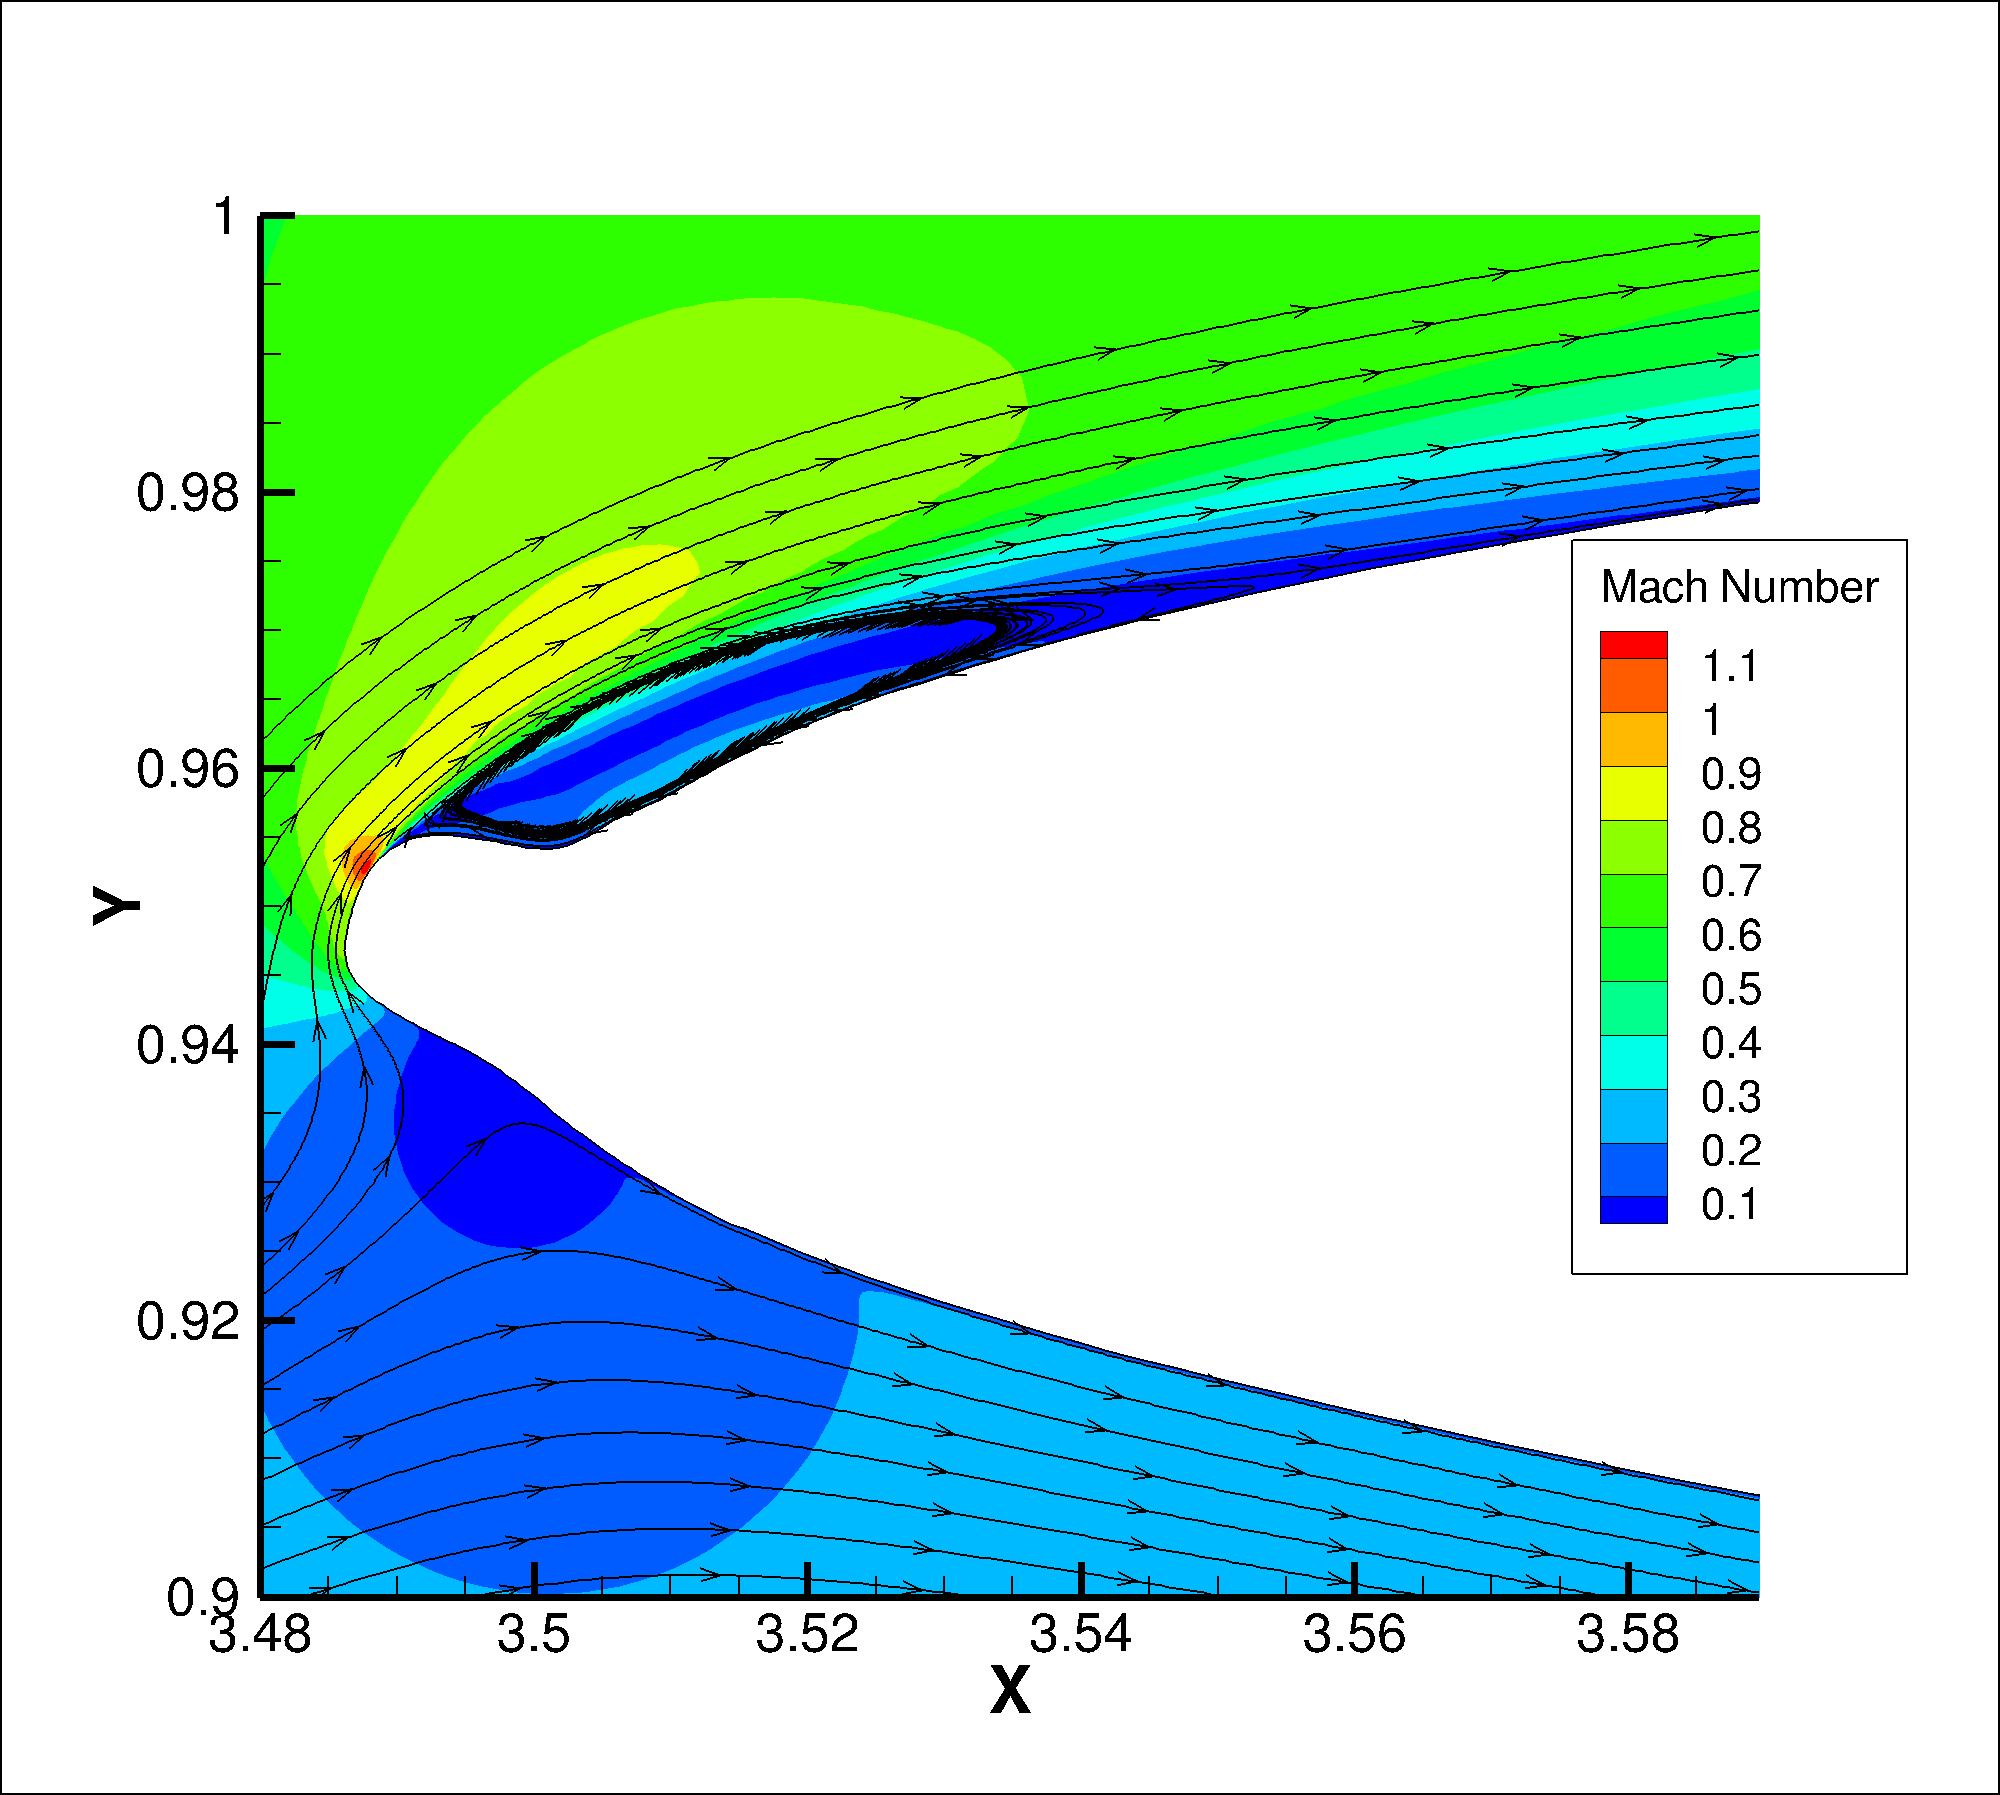
\includegraphics[width=1\textwidth]{GoodHornPOD.png} \\
    {\bf Favorable shape skew}
  \column{0.30\textwidth}
    \centering
    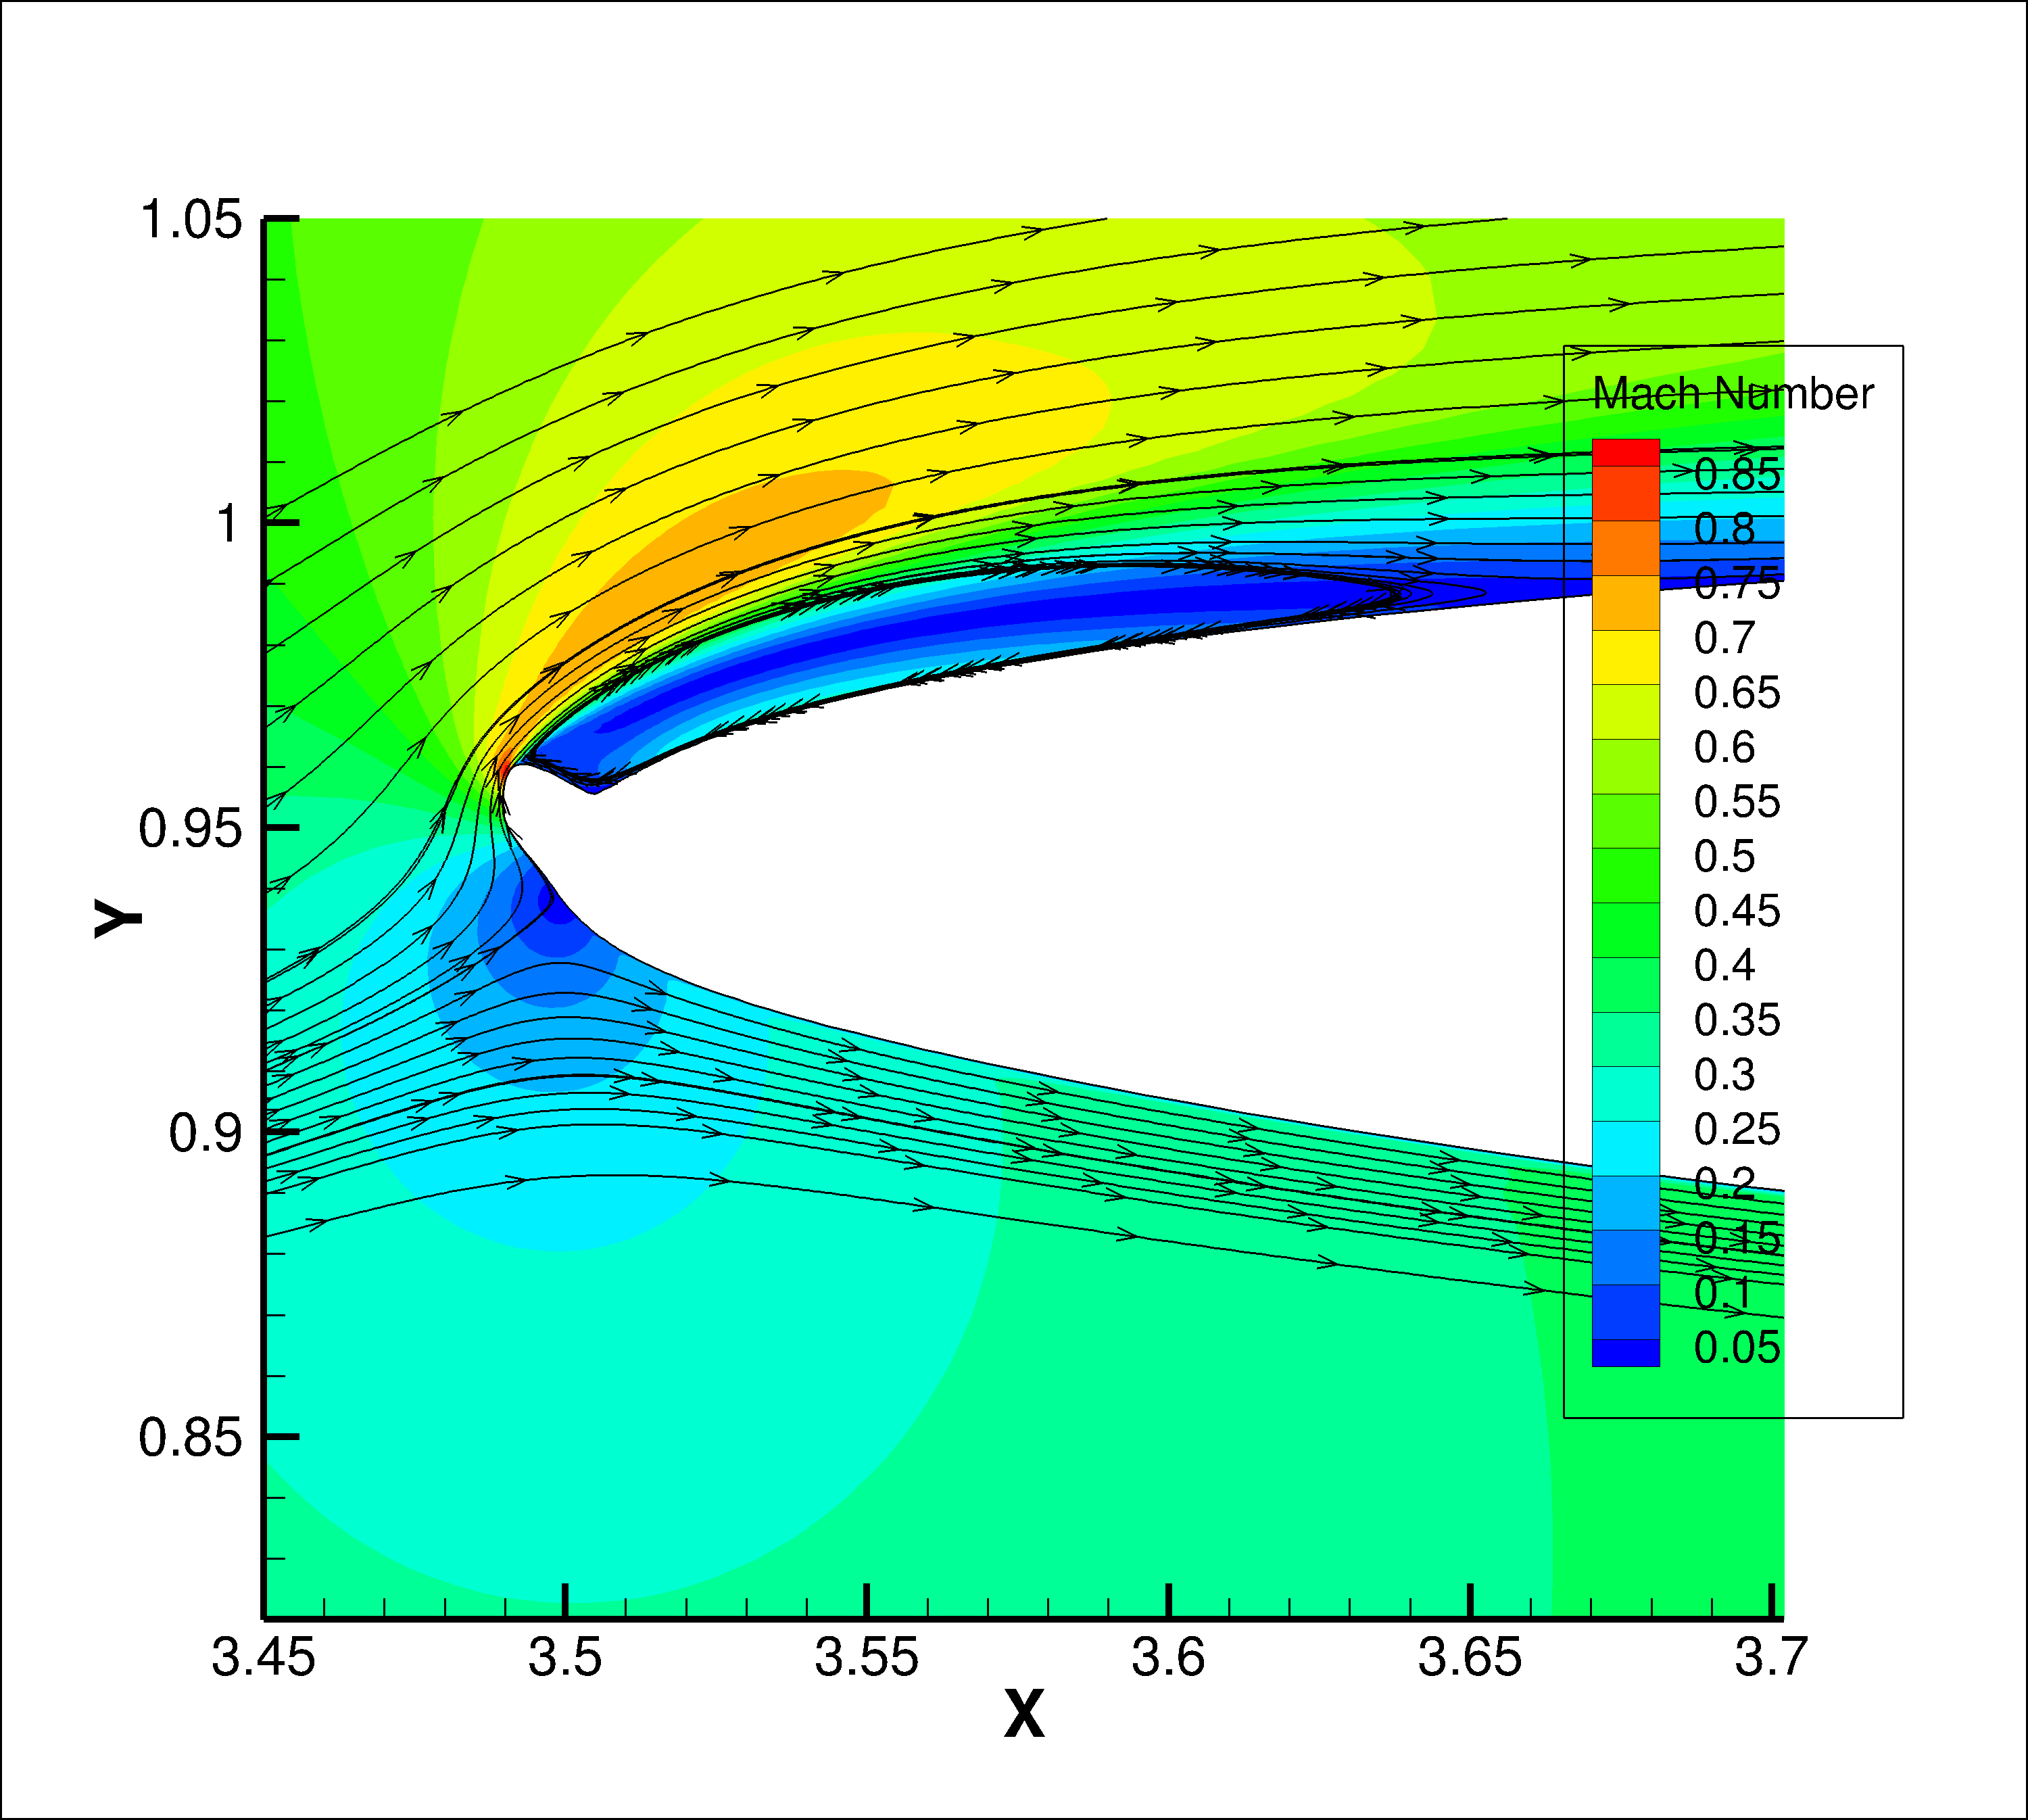
\includegraphics[width=1\textwidth]{BadHorn.png} \\
    {\bf Unfavorable Position}
    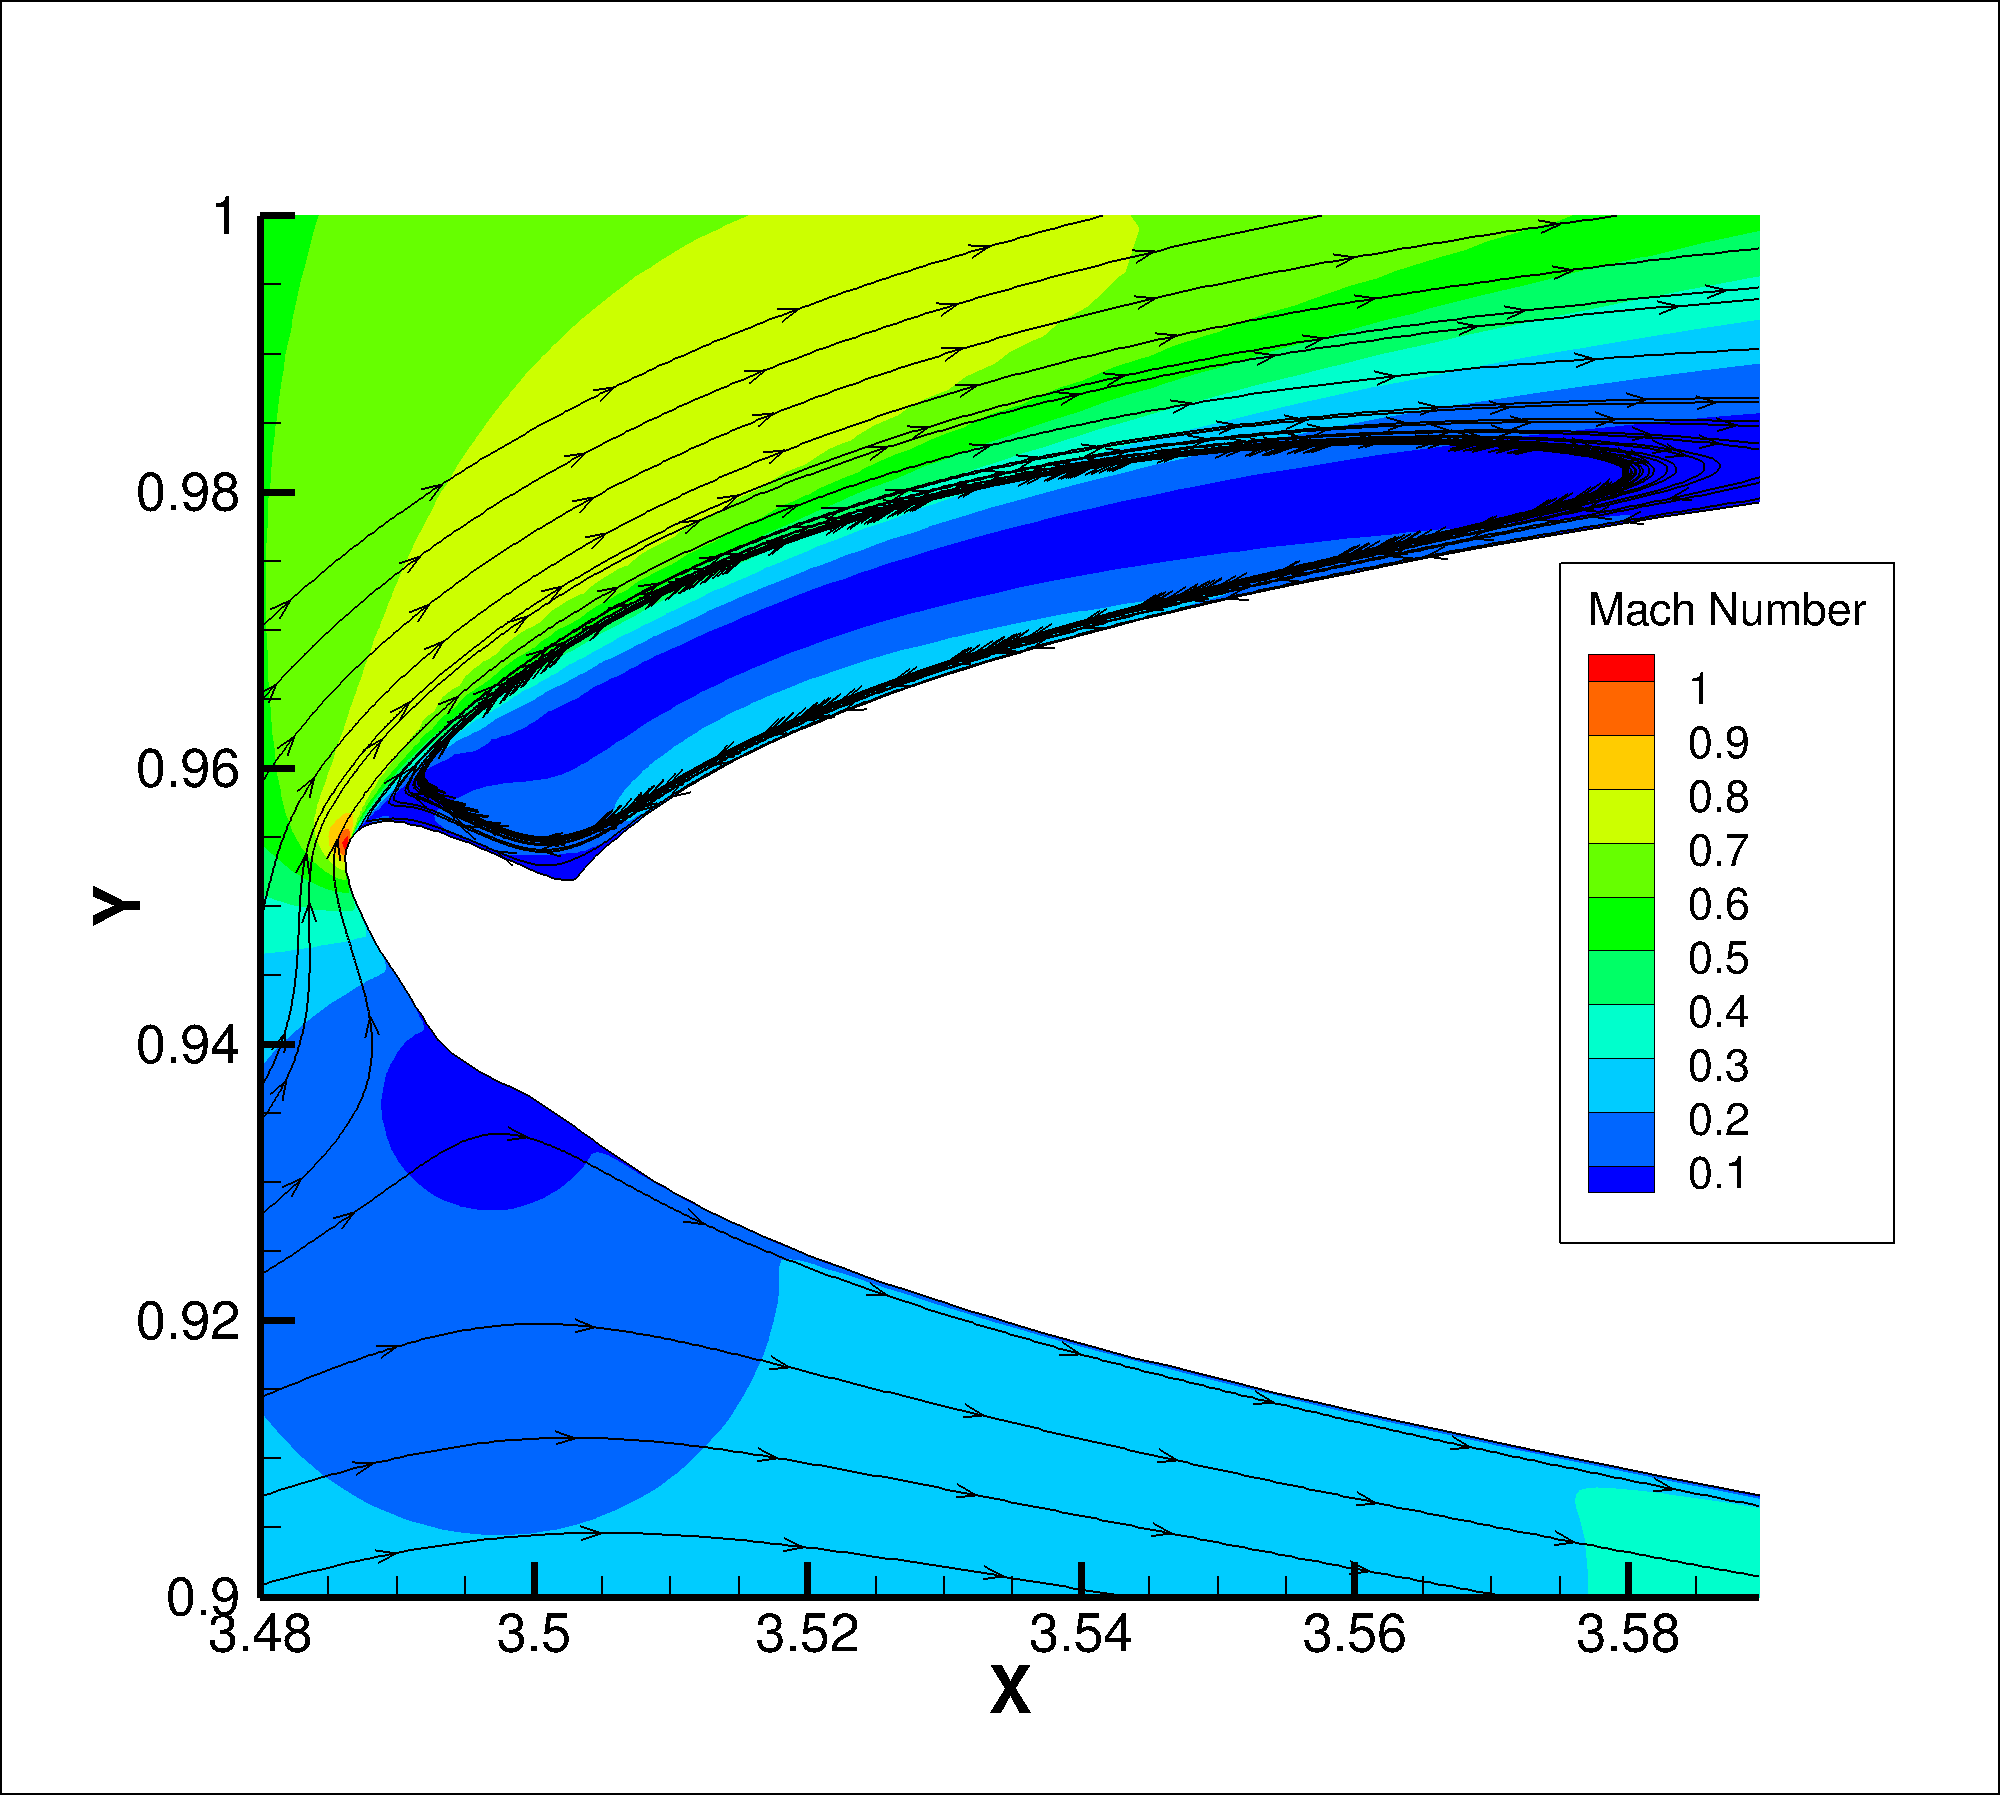
\includegraphics[width=1\textwidth]{BadHornPOD.png} \\
    {\bf Unfavorable shape skew}
\end{columns}
\end{frame}
\section{Icing: Computational-Based UQ}
\label{sec-4}
\begin{frame}
\frametitle{Motivation}
\label{sec-4-1}

\begin{itemize}
\item \textbf{Investigate uncertainty in the physical process of icing}
\begin{itemize}
\item What is the statistical effect of uncertainty in physical parameters?
\begin{itemize}
\item Free-stream temperature
\item Angle of attack
\item Convective heat transfer
\item Droplet diameter distribution
\item Accretion time
\end{itemize}
\end{itemize}
\end{itemize}
\end{frame}
\begin{frame}
\frametitle{Airfoil Icing Code Flowchart}
\label{sec-4-2}

\fontsize{7}\selectfont
% Define the layers to draw the diagram
\pgfdeclarelayer{background}
\pgfdeclarelayer{foreground}
\pgfsetlayers{background,main,foreground}

% Define block styles used later

\tikzstyle{sensor}=[draw, fill=blue!20, text width=5em, 
    text centered, minimum height=2.5em,drop shadow]
\tikzstyle{ann} = [above, text width=5em, text centered]
\tikzstyle{wa} = [sensor, text width=7.5em, fill=blue!20, 
    minimum height=3em, rounded corners, drop shadow]

% Define distances for bordering
\def\blockdist{2.3}
\def\edgedist{2.5}

\begin{tikzpicture}
    \node (CleanAirfoil) [wa]  {Clean Airfoil Geometry};
    \path (CleanAirfoil)+(4,2.5) node (FlowSolver) [wa] {Mesh/Flow Solver};
    \path (FlowSolver)+(0,-1.25) node (Droplet) [wa] {Droplet\\Advection Module};
    \path (Droplet)+(0,-1.25) node (ThermoModule) [wa] {Thermodynamic Module};
    \path (ThermoModule)+(0,-1.25) node (IcedAirfoil) [wa] {Iced Airfoil Geometry};
    \path (CleanAirfoil)+(8,0) node (FinalAirfoil) [wa] {Final Iced Airfoil Geometry};

    \path [draw, ->, thick] (CleanAirfoil.north) |- node [above] {} (FlowSolver.west);
    \path [draw, ->, thick] (FlowSolver.south) -- node [below] {} (Droplet.north);
    \path [draw, ->, thick] (Droplet.south) -- node [below] {} (ThermoModule.north);
    \path [draw, ->, thick] (ThermoModule.south) -- node [below] {} (IcedAirfoil.north);
    \path [draw, ->, thick] (IcedAirfoil.east) -| node [above] {} (FinalAirfoil.south);
    \path [draw, ->, thick] (IcedAirfoil.east) -- ++(0.75,0cm) |- node [above]
                      {} (FlowSolver.east);

    \begin{pgfonlayer}{background}
        \path (FlowSolver.west)+(-1,1) node (a) {};
        \path (IcedAirfoil.east)+(1,-1) node (b) {};
        \path[fill=orange!20,rounded corners, draw=black!50, dashed] (a) rectangle (b);
            
    \end{pgfonlayer}

\end{tikzpicture}
\end{frame}
\begin{frame}
\frametitle{Droplet Advection}
\label{sec-4-3}

\begin{equation*}
  \begin{align}
    \frac{d \bv{x}}{d t} &= \bv{v} \\
    m \frac{d \bv{v}}{d t} &= \frac{1}{2} \rho_g C_D \pi r^2 ||\bv{v_g} - \bv{v}|| (\bv{v_g} - \bv{v}) + m \bv{g}
  \end{align}
\end{equation}

\begin{columns}[c]
  \column{0.5\textwidth}
    \centering
    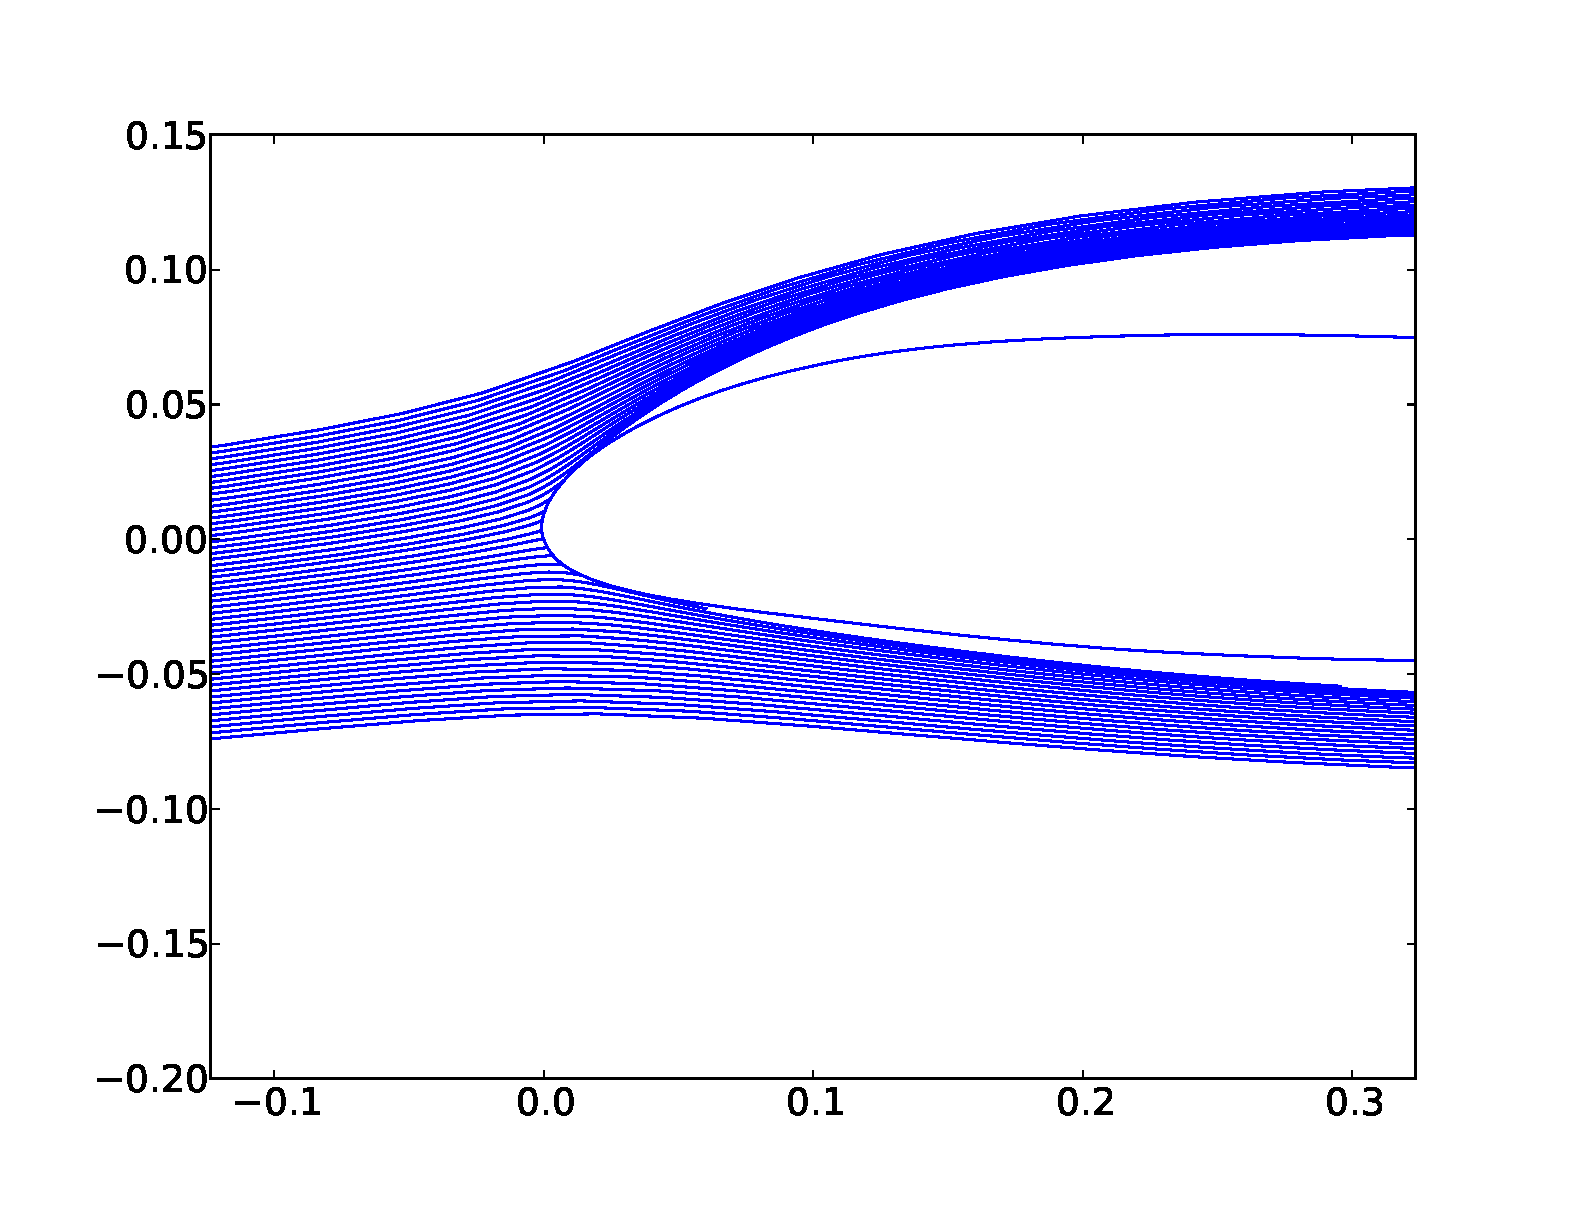
\includegraphics[width=1\textwidth]{ExampleR10em6} \\
    {\bf R = 10$\mu$m}
  \column{0.5\textwidth}
    \centering
    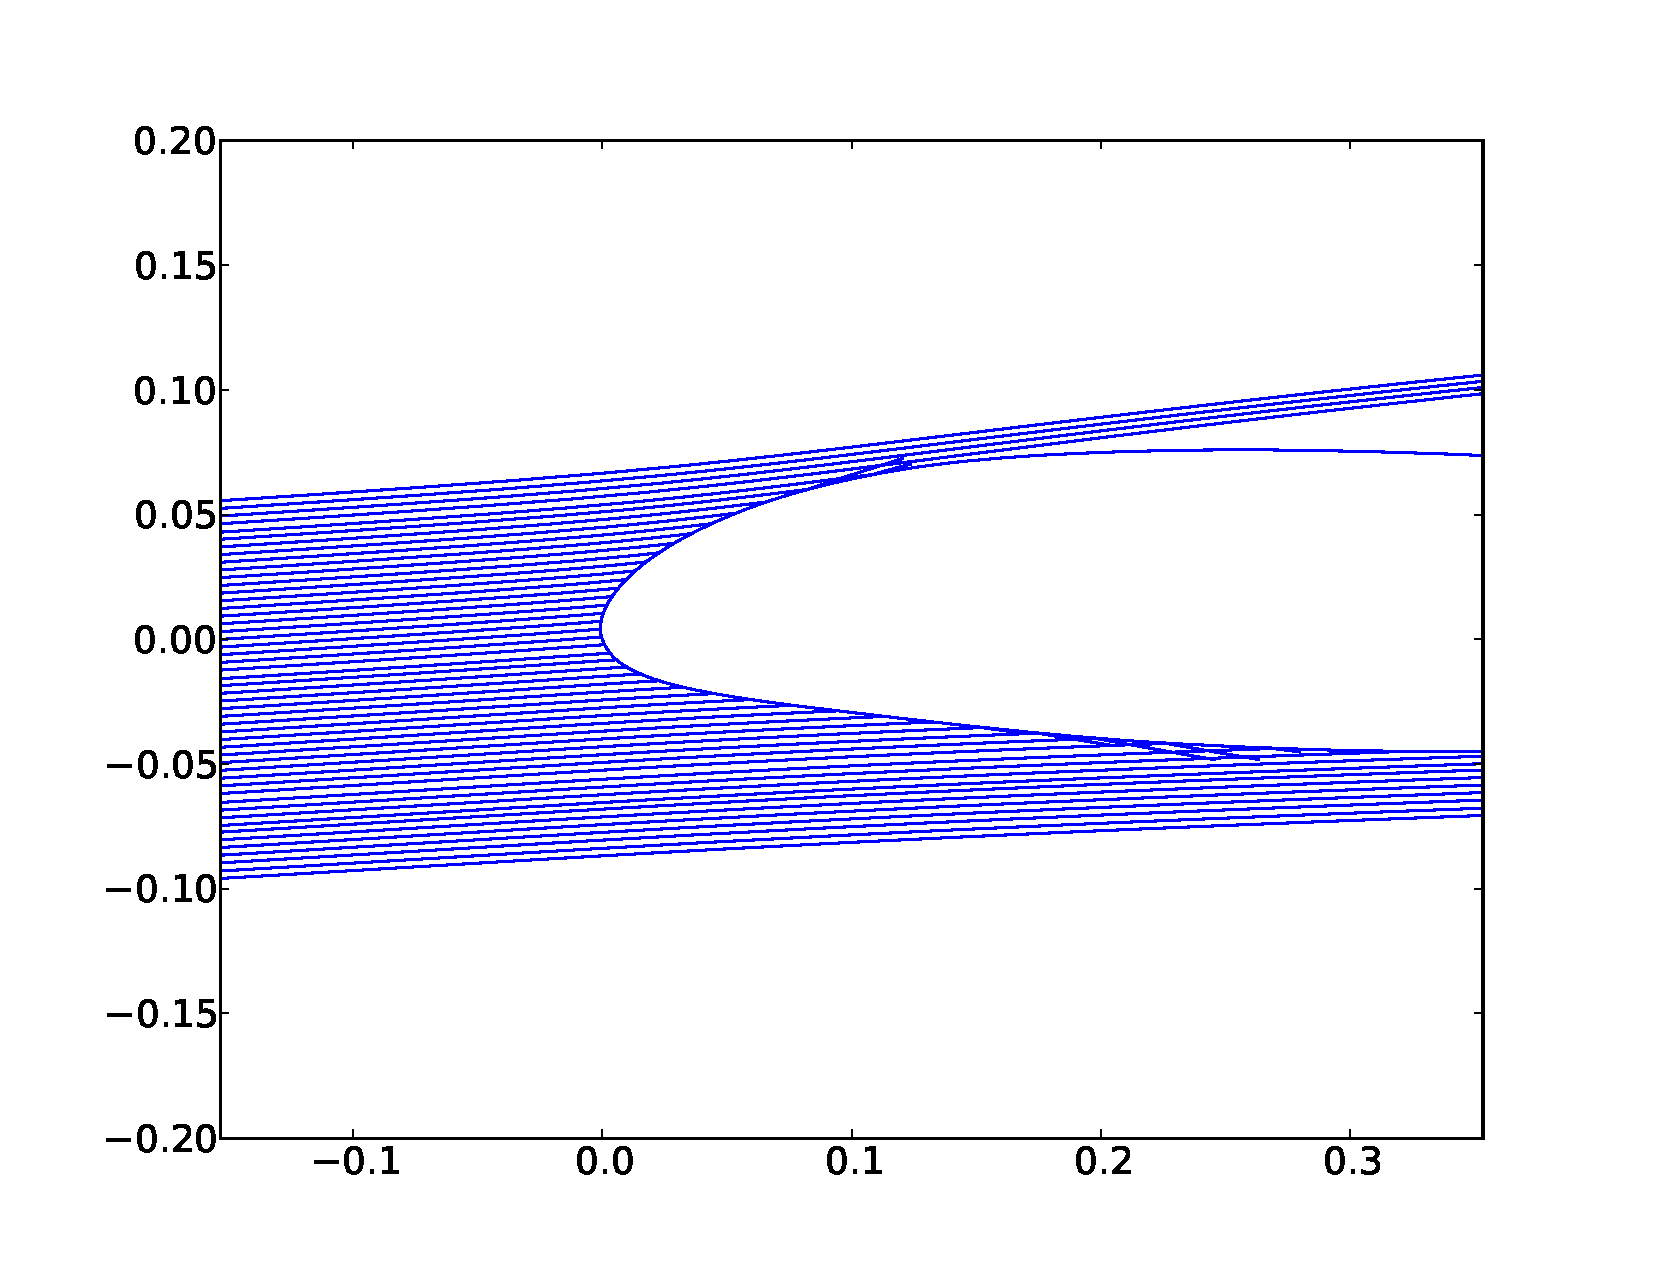
\includegraphics[width=1\textwidth]{ExampleR100em6} \\
    {\bf R = 100$\mu$m}
\end{columns}
\end{frame}
\begin{frame}
\frametitle{Thermodynamics}
\label{sec-4-4}

\begin{equation*}
  \begin{align}
    \rho_w \left \lbrace \frac{\partial h_f}{\partial t} + \nabla \cdot (\bv{u_f} h_f) \right \rbrace &= \dot{m}_{imp} - \dot{m}_{ice} \\
    \rho_w \left \lbrace \frac{\partial (h_f c_W T)}{\partial t} + \nabla \cdot (\bv{u_f} h_f c_W T) \right \rbrace &= \left [ c_W T_d + \frac{u_d^2}{2} \right ] \dot{m}_{imp} \\
    & +(L_{fus} - c_{ice}T)\dot{m}_{ice} \\
    & + c_H (T_{\infty} - T)
  \end{align}
\end{equation}

\begin{itemize}
\item \textbf{Mass}
\begin{itemize}
\item Enters through impinging droplets
\item Exits via evaporation/sublimation and freezing
\end{itemize}
\item \textbf{Energy}
\begin{itemize}
\item Enters through impinging droplets, freezing of ice
\item Exits via evaporation/sublimation, radiation, convection
\end{itemize}
\item Solved explicitly using finite volume discretization with Roe scheme upwinding
\end{itemize}
\end{frame}
\begin{frame}
\frametitle{Preliminary Intermediate Results: Ice Shapes}
\label{sec-4-5}

    \centering
    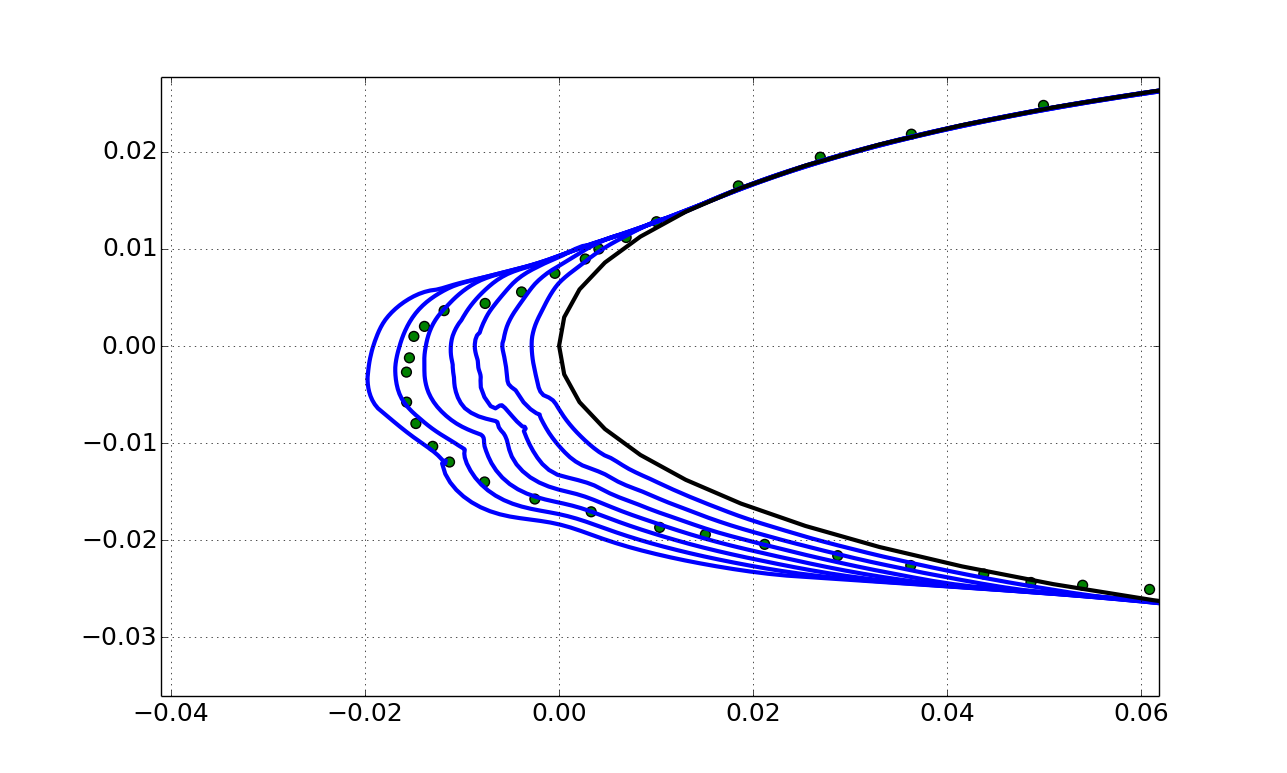
\includegraphics[width=0.65\textwidth]{Rime405Example.png}

\begin{itemize}
\item NACA0012, $\alpha = 4^o$, $T_{\infty} = 256 K$, $U_{\infty}$ = 103 m/s, MVD = 20 $\mu m$, LWC = 0.55 g/m$^3$, Re = 4.14 million, $\Delta T$ = 7 min
\item Low temperatures: convective heat transfer high enough to freeze all incoming droplets instantly (rime)
\end{itemize}
\end{frame}
\begin{frame}
\frametitle{Work In-Progress}
\label{sec-4-6}

\begin{itemize}
\item Implement rough-wall extension in Spalart-Almaras turbulence model
\item Implement neglected mass/energy transfer mechanisms
\item Verify icing calculations against published results
\item Perform UQ studies, investigate sensitivity to physical parameters
\begin{itemize}
\item Temperature, convective heat transfer coefficient, Reynolds number, MVD, LWC, angle of attack, etc.
\end{itemize}
\end{itemize}
\end{frame}
\section{Fires: Introduction}
\label{sec-5}
\begin{frame}
\frametitle{Motivation}
\label{sec-5-1}

\begin{itemize}
\item \textbf{Cargo hold fires are a significant safety hazard}
\begin{itemize}
\item Tight constraints for detection/suppression
\item FAA requires detection of cargo fire within 60 seconds of ignition\footnote{Blake, D. et. al. 2014 Fire Safety Highlights. Federal
Aviation Administration. Research Summary, 2014.
 }\textsuperscript{,}\,\footnote{Oztekin, E. S. Heat and mass transfer due to a small-fire in
an aircraft cargo compartment. \International Journal of Heat and Mass
Transfer\, Vol. 73, 2014, pp. 562-573.
 }
\end{itemize}
\end{itemize}
\centering
\begin{minipage}[b]{0.45\linewidth}
\begin{figure}[ht]
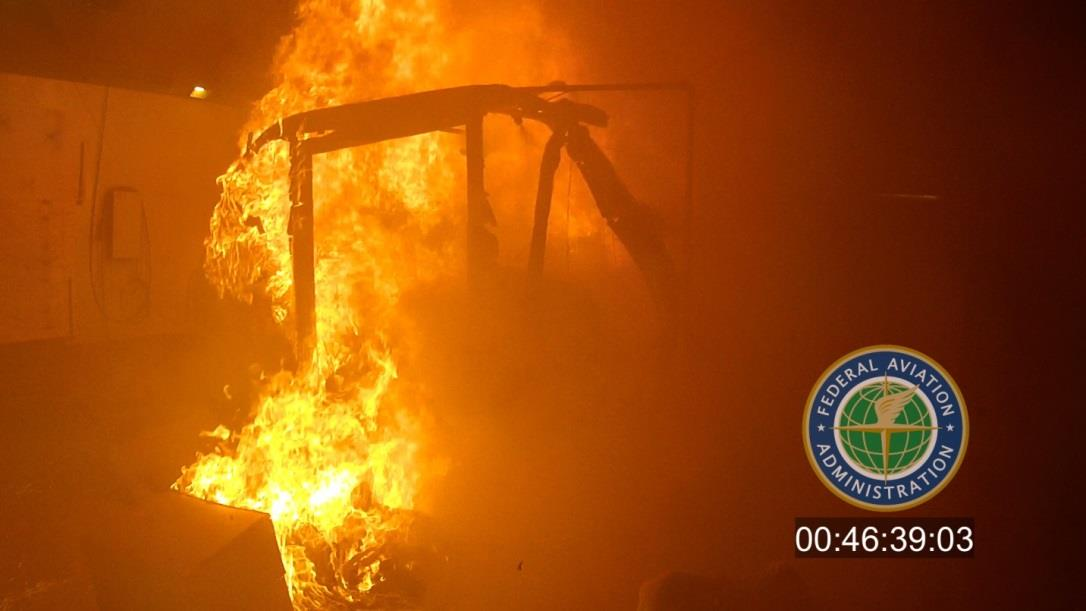
\includegraphics[width=0.9\textwidth]{CargoHoldFire1.png} \\
\textbf{Cargo hold fire generated from lithium-ion battery}
\end{figure}
\end{minipage}
\begin{minipage}[b]{0.45\linewidth}
\begin{figure}[ht]
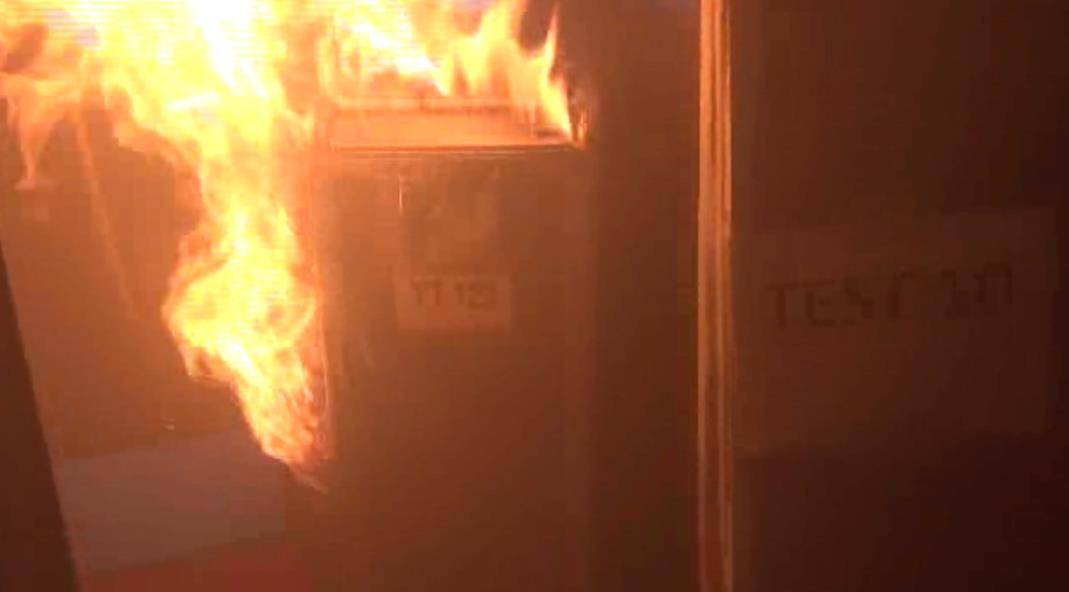
\includegraphics[width=0.9\textwidth]{CargoHoldFire2.png} \\
\textbf{Cargo hold fire generated from e-tablet}
\end{figure}
\end{minipage}
\end{frame}
\begin{frame}
\frametitle{Motivation}
\label{sec-5-2}

\begin{itemize}
\item \textbf{Current detection systems are overly conservative}\footnote{Blake. Aircraft cargo compartment smoke detector alarm incidents on U.S.-registered aircraft. \emph{FAA technical note} FAA-TN00/29, 2000.
 }
\begin{itemize}
\item 200-to-1 false alarm ratio (1995-99)
\item Unscheduled landings are expensive
\end{itemize}
\end{itemize}
\centering
\begin{minipage}[b]{0.45\linewidth}
\begin{figure}
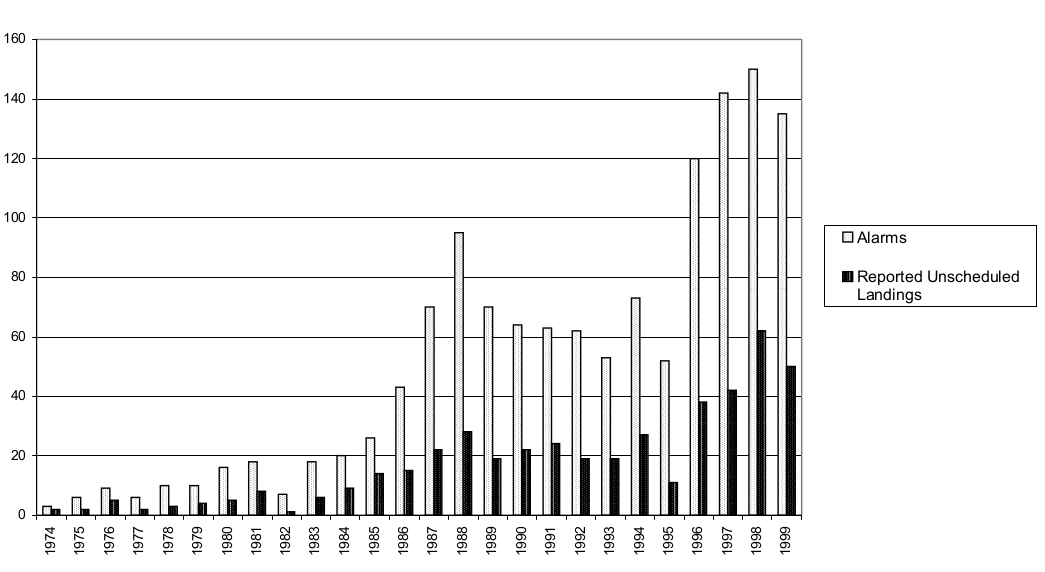
\includegraphics[width=0.9\linewidth]{alarmlandings.png} \\
\textbf{Alarms and Unscheduled Landings}
\end{figure}
\end{minipage}
\begin{minipage}[b]{0.45\linewidth}
\begin{figure}
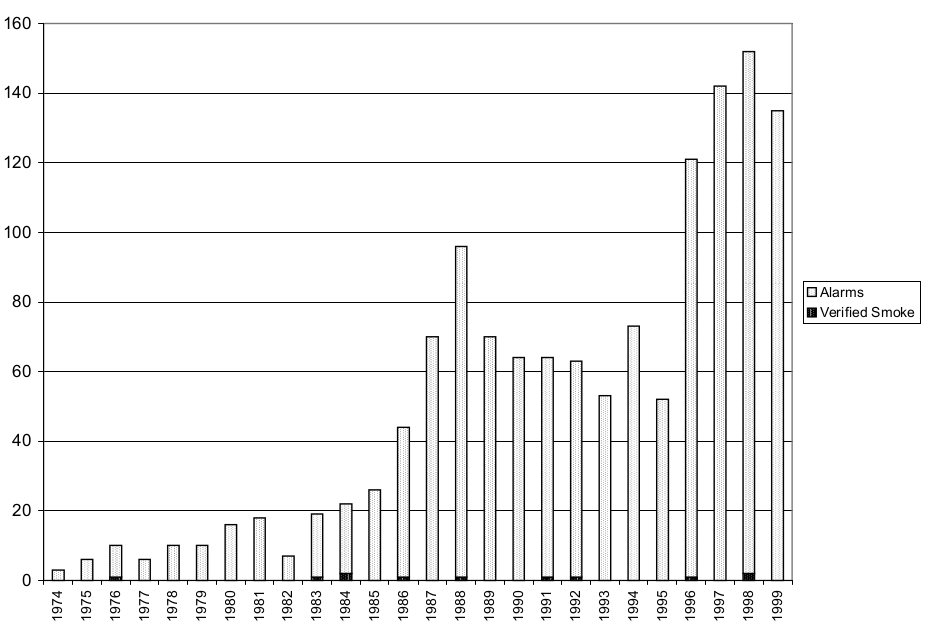
\includegraphics[width=0.9\linewidth]{alarms_vs_verified.png} \\
\textbf{False/Verified Alarms}
\end{figure}
\end{minipage}
\end{frame}
\begin{frame}
\frametitle{Motivation}
\label{sec-5-3}

\begin{itemize}
\item \textbf{Fire dynamics are sensitive to boundary condition uncertainty}
\begin{itemize}
\item Fire source location and temperature within cargo hold can vary
\item Cargo hold is cluttered with baggage, packages, pipes, etc.
\item Spatio-temporal fire plume development is affected by this uncertainty
\end{itemize}
\end{itemize}

\begin{minipage}[b]{0.45\linewidth}
\centering
\begin{figure}[ht]
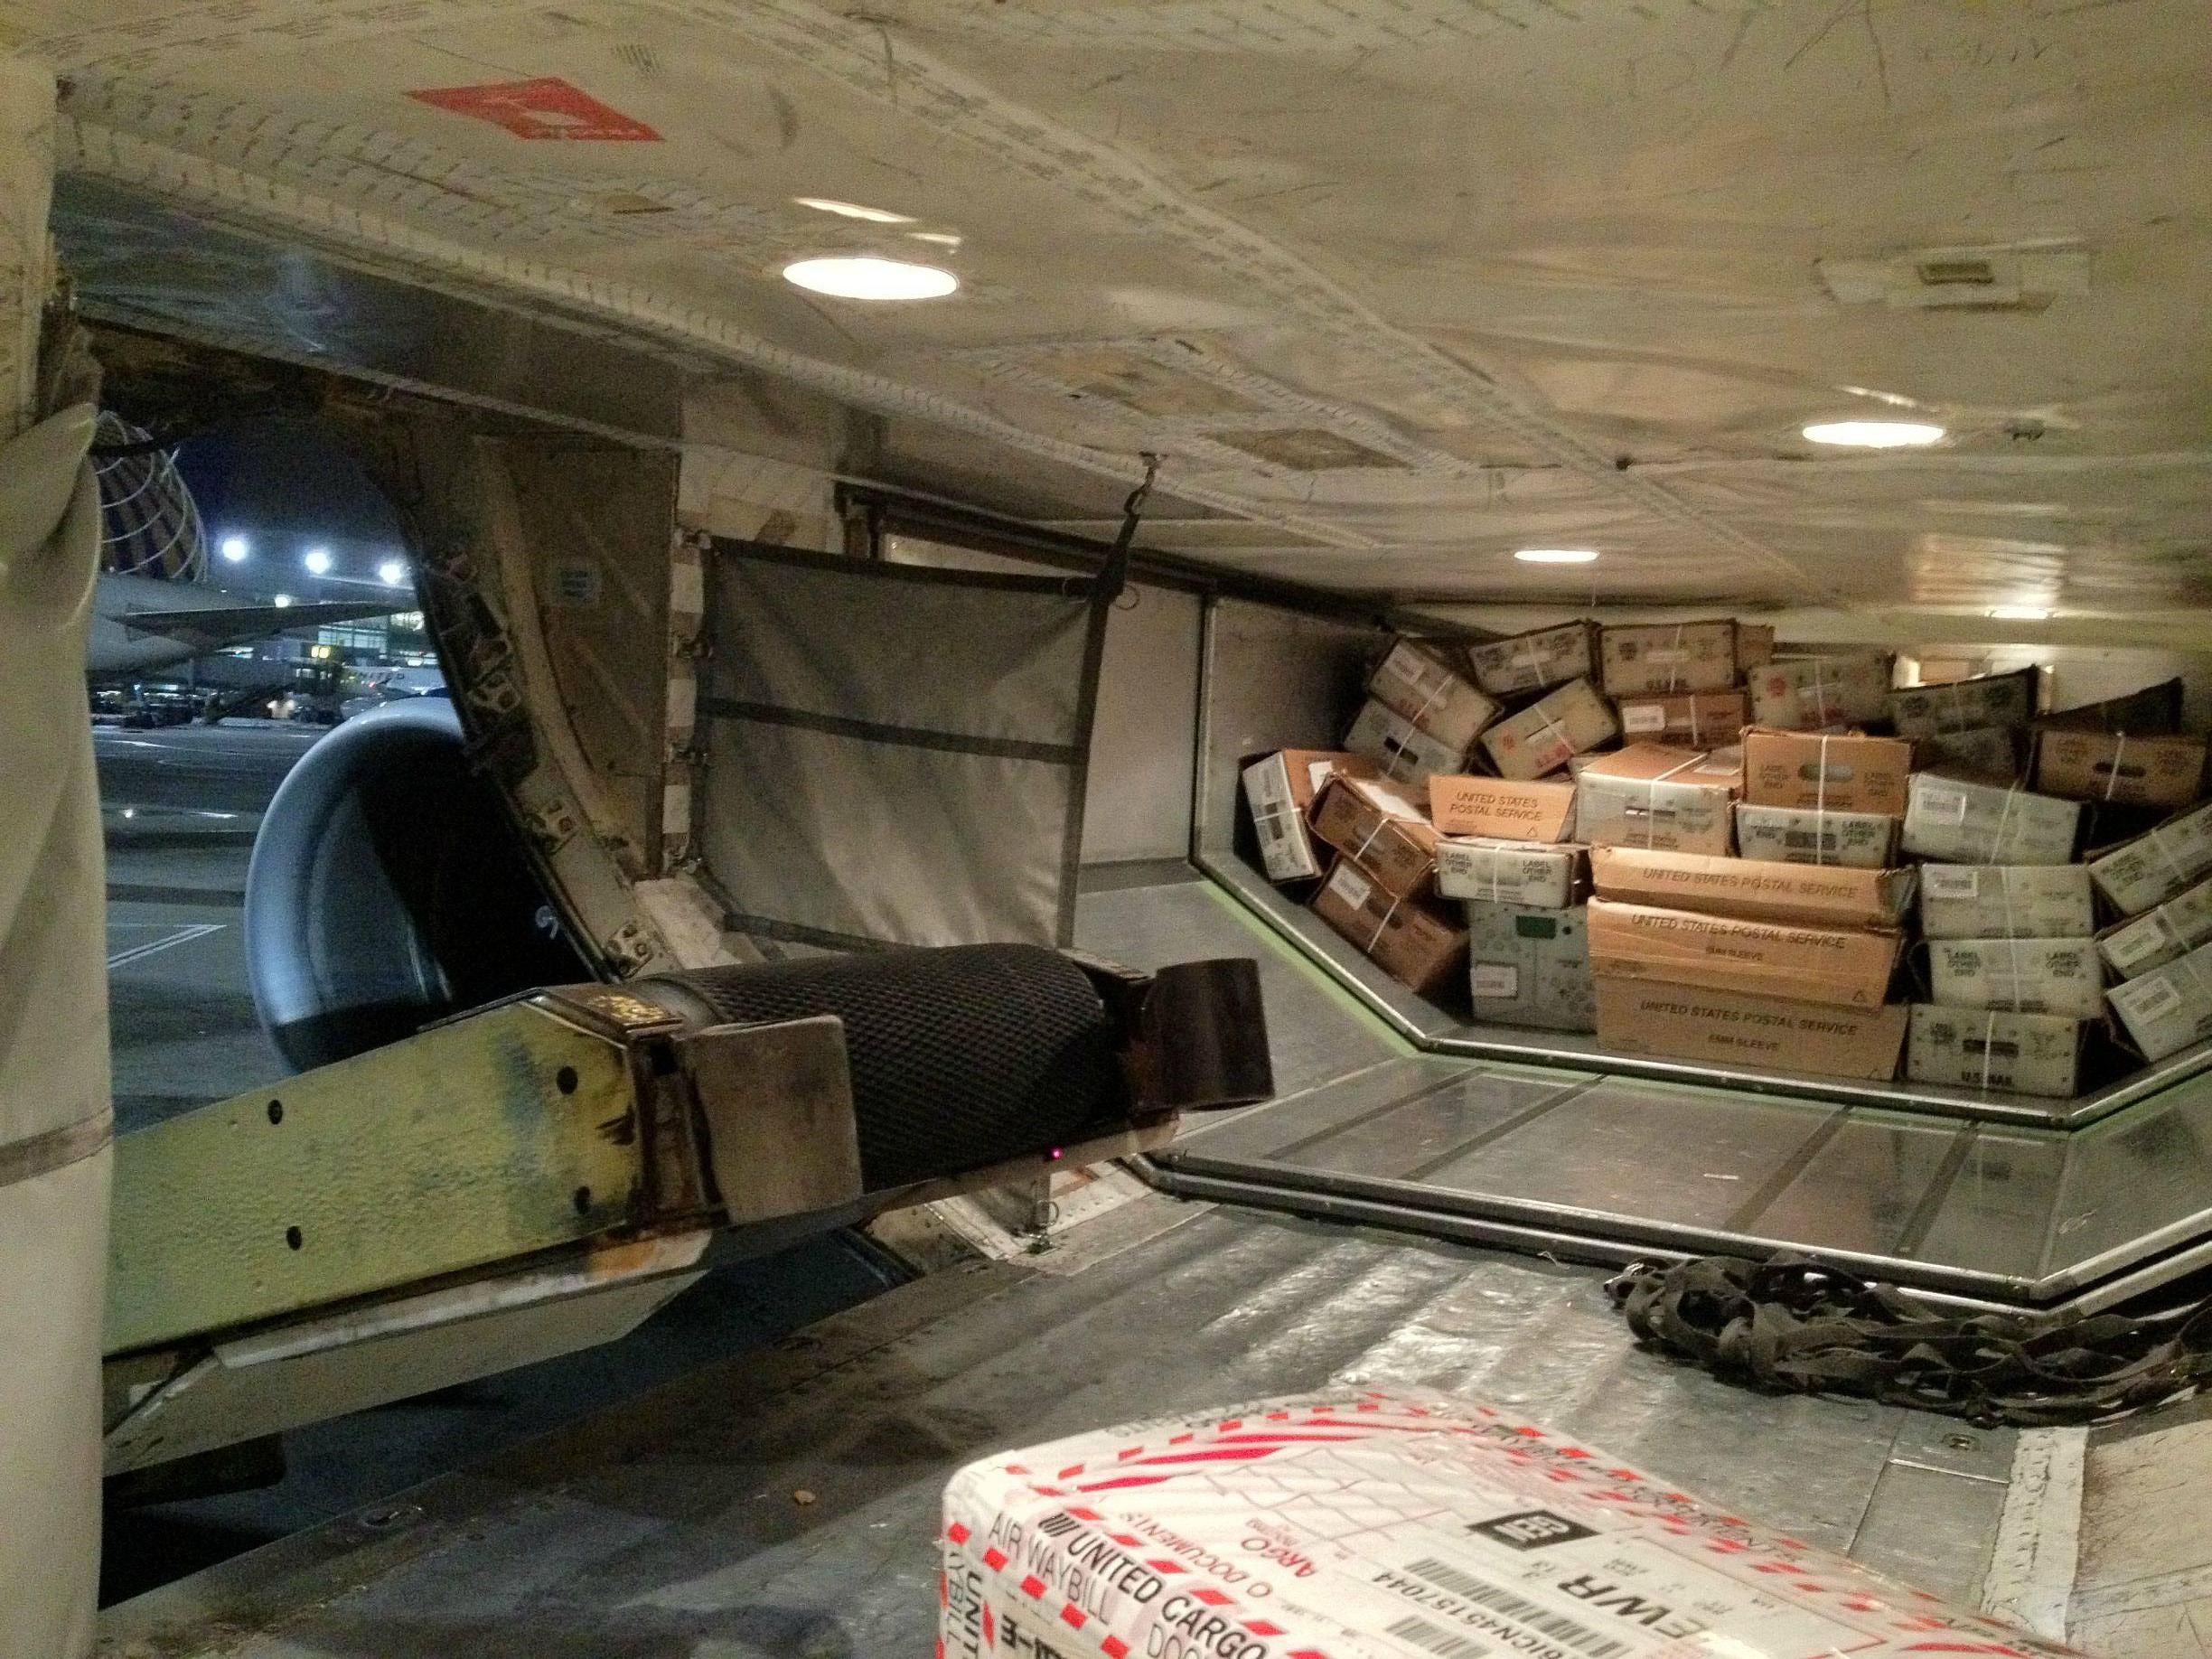
\includegraphics[width=0.7\textwidth]{CargoHoldClutter} \\
\textbf{Cargo hold clutter}
\end{figure}
\end{minipage}
\begin{minipage}[b]{0.45\linewidth}
\centering
\movie[width=0.9\textwidth,height=0.39\textwidth,poster,autostart,loop,borderwidth]{}{FireHotCenter.avi} \\
\movie[width=0.9\textwidth,height=0.39\textwidth,poster,autostart,loop,borderwidth]{}{FireHotRight.avi} \\
\textbf{Effect of Source Position}
\end{minipage}
\end{frame}
\begin{frame}
\frametitle{Motivation}
\label{sec-5-4}

\begin{itemize}
\item \textbf{Experiments are expensive}
\begin{itemize}
\item Destructive full-scale cargo hold fire experiments (FAA Tech Center)\footnote{Oztekin, E. S. Modeling of smoke spread and gas
transport in an aircraft. 7$^{th}$ International Fire and Cabin Safety
Research Conference, 2013.
 }
\item Each experiment destroys an entire cargo hold
\item Investigating boundary condition uncertainty is not feasible
\end{itemize}
\end{itemize}
\centering
\begin{minipage}[b]{0.45\linewidth}
\begin{figure}[ht]
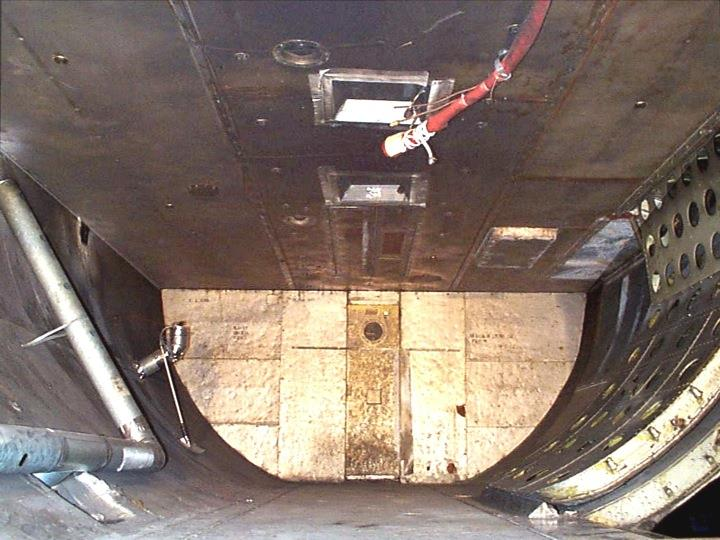
\includegraphics[width=0.9\textwidth]{Boeing707CargoHold} \\
\textbf{Boeing 707 cargo hold}
\end{figure}
\end{minipage}
\begin{minipage}[b]{0.45\linewidth}
\begin{figure}[ht]
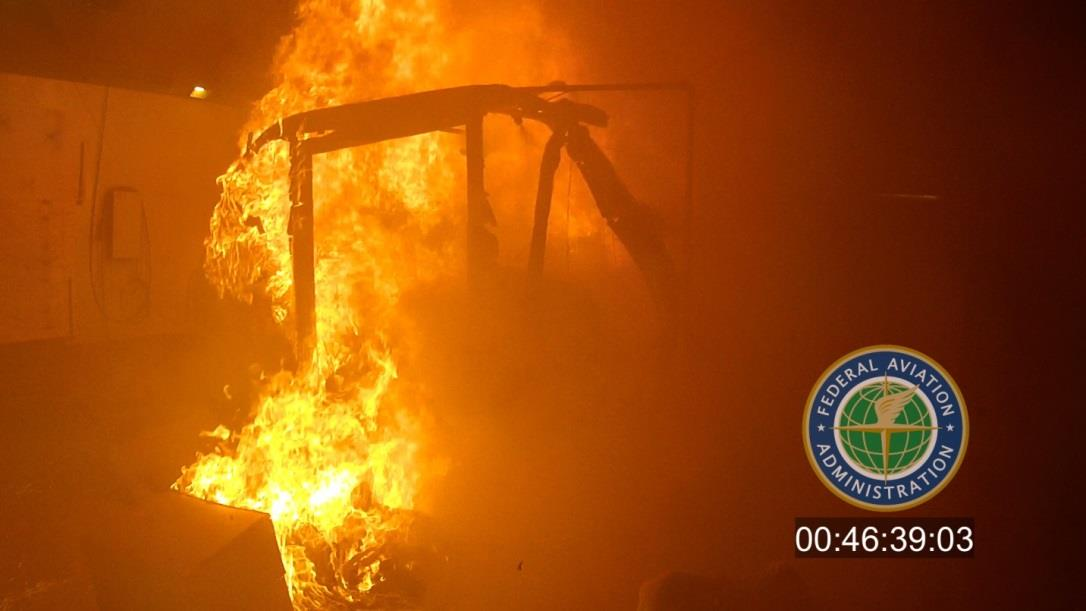
\includegraphics[width=0.9\textwidth]{CargoHoldFire1.png} \\
\textbf{Destructive cargo hold fire experiment}
\end{figure}
\end{minipage}
\end{frame}
\begin{frame}
\frametitle{Motivation}
\label{sec-5-5}

\begin{itemize}
\item \textbf{Computational methods must be accurate}
\begin{itemize}
\item Previous attempts at applying CFD to cargo hold fires have used
    low-order finite-volume solvers on meshes that do not conform to
    boundary\footnote{Oztekin, E.S et. al. Flow induced by a small fire in
an aircraft cargo compartment. AIAA 2012-0311.
 }
\end{itemize}
\end{itemize}
\centering
\begin{figure}[ht]
\includegraphics[width=0.7\textwidth]{CutCellGeometry.png} \\
\textbf{Non-conformal Cartesian mesh}
\end{figure}
\end{frame}
\begin{frame}
\frametitle{Motivation}
\label{sec-5-6}

\begin{itemize}
\item \textbf{Computational methods must be accurate}
\begin{itemize}
\item Vorticity dominated, buoyancy-driven flows require high
    computational accuracy
\end{itemize}
\end{itemize}
\centering
\movie[width=0.7\textwidth,height=0.525\textwidth,poster,autostart,loop,borderwidth]{}{N1_N2_N3.avi} \\
\textbf{Discontinuous Galerkin using varying degrees of accuracy}
\end{frame}
\begin{frame}
\frametitle{Objectives}
\label{sec-5-7}

\begin{itemize}
\item \textbf{Apply accurate CFD tools to the cargo hold problem}
\begin{itemize}
\item Boundary-fitted meshes for good boundary resolution
\item Discontinuous Galerkin (DG) high-order method for high accuracy
\end{itemize}
\item \textbf{Apply UQ tools to study effects of uncertainty in cargo hold problem}
\begin{itemize}
\item Polynomial Chaos Expansions (PCE)
\item Efficient sampling methodology
\item Accurate surrogate construction
\end{itemize}
\item Methodology gives (1) accurate computational tool for simulating
  cargo hold fires and (2) efficient framework for investigating cargo
  hold uncertainty
\end{itemize}
\end{frame}
\section{Fires: Methodology}
\label{sec-6}
\begin{frame}
\frametitle{Discontinuous Galerkin (DG) Method}
\label{sec-6-1}

\begin{itemize}
\item High-resolution CFD method\footnote{Wang et. al. An eulerian-lagrangian DG method for transient advection-diffusion equations. \emph{Numerical Methods for Partial Differential Equations}, 2007.
 }\textsuperscript{,}\,\footnote{Hesthaven \& Warburton. \emph{Nodal Discontinuous Galerkin Methods}, 2008.
 }
\begin{itemize}
\item Domain is divided into cells, collocation nodes computed within each cell
\item N-S equations projected onto span of polynomials (of arbitrary degree)
\item Flow variables within each cell represented in polynomial basis
\end{itemize}
\end{itemize}
\begin{figure}
\includegraphics[width=0.5\linewidth]{errorvscostzj.png} \\
\textbf{Generic error vs cost plot}
\end{figure}
\end{frame}
\begin{frame}
\frametitle{Discontinuous Galerkin (DG) Method}
\label{sec-6-2}

\textbf{Method Synopsis}
\beqq
\begin{aligned}
\text{Conservation law:}\quad & \diff{\bv{u}}{t} + \nabla \cdot \bv{f}(\bv{u}) = 0 \\
\text{Weak formulation:}\quad & \int_V \diff{\bv{u}}{t} \phi_j \ dV + \int_V  \nabla \cdot \bv{f}(\bv{u})\phi_j\ dV = 0 \\
\text{Integrate by parts:}\quad & \int_V \diff{\bv{u}}{t} \phi_j\ dV - \int_V \nabla \phi_j \cdot \bv{f}\ dV + \oint_S \phi_j \bv{\hat{f}} \cdot \bv{\hat{n}}\ dS = 0 \\
\ \bv{u}\approx \sum \bv{u}_i \phi_i\text{:}\quad & \int_V \diff{\bv{u}_i \phi_i}{t} \phi_j\ dV - \int_V \nabla \phi_j \cdot \bv{f}_i \phi_i\ dV + \oint_S \phi_j \bv{\hat{f}}_i \phi_i \cdot \bv{\hat{n}}\ dS = 0 \\
\text{}\quad & \bv{M}_{ij} \frac{d\bv{u}_i}{dt} = \int_V \nabla \phi_j \cdot \bv{f}_i \phi_i\ dV + \oint_S \phi_j \bv{\hat{f}}_i \phi_i \cdot \bv{\hat{n}}\ dS \\
\end{aligned}
\eeqq
\textbf{Polynomial Basis}
\begin{itemize}
\item Collocation nodes are defined in each individual cell
\item Chebyschev-like schemes used (to avoid Runge-phenomenon)
\item Associated Lagrange interpolators form the polynomial basis ${\phi_k}$
\end{itemize}
\end{frame}
\begin{frame}
\frametitle{Discontinuous Galerkin (DG) Method}
\label{sec-6-3}

\textbf{Time-Stepping}
\begin{itemize}
\item We now have a system of ODEs to solve for each DG mode:
\end{itemize}
$$\frac{d\bv{u}}{dt} = \bf{f}(\bf{u,u',t})$$
\begin{itemize}
\item CFL condition for explicit time-stepping gives $\Delta t = O(\frac{\Delta x}{N^2})$
\begin{itemize}
\item Mesh volume $\Delta x$ can be small
\item State dimension $N$ grows rapidly with increasing polynomial order
\end{itemize}
\item Thus, implicit time-stepping is used, which gives the large nonlinear system:
  $$\bv{F}(\bv{u}) = 0$$
\end{itemize}
\end{frame}
\begin{frame}
\frametitle{Discontinuous Galerkin (DG) Method}
\label{sec-6-4}

\textbf{Solution Procedure}
\begin{itemize}
\item Newton's method gives sequence of linear systems:
\end{itemize}
$$\bv{J}(\bv{u^{k}}) \delta \bv{u^k} = -\bv{F}(\bv{u^{k}}),\quad \bv{u^{k+1}}=\bv{u^{k}}+\delta \bv{u^k}$$
\begin{itemize}
\item $\bv{J}$ is prohibitively large to compute/store
\item Jacobian-Free Newton-Krylov iteration
\begin{itemize}
\item Action of Jacobian on a vector is approximated as:
\end{itemize}
$$ \bv{J} \bv{v} \approx [\bv{F}(\bv{u} + \epsilon \bv{v}) - \bv{F}(\bv{v})]/\epsilon$$
\begin{itemize}
\item $\delta \bv{u}^k$ is solved for using Krylov iteration (GMRES, BiCGSTAB)
\end{itemize}
\end{itemize}
\end{frame}
\begin{frame}
\frametitle{Polynomial Chaos Expansions (PCE)}
\label{sec-6-5}

\begin{itemize}
\item Overview\footnote{Xiu \& Karniadakis. The weiner-askey polynomial chaos for stochastic differential equations. \emph{SIAM Journal of Scientific Computing}, 2002.
 }:
\begin{itemize}
\item Method for quantifying parametric uncertainty
\item Expand output in terms of basis polynomial functions of random variables
\end{itemize}
$$f(\xi) &\approx \sum_{i}^N a_i \psi_i(\xi)$$
\item Pros:
\begin{itemize}
\item Efficient sampling methodology
\item Explicit surrogate model
\item Easy statistical post-processing (eg., sampling, ANOVA)
\end{itemize}
\end{itemize}
\fontsize{9}\selectfont
% Define the layers to draw the diagram
\pgfdeclarelayer{background}
\pgfdeclarelayer{foreground}
\pgfsetlayers{background,main,foreground}

% Define block styles used later

\tikzstyle{sensor}=[draw, fill=blue!20, text width=5em, 
    text centered, minimum height=2.5em,drop shadow]
\tikzstyle{ann} = [above, text width=5em, text centered]
\tikzstyle{wa} = [sensor, text width=10em, fill=blue!20, 
    minimum height=7em, rounded corners, drop shadow]

% Define distances for bordering
\def\blockdist{2.3}
\def\edgedist{2.5}

\begin{tikzpicture}
    \node (CleanAirfoil) [wa]  {\includegraphics[width=0.9\textwidth]{ExamplePDF}\\\textbf{Input}};
    \path (CleanAirfoil)+(4,0) node (FlowSolver) [wa] {\textbf{Computation/}\\\textbf{Experiment}};
    \path (FlowSolver)+(4,0) node (Droplet) [wa] {\includegraphics[width=0.9\textwidth]{ExamplePDF2}\\\textbf{Output}};

    \path [draw, ->, thick] (CleanAirfoil.east) |- node [right] {} (FlowSolver.west);
    \path [draw, ->, thick] (FlowSolver.east) -- node [right] {} (Droplet.west);
            
\end{tikzpicture}
\end{frame}
\begin{frame}
\frametitle{Polynomial Chaos Expansions (PCE)}
\label{sec-6-6}

\textbf{Setting}
\begin{itemize}
\item Stochastic input process parameterized by $d$ independent random
  variables $\xi_1 \cdots \xi_d$ with joint PDF $\rho(\xi)$
\item Objective: approximate statistical dependence of an output variable $f(\xi)$
\end{itemize}
\textbf{Method Synopsis}
\beqq
\begin{aligned}
\text{Polynomial basis:} \quad & \lbrace \psi_k \rbrace_{k=1}^{\infty} \quad , \quad \langle \psi_i , \psi_j \rangle = \delta_{ij} \\
&\langle f , g \rangle = \int_{\Gamma} f(\xi) g(\xi) \rho(\xi) d\xi \\
\text{Output Representation:} \quad & f(\xi) \approx \sum_{i}^N a_i \psi_i(\xi) \\
\text{Projection:} \quad & a_k = \frac{\langle f,\psi_k \rangle}{\| \psi_k \|^2} \\
\text{Quadrature:} \quad & \langle f,\psi_k \rangle \approx \sum_{i=1}^Q f(\xi^i) \psi_k(\xi^i) w^i \\
\end{aligned}
\eeqq
\end{frame}
\begin{frame}
\frametitle{Polynomial Chaos Expansions (PCE)}
\label{sec-6-7}

\begin{figure}[ht]
\centering
\begin{minipage}[b]{0.45\linewidth}
\includegraphics[width=0.7\textwidth]{MonteCarlo} \\
\centering
\textbf{Monte Carlo} \\
\begin{equation*}
  y \approx \delta(\xi - \xi_k)
\end{equation} \\
\begin{itemize}
\item Draw random samples
\item Data exist at discrete points
\end{itemize}
\end{minipage}
\begin{minipage}[b]{0.45\linewidth}
\includegraphics[width=0.7\textwidth]{QuadraturePoints} \\
\centering
\textbf{Polynomial Chaos}
\begin{equation*}
  y \approx \sum_{i}^{Q} c_i \psi_i(\xi)
\end{equation} \\
\begin{itemize}
\item Take data at collocation points
\item Construct global surrogate
\end{itemize}
\end{minipage}
\end{figure}
\end{frame}
\section{Fires: Example study}
\label{sec-7}
\begin{frame}
\frametitle{Input Processes}
\label{sec-7-1}

\textbf{Parameters: Fire source temperature and location}
\begin{itemize}
\item Empty cargo hold
\item Uniform distribution for both independent parameters
\end{itemize}
\fontsize{9}\selectfont
% Define the layers to draw the diagram
\pgfdeclarelayer{background}
\pgfdeclarelayer{foreground}
\pgfsetlayers{background,main,foreground}

% Define block styles used later

\tikzstyle{basic}=[draw, fill=blue!20, text width=5em, 
    text centered, minimum height=2.5em,drop shadow]
\tikzstyle{mode} = [basic, text width=10em, fill=blue!20, 
    minimum height=4em, rounded corners, drop shadow]

% Define distances for bordering
\def\blockdist{2.3}
\def\edgedist{2.5}
\centering
\begin{tikzpicture}
    \node (ColdLeft) [mode]  {\includegraphics[width=0.9\textwidth]{ColdLeft}};
    \path (ColdLeft)+(6,0) node (HotLeft) [mode] {\includegraphics[width=0.9\textwidth]{HotLeft}};
    \path (ColdLeft)+(0,-3) node (ColdRight) [mode] {\includegraphics[width=0.9\textwidth]{ColdRight}};
    \path (ColdRight)+(6,0) node (HotRight) [mode] {\includegraphics[width=0.9\textwidth]{HotRight}};

    \path [draw, ->, thick] (ColdLeft.east) |- node [right=1.3cm,above=2mm] {Temperature} (HotLeft.west);
    \path [draw, ->, thick] (ColdLeft.south) -- node [left=0.25cm,down] {Position} (ColdRight.north);
    \path [draw, ->, thick] (ColdLeft.south east) -- node [left] {} (HotRight.north west);

    \begin{pgfonlayer}{background}
        \path (ColdLeft.west)+(-1,1) node (a) {};
        \path (HotRight.east)+(1,-1) node (b) {};
        \path[fill=orange!20,rounded corners, draw=black!50, dashed] (a) rectangle (b);
    \end{pgfonlayer}
\end{tikzpicture}
\end{frame}
\begin{frame}
\frametitle{Input Processes}
\label{sec-7-2}

\textbf{Parameters: Fire source temperature and location}
\begin{itemize}
\item Empty cargo hold
\item Uniform distribution for both independent parameters
\end{itemize}
\fontsize{9}\selectfont
% Define the layers to draw the diagram
\pgfdeclarelayer{background}
\pgfdeclarelayer{foreground}
\pgfsetlayers{background,main,foreground}

% Define block styles used later

\tikzstyle{basic}=[draw, fill=blue!20, text width=5em, 
    text centered, minimum height=2.5em,drop shadow]
\tikzstyle{mode} = [basic, text width=10em, fill=blue!20, 
    minimum height=4em, rounded corners, drop shadow]

% Define distances for bordering
\def\blockdist{2.3}
\def\edgedist{2.5}
\centering
\begin{tikzpicture}
    \node (ColdLeft) [mode]  {\movie[width=0.9\textwidth,height=0.39\textwidth,poster,autostart,loop,borderwidth]{}{FireColdCenter.avi}};
    \path (ColdLeft)+(6,0) node (HotLeft) [mode] {\movie[width=0.9\textwidth,height=0.39\textwidth,poster,autostart,loop,borderwidth]{}{FireHotCenter.avi}};
    \path (ColdLeft)+(0,-3) node (ColdRight) [mode] {\movie[width=0.9\textwidth,height=0.39\textwidth,poster,autostart,loop,borderwidth]{}{FireColdRight.avi}};
    \path (ColdRight)+(6,0) node (HotRight) [mode] {\movie[width=0.9\textwidth,height=0.39\textwidth,poster,autostart,loop,borderwidth]{}{FireHotRight.avi}};

    \path [draw, ->, thick] (ColdLeft.east) |- node [right=1.3cm,above=2mm] {Temperature} (HotLeft.west);
    \path [draw, ->, thick] (ColdLeft.south) -- node [left=0.25cm,down] {Position} (ColdRight.north);
    \path [draw, ->, thick] (ColdLeft.south east) -- node [left] {} (HotRight.north west);

    \begin{pgfonlayer}{background}
        \path (ColdLeft.west)+(-1,1) node (a) {};
        \path (HotRight.east)+(1,-1) node (b) {};
        \path[fill=orange!20,rounded corners, draw=black!50, dashed] (a) rectangle (b);
    \end{pgfonlayer}
\end{tikzpicture}
\end{frame}
\begin{frame}
\frametitle{Output Measurements}
\label{sec-7-3}

\textbf{Problem}
\begin{itemize}
\item UQ for the entire flow field is difficult
\begin{itemize}
\item Spatio-temporal behavior varies significantly
\item Need a more tractable set of observables
\end{itemize}
\end{itemize}
\textbf{Solution}
\begin{itemize}
\item Reduce spatial dimensionality
\begin{itemize}
\item Ceiling temperature is most important for detection
\end{itemize}
\item Separate time and space
\begin{itemize}
\item \emph{Intuition}: buoyant plumes convect upwards at some characteristic
    time $t_R$ dominated by source temperature
\item Easier to compare ceiling temperatures at their respective values
    of $t_R$ than at same time after ignition
\end{itemize}
\end{itemize}
\textbf{Output Measurements}
\begin{equation*}
\begin{aligned}
t_R(Z) &= \text{(Rise time)} \\
\overbar{T_C}(x;Z) &= \frac{1}{\Delta t} \int_{t_R(Z)}^{t_R(Z)+\Delta t} T_C(x,t;Z) dt
\end{aligned}
\end{equation}
\end{frame}
\begin{frame}
\frametitle{Results: Rise Time}
\label{sec-7-4}


\centering
\begin{minipage}[b]{0.45\linewidth}
\begin{figure}[ht]
\includegraphics[width=0.9\textwidth,trim = 40mm 0mm 40mm 0mm,clip]{PCEMapTR_matplotlib} \\
\textbf{PCE surrogate map of $t_R(Z)$} \\
\end{figure}
\begin{itemize}
\item $t_R$ is dominated by source temperature
\item Clearly, hotter source gives shorter rise time
\end{itemize}
\end{minipage}
\begin{minipage}[b]{0.45\linewidth}
\begin{figure}[ht]
\includegraphics[width=0.9\textwidth]{PCEStatTR_matplotlib} \\
\textbf{Probability density function} \\
\end{figure}
\begin{itemize}
\item Nonlinear mapping deforms (initially uniform) PDF
\item Tail caused by low temperature and wall effect
\end{itemize}
\end{minipage}
\end{frame}
\begin{frame}
\frametitle{Results: Ceiling Temperature}
\label{sec-7-5}


\centering
\begin{minipage}[b]{0.45\linewidth}
\begin{figure}[ht]
\includegraphics[width=0.9\textwidth]{CeilingTempMeanPercentiles} \\
\textbf{Mean and Confidence Intervals}
\end{figure}
\end{minipage}
\begin{minipage}[b]{0.45\linewidth}
\begin{figure}[ht]
\includegraphics[width=0.9\textwidth]{SobolIndexCeilingTemp} \\
\textbf{Sobol indices}
\end{figure}
\end{minipage}

\begin{minipage}[t]{0.45\linewidth}
\begin{itemize}
\item ({\color{blue} 68$\%$}, {\color{red} 95$\%$}) C.I.
\item Profile skewed right of center
\item Wide variation in temperature range and locations possible
\end{itemize}
\end{minipage}
\begin{minipage}[t]{0.45\linewidth}
\begin{itemize}
\item ({\color{blue} $x_S$}, {\color{red} $T_S$})
\item Fraction of variance attributable to each individual parameter
\item {\color{red} $T_S$}: dominant near maximum
\item {\color{blue} $x_S$}: dominant near periphery
\end{itemize}
\end{minipage}
\end{frame}
\begin{frame}
\frametitle{Results: Related Statistics}
\label{sec-7-6}


\centering
\begin{minipage}[b]{0.45\linewidth}
\begin{figure}[ht]
\includegraphics[width=0.9\textwidth]{maxCeilingTempDistribution} \\
\textbf{PDF of max($T_C$)}
\end{figure}
\end{minipage}
\begin{minipage}[b]{0.45\linewidth}
\begin{figure}[ht]
\includegraphics[width=0.9\textwidth]{maxCeilingTempLocationDistribution} \\
\textbf{PDF of Location(max($T_C$))}
\end{figure}
\end{minipage}

\begin{itemize}
\item Can estimate statistics of quantities derived from output measurements
\item The maximum ceiling temperature and its location are of practical engineering interest
\item For this example, a temperature sensor must:
\begin{itemize}
\item Be able to detect temperatures roughly in the range $T_C \in [1.05,1.35] \times T_{\infty}$
\item Be placed on the ceiling in roughly in the range $x_C \in [-0.25, 0.5]$
\end{itemize}
\end{itemize}
\end{frame}
\begin{frame}
\frametitle{Conclusions/Future Work}
\label{sec-7-7}


\textbf{Problem}
\begin{itemize}
\item Airfoil icing/cargo hold fire safety is important and subject to uncertainty
\item Experiments are expensive
\item CFD methods must be high-resolution
\end{itemize}
\textbf{Solutions: Icing}
\begin{itemize}
\item Data-based modeling of shape variation
\item Computational-based UQ
\end{itemize}
\textbf{Solutions: Fires}
\begin{itemize}
\item Discontinuous-Galerkin solver for high CFD resolution
\item Polynomial Chaos for efficient sampling and accurate surrogate/statistics
\end{itemize}
\textbf{Future Work: Fires}
\begin{itemize}
\item Cargo holds in practice are not empty
\item Extend framework to handle cargo hold clutter (baggage, pipes, etc.)
\end{itemize}
\textbf{Future Work: Icing}
\begin{itemize}
\item Extend efforts to 3D wing icing
\item Continue development and testing of icing code
\item Use icing code to investigate statistical variation of ice shape
\end{itemize}
\end{frame}

\end{document}
